\documentclass[mphil, 12 pt]{csthesis}


% \usepackage{CJKutf8}

\usepackage{comment}

%% \usepackage[style=alphabetic]{biblatex}
\usepackage[square]{natbib}
%% \PassOptionsToPackage{authoryear}{natbib}
\usepackage{caption}
\usepackage{graphicx}
%\usepackage{subfigure}
\usepackage{changepage}
\usepackage{url}
\usepackage{subfig}

\usepackage{paralist}
\usepackage[pdfpagelabels]{hyperref}
\usepackage[all]{hypcap}
\usepackage{verbatim}
\usepackage{array}
\usepackage{float}
\usepackage{multirow}
\usepackage{rotating}
\usepackage{multicol}
\usepackage{longtable}
\usepackage{amsmath}

\usepackage{listings} 	
% "define" Scala
\lstdefinelanguage{scala}{
  morekeywords={abstract,case,catch,class,def,%
    do,else,extends,false,final,finally,%
    for,if,implicit,import,match,mixin,%
    new,null,object,override,package,%
    private,protected,requires,return,sealed,%
    super,this,throw,trait,true,try,%
    type,val,var,while,with,yield},
  otherkeywords={=>,<-,<\%,<:,>:,\#,@, <:<},
  sensitive=true,
  morecomment=[l]{//},
  morecomment=[n]{/*}{*/},
  morestring=[b]",
  morestring=[b]',
  morestring=[b]"""
}

\usepackage{pxfonts}
\usepackage{color}
\definecolor{dkgreen}{rgb}{0,0.6,0}
\definecolor{gray}{rgb}{0.5,0.5,0.5}
\definecolor{mauve}{rgb}{0.58,0,0.82}
\definecolor{blue}{rgb}{0,0,1}
 
% Default settings for code listings
\lstset{frame=tb,
  language=scala,
  aboveskip=3mm,
  belowskip=3mm,
  showstringspaces=false,
  columns=flexible,
  basicstyle={\small\ttfamily},
  numbers=left, % none,
  numbersep=2pt,
  numberstyle=\tiny\color{gray},
  keywordstyle=\bfseries\color{black},
  commentstyle=\color{dkgreen},
  stringstyle=\color{mauve},
  frame=none, % single,
  breaklines=true,
  breakatwhitespace=true,
  tabsize=2,
  captionpos=b
}

% A comment in a draft (shouldn't appear in the final version).
\newcommand{\mycomment}[1]{\(\spadesuit\){\bf #1 }\(\spadesuit\)}
% Comment this out in the draft
% \newcommand{\mycomment}[1]{}
\newcommand{\pmcomment}[1]{\comment{PM}{#1}}
\newcommand{\pwtcomment}[1]{\comment{PT}{#1}}
\newcommand{\rscomment}[1]{\comment{RS}{#1}}

% line break in table.  e.g.
% Foo bar & \specialcell{Foo\\bar} & Foo bar \\    % vertically centered
% Foo bar & \specialcell[t]{Foo\\bar} & Foo bar \\ % aligned with top rule
\newcommand{\specialcell}[2][c]{%
  \begin{tabular}[#1]{@{}c@{}}#2\end{tabular}}

%% reset footnote counter each page
\makeatletter
\@newctr{footnote}[page]
\makeatother

\begin{document}

% \markboth{V. F. Pamplona et al.}{Photorealistic Models for Pupil Light Reflex and Iridal Pattern Deformation}

\title{Type-parameterized Actors and Their Supervision}
\author{Jiansen HE}
\submityear{2014}

\maketitle 

%\dedication{


\section*{Acknowledgements}

This thesis is dedicated to my parents for their endless love and support.
It is also dedicated to my wife, Shiye, for her continuous encouragement
during my hard times.  Meeting my wife and getting married are the best
two things happened to me in the past 4 years.

I want to thank my supervisors, Philip Wadler, Philip Trinder and Don Sannella,
for their guidance over four years.  I am fortunate to have been supervised
by them.

I gratefully acknowledge the substantial help that have received from many 
colleagues who have shared their related results and ideas over the long period 
during which this thesis was in preparation. Benedict Kavanagh and Danel Ahman 
for continuous comments and discussions. Roland Kuhn from the Akka team for 
sharing deep insight of the the Akka design.  
The RELEASE team for giving us access to the source code of the BenchErl 
benchmark examples.  Thomas Arts from QuviQ.com and Francesco Cesarini from 
Erlang Solutions for providing the Erlang source code of two examples used 
in their commercial training courses.



%}

\setcounter{tocdepth}{1}
\standarddeclaration
\oneandahalfspace
\tableofcontents

% \begin{comment}

\begin{abstract}

The robustness of actor-based concurrent applications can be improved upon by 
(i) employing failure recovery mechanisms such as the supervision principle, or 
(ii) using typed messages to prevent ill-typed communication. This thesis 
introduces TAkka, a typed Akka library that supports both the supervision 
principle and typed messages. The TAkka library mixes static and dynamic type 
checking to make sure that dynamically typed distributed resources and 
statically typed local resources have consistent types. Our notion of typed 
actor can publish itself as different types when used by different parties so 
that messages of unexpected types are prevented at the senders' side. In TAkka, 
messages for supervision purposes are treated in a special way so that a 
supervisor can interact with child actors of different types. Results show that 
Akka programs can be gradually upgraded to TAkka equivalents with minimal 
runtime and code size overheads. Finally, TAkka includes two auxiliary 
libraries for reliability assessment.

\end{abstract}

% \end{comment}

 \chapter{Introduction}

This introductory chapter presents the general background that motivates solving  problems discussed in this thesis.  It summarizes main contributions of this thesis.  Finally, an overview of the thesis is given.

\section{General Background and Motivation}

Building reliable distributed applications is among the most difficult tasks 
facing programmers, and one which is becoming increasingly important due to the 
recent advent of web applications, cloud services, and mobile apps.  Modern 
society relies on distributed applications which are executed on heterogeneous 
runtime environments, are tolerant of partial failures, and sometimes 
dynamically upgrade some of their components without affecting other parts.

A distributed application typically consists of components which handle some 
tasks independently, while collaborating on other tasks by exchanging
messages.  The robustness of a distributed application, therefore, 
can be improved by (i) using a fault-tolerant design to minimise the 
aftermath of partial failures, or (ii) employing type checking to detect 
some errors, including the logic of component implementations, and 
communications between components.

One of the most influential fault-tolerant designs is the supervision 
principle, proposed in the first release of the Erlang/OTP library in 1997 
\citep{OTP}. The supervision principle states that concurrent components of an 
application should be encapsulated as actors, which make local decisions in 
response to received messages.  Actors form a tree structure, where a parent 
node is responsible for monitoring its children and restarting them when 
necessary. The supervision principle is proposed to increase the robustness of 
applications written in Erlang, a dynamically typed programming language.  
Erlang application developers can employ the supervision principle by using 
related API from the Erlang/OTP library.  It is reported that the supervision 
principle helped AXD301, an ATM (Asynchronous Transfer Mode) switch 
manufactured by Ericsson Telecom AB. for British Telecom, to achieve 
99.9999999\% (9 nines) uptime during a nine-month test \citep{ArmstrongAXD}. 
Nevertheless, adopting the Supervision principle is optional in Erlang 
applications.

Aside from employing good design patterns, programmers can use typed 
programming languages to construct reliable and maintainable 
programs.  Typed programming languages have the advantages of detecting some 
errors earlier, enforcing disciplined and modular programming, providing 
guarantees on language safety, and efficiency optimisation \citep{TPL}.

Can programmers benefit from the advantages of both the 
supervision tree and type checking?  In fact, attempts have been made in two 
directions: statically type checking Erlang programs and porting the 
supervision principle to statically typed systems.

Static checking in Erlang can be done via optional checking tools or 
rewriting applications using an Erlang variant that uses a statically typed 
system.  Static analysis tools of Erlang include the Dialyzer \citep{Dialyzer} 
and a fault tolerance analysis tool by \citet{JanHenry}.  The Dialyzer tool is 
shipped with Erlang.  It has identified a number of unnoticed errors in large 
Erlang applications that have been run for many years 
\citep{DialyzerDetecting}. Nevertheless, the use of Dialyzer and other 
analysis tools is often involved in the later stages of Erlang applications 
development.  In comparison with static analysis tools, simplified Erlang 
variants that use static type systems have been designed by 
\citet{marlow1997practical}, \citet{sabelfeld2002securing}, among others.  As 
the expressiveness is often sacrificed in those simplified variants to some 
extent, code modifications are more or less required to make existing 
Erlang programs go through the type checker.

The second attempt is porting the notion of actors and supervision trees to 
statically typed languages, including Scala and Haskell.  Scala actor 
libraries, 
including Scala Actors \citep{actor_1, actor_2} and Akka 
\citep{akka_api,akka_doc}, use 
dynamically typed messages even though Scala is a statically typed language.  
Some recent actor libraries, including Cloud Haskell \citep{CloudHaskell}, Lift 
\citep{lift_scala}, and scalaz \citep{scalaz}, support both 
dynamically and statically typed messages, but do not support supervision.  Can 
actors in supervision trees be statically typed? 

The key claim in this thesis is that actors in supervision trees can be 
statically typed by parameterizing the actor class with the type of messages it 
expects to receive.  This research project is motivated by the following benefits of statical typing:
\begin{enumerate}
  \item Both users and developers of actor-based services can take advantages 
of type-parameterized actors.  For users, sending ill-typed messages is 
prevented at compile time.  Because messages are usually transmitted 
asynchronously, it may be otherwise difficult to trace the source of errors at 
runtime, especially in distributed environments.  For service developers, since 
unexpected messages are eliminated from the system, they can focus on the 
logic of the services rather than worrying about incoming messages of 
unexpected types.  Another immediate benefits of typing checking is pattern
completeness checking for message handlers.
  \item Static typing enforces disciplined and modular programming \citep{TPL}.
Opposite to writing programs in dynamically typed languages, programers are often more confident to use complex and deep nested types in statically typed languages.  Using complex types that have a higher level of abstraction improves the readability and maintainability of programs.  On the other side, porting nested types into an untyped system using nested tuples is possible but often results in complex code that is more difficult to understand.
  \item Static typing often results in shorter code \citep{TPL}.  When a new actor is defined, handlers for ill-typed messages are no longer needed.  When an application is built on top of some actors, which are often black boxes to application developers, there is no need to study how those actors will behave upon receiving unexpected messages and implement handlers for every problematic cases.
  \item A statically typed program can often be compiled to code that executes more quickly \citep{TPL}.  As the compiler knows the exact data types that are in use at runtime, ad hoc optimizations might be applied to the assembly code or the machine code.
  \item Statically typed interface is a clear and precise documentation per se \citep{TPL}.  Users of a type-parameterized actor understands its functionality immediately by looking at its type parameter, which denotes the type of permitted messages.  Without the type information, users would be more rely on good documentation, examples, and even small experiments created by themselves\citep{endrikat2014api}.

\end{enumerate}


Implementing type-parameterized actors in a statically-typed language, however, 
requires solving the following three problems:

\begin{enumerate}
  \item A typed name server is required to retrieve actor references of
specific types.  A distributed system usually requires a name server which
maps names of services to processes that implement that service.  If processes
are dynamically typed, the name server is usually implemented as a map from 
names to processes. Can a distributed name server maintain maps from the typed 
names and processes of corresponding types, and provide API for 
registering and fetching statically typed processes?

  \item A supervisor actor must interact with child actors of different types. 
Each actor in a supervision tree needs to handle messages for both the purpose 
of supervision and its own specific interests.  When all actors are 
parameterized by different types, is it practical to define a supervisor that 
communicates with children of different types?

  \item Actors that receive messages from distinct parties may suffer from the 
type pollution problem, whereby a party imports too much type information 
about an actor and can send the actor messages not expected from it. Systems 
built on a layered architecture or the MVC model are often victims of the type 
pollution problem. As an actor receives messages from distinct parties using its 
sole channel, its type parameter is the union type of all expected message 
types. Therefore, unexpected messages can be sent to an actor which naively 
publishes its type parameter or permits dynamically typed messages. Can a 
type-parameterized actor publish itself as different types when it communicates 
with different parties?
\end{enumerate}

\section{Contributions}

The overall goal of the thesis is to develop a framework that makes it possible 
to construct reliable distributed applications written using and validated by 
our library, TAkka, which merges the advantages of type checking and the 
supervision principle.   

The TAkka library is implemented in the Scala programming language.  It
expands the existing Akka library for supervised actors by the introduction 
of typed messaging.  Akka is developed at TypeSafe Inc.  
As Akka becomes part of the standard library in Scala 2.10 
and higher versions, it is widely used in many real applications.  Choosing 
Akka as the base of our design and implementation benefits this project in 
many aspects.  Firstly, the author checks that main requirements in distributed 
programming are not unintentionally neglected by rewriting 23 Akka applications 
written by other professional programmers.  Secondly, improvements made in 
the TAkka library can benefit existing Akka applications with a low cost because, 
as presented later, rewriting Akka applications using TAkka involves less than 10\% 
straightforward code changes.  Finally, despite some deficits in the Akka design, 
it saves the author a significant amount of work on low-level implementation.  
In fact, some less carefully designed Akka features have inspired the author to 
make improvements in the TAkka library.

Source code of the TAkka library, testing and demonstration examples, along with
other related documentations produced during this research are available at a 
GitHub repository for this project \citep{takka_repo} and the CD attached to this thesis.
A condensed version of the material in this thesis is published in a companion paper \citep{TAKKA_paper}.

Generally speaking, the key contributions of this thesis are:

\begin{itemize}
\begin{comment}
  \item A formal model that captures the essence of the supervision principle.  
  The model (Chapter~\ref{supervision_model}) exhibits key features of the 
  supervision principle used in existing libraries including Erlang, Akka, and 
  TAkka. It provides a tool to compare the design alternatives to the 
  supervision principle.  
\end{comment}  
  \item The design and implementation of the TAkka library (Chapter~\ref{takka_design}), where supervised 
actors are parameterized by the type of messages they expect.  The library 
  mixes static and dynamic type checking so that type
  errors are detected at the earliest opportunity.  The library separates 
  message types and message handlers for the purpose of supervision from those 
  for actor specific communications.  The decision is made so that   
  type-parameterized actors of different types can form a supervision tree. 
%  Interestingly, this decision coincides with our recommendation in the model 
%  analysis for improving availability.  
  Chapter~\ref{evolution} shows that Akka 
  programs can be upgraded to their TAkka equivalents incrementally, one module 
  at a time (evolution), rather 
  than requiring a monolithic change to all modules simultaneously (revolution).  The
  design is analogous to a design principle of Java Generics, known as ``Evolution,
  not Revolution''

  
  \item A framework for evaluating libraries that supports the supervision 
  principle. Chapter~\ref{takka_evaluation} shows that the type pollution 
  problem can be straightforwardly avoided in TAkka.  The evaluation further 
  compares the TAkka library and the Akka library in terms of expressiveness, efficiency and 
  scalability. Results show that TAkka applications add minimal runtime overhead 
  to the underlying Akka system and have a similar code size and scalability 
  compared with their Akka equivalents. Finally, TAkka ports the Chaos Monkey 
  library and design a Supervision View library.  The Chaos Monkey library tests whether 
  exceptions are properly handled by supervisors.  The Supervision View library 
  dynamically captures the structure of supervision trees. We believe that similar 
  evaluations can be done in Erlang and new libraries that support the supervision 
  principle.
\begin{comment}  
  \item A model for analyzing the reliability and availability of 
  fault-tolerant systems that use the {\it reactive} mechanism (supervision) 
  and the {\it proactive} mechanism (software rejuvenation).  The novel model 
  (Chapter~\ref{rejuvenation_model}) overcomes the limitation of the classic 
  software rejuvenation model where the failure rate is treated as a constant
  and failure recovery is ironically treated as a stochastic process.  
  \mycomment{add new contributions once achieved}
  \mycomment{efficient approximate estimation}
  \mycomment{? the classic model is the least accurate approximation. ?}  
\end{comment}  
\end{itemize}

\section{Thesis Outline}

The rest of this thesis is structured as the followings.

Chapter~\ref{background} summarises work that influences the design and implementation
of the TAkka library.  It introduces elements of the Actor Programming model and the 
Supervision principle, together with short explanations of their usages in the Erlang 
language and the Akka library.  Chapter~\ref{background} concludes with features of the
Scala type system used in the TAkka implementation.   

A condensed version of the material in Chapter~\ref{takka_design} to \ref{takka_evaluation}
appears in a companion paper.  The paper \citep{TAKKA_paper} 
is written as a brief introduction to the TAkka library.  It
is structured in a way that make the comparison of TAkka and Akka easy for Scala programmers.
This thesis elaborates the rational for the TAkka design and implementation.   
Chapter~\ref{takka_design} presents the design and implementation of the TAkka library. 
Chapter~\ref{evolution} shows that Akka programs can be rewritten using TAkka incrementally, 
one module at a time.  Chapter \ref{takka_evaluation} evaluates the TAkka library.

Chapter~\ref{summary} concludes and suggests future work that can help the construction of reliable
distributed applications. 

%\chapter{Actors and Their Supervision}
\label{supervision_model}

\section{Actor Programming}

An actor responses to messages it receives ...


The Actor model defined by \citet{Hewitt:1973} treats actors as
primitive computational components.  Actors collaborate by sending asynchronous
messages to each other.  An actor independently determines its reaction to
messages it receives.

blah blah

\section{The Supervision Tree}
A supervision tree, first proposed in the Erlang OTP library 
\citep{OTP}, consists of two types of actors: workers and supervisors. A worker 
implements part of the business logic and reacts to request messages.  A 
supervisor is responsible for initializing and monitoring its children, which 
are workers or supervisors for other actors, and restarting its children when 
necessary.  The behaviour of a supervisor is defined by its {\it supervisor 
strategies}.

To study the properties of the supervision tree and compare design 
alternatives, an extensible formal model is required to capture the essence of 
the supervision tree. In this thesis, worker and supervisor are modelled as 
different Deterministic Finite Automata (DFAs) (Section 
\ref{supevision_node_model}).  A supervision tree (Section 
\ref{supevision_tree_model}) has supervisors as its internal nodes and workers 
as its leaf nodes.  Further analyses (Section \ref{supervision_unifying}) show 
that attempts of unifying a supervisor node and a worker node result in 
problems or complexity.  Our model analysis concludes with implementation 
suggestions given in Section \ref{supervision_implementaion}.

\subsection{Worker and Supervisor as Deterministic Finite Automata (DFAs)} 
\label{supevision_node_model}

\begin{figure}[p]
%     \centering 
\begin{adjustwidth}{-2.5cm}{} 
        \subfigure[Worker]{
            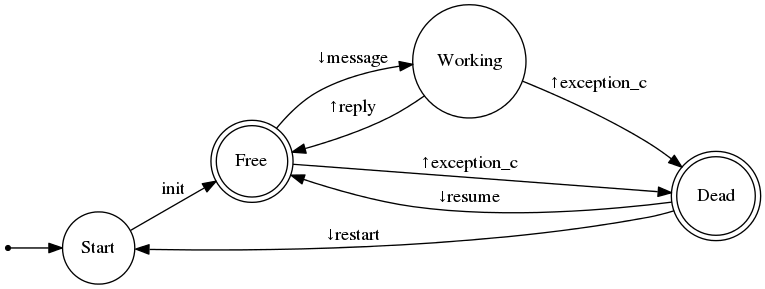
\includegraphics[scale=0.7]{child.png}
%            \caption{A gull}
            \label{fig:sup_node_1}
        }\\
        \subfigure[Supervisor]{
           \label{fig:sup_node_2}
           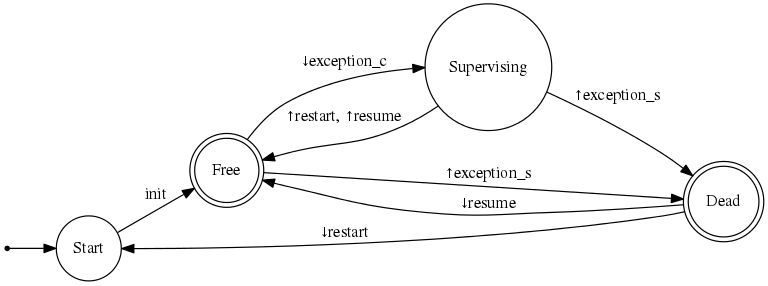
\includegraphics[scale=0.7]{supervisor.png}
        }\\
  \caption{Worker and Supervisor as Deterministic Finite Automata}
 \end{adjustwidth}      
  \label{fig:DFA}        
\end{figure}



Figure \ref{fig:DFA} gives the state graphs of DFAs that describe 
worker and supervisor in a supervision tree.  Nodes in the graphs represent 
states of that DFA and arrows are transitions from one state to another.  A 
transition is triggered either by the node itself or due to changes of the 
environment it resides.

At any time, a worker may be in one of its four states: {\bf Start}, {\bf 
Free}, {\bf Working}, or {\bf Dead}.  After automatically being initialized to 
the {\bf Free} state, the worker can receive a messages from its outside 
environment and enters into the {\bf Working} state where no other messages 
will be processed.  If no error occurred when processing the message, the 
worker returns a result and go back to the {\bf Free} state.  An error may 
occur during the middle of message processing (e.g. software bugs) or when the 
environment changes (e.g. hardware failures), in which cases the worker reports 
its failure to its supervisor and goes to the {\bf Dead} state.  A dead worker 
can be resumed (with the restored internal state) or restarted (with an initial 
internal state) by its supervisor so that it can process new messages.  The 
{\bf Free} and {\bf Dead} states are marked as accept states from which no 
further actions may occur.  On the contrary, a {\bf Working} worker will 
eventually emit a reply message or raise an exception; and all workers will be 
successfully initialized.

Similarly, Figure \ref{fig:sup_node_2} gives the DFA of a supervisor whose only 
duty is supervising its children.  A supervisor that in its {\bf Free} state 
reacts to failure messages from its children.  Meanwhile, a supervisor may fail 
at any time and reports its failure to its supervisor.

\subsection{The Supervision Relationship and Supervisor Strategies}
\label{supevision_tree_model}

\begin{figure}[h]
 \label{supevision_tree_fig} 
 \begin{tabular}{r c l l l}
 SupTree & =   & Worker &&\\
         & $|$ & OneForOne$_D$  & Sup & [SupTree] \\
         & $|$ & OneForAll$_D$  & Sup & [SupTree] \\
         & $|$ & RestForOne$_D$ & Sup & [SupTree] \\
         & $|$ & $\cdots$ &&\\
\\
 D & = & \multicolumn{3}{c}{Escalate $|$ Restart $|$ Resume $|$ 
Stop $|$ $\cdots$ } \\
         
 \end{tabular}
 \caption{Supervision Tree}
\end{figure}

The structure of a supervision tree is straightforwardly defined in Figure 
\ref{supevision_tree_fig}.  Each internal node is labelled by a supervisor 
strategy which contains a behaviour function whose type is {\tt Exception 
$\Rightarrow$ Directive}, where {\tt Exception} is the type of failures raised 
by children and {\tt Directive} represents the final {\tt system action} for 
that failure.  Subtrees of a node is organized as a List.

There are 3 general supervisor strategies found in existing libraries: {\tt 
OneForOne}, {\tt AllForOne}, and {\tt RestForOne}.  If a supervisor adopts the
{\tt OneForOne} strategy, the behaviour function is applied to the failed child 
only. If a supervisor adopts the {\tt AllForOne} supervisor strategy, the 
behaviour function is applied to all children when any of them fails.  If a 
supervisor adopts the {\tt RestForOne} supervisor strategy, the behaviour 
function is applied to the failed child and children in the rest of the list.  
New supervisor strategies can be added to the model when required.

The Erlang OTP library \citep{OTP} implements all three supervisor strategies 
whereas the Akka library \citep{akka_api, akka_doc} does not implement the {\tt 
RestForOne} strategy because children in Akka is not ordered.  Simulating the 
{\tt RestForOne} supervisor strategy in Akka requires ad-hoc implementation 
that groups related children and defines special messages to trigger actor 
termination.  No evidence shows that the lack of the {\tt RestForOne} 
strategy will result in difficulties when rewriting Erlang applications in Akka.

There are 4 directives found in existing libraries: {\tt Escalate}, {\tt 
Restart}, {\tt Resume}, and {\tt Stop}.  The {\tt Escalate} directive throws 
the exception to the supervisor of the supervisor; the {\tt Restart} directive 
restart the failed child with its initial internal state; the {\tt Resume} 
directive restart the failed child with the restored internal state and ask the 
child to process the message again; finally, the {\tt Stop} directive
terminates the failed actor permanently.  New directives can be added to the 
model when required.

The Akka library \citep{akka_api, akka_doc} implements all four directives 
whereas the Erlang OTP library \citep{OTP} only provides the {\tt Restart} 
directive and the {\tt Stop} directive.  The {\tt Escalate} directive can be 
simulated in Erlang by manually defining a function that terminates the 
supervisor when one of its children fails.  The {\tt Resume} directive is not 
needed in Erlang OTP because an Erlang actor does not have a mutable internal 
state.


\subsection{Unifying Supervisor and Worker}
\label{supervision_unifying}

\begin{figure}[p]
%  \ContinuedFloat 
\begin{adjustwidth}{-2.5cm}{} 
        \subfigure[Supervisor AND Worker]{
            \label{fig:sup_node_3}
            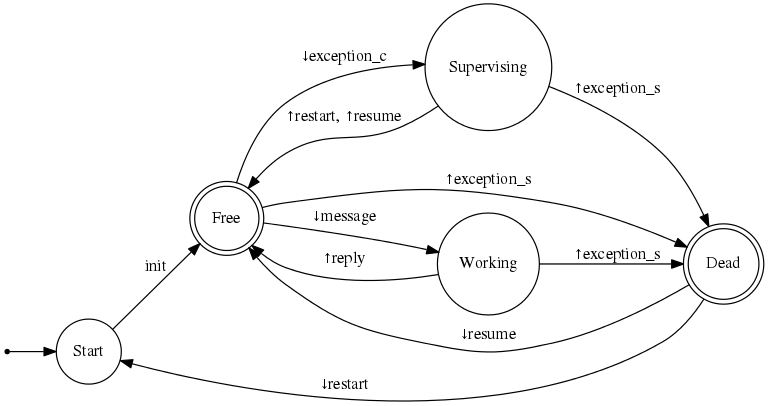
\includegraphics[scale=0.7]{supervisorANDchild.png}
        }\\
        \subfigure[Supervisor PAR Worker]{
            \label{fig:sup_node_4}
            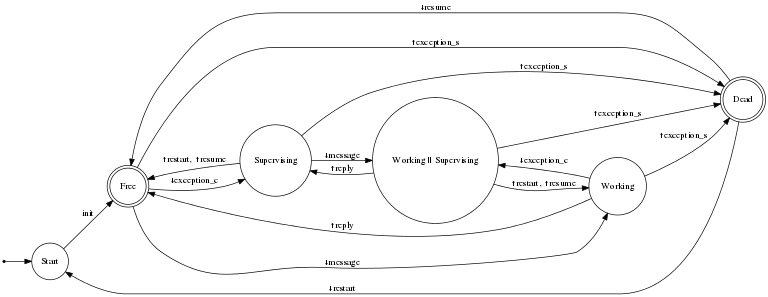
\includegraphics[scale=0.7]{supervisorPARchild.png}
        }\\
    \caption{A Node that Unifies Supervisor and Worker}
 \end{adjustwidth}    
   \label{fig:unify}
\end{figure}

Notice that the model for supervisor and worker are similar.  Can we define 
a {\it unified} model that matches both supervisor and worker?  Of course we 
can, and indeed there are three ways to do so.  This section will present three 
unified models and discuss the trade-off of using those models.

\paragraph{A General Actor Model}
The model for worker in Figure \ref{fig:sup_node_1} is no more than an actor 
that can be resumed or restarted when it fails.  If an exception raised from a 
child is viewed as a request message to its supervisor and a restart/resume 
command is viewed as a reply message to the child, the supervisor model (Figure 
\ref{fig:sup_node_2}) coincides with the worker model (Figure 
\ref{fig:sup_node_1}).  For this reason, in Erlang and Akka, both supervisors 
and workers are implemented as actors.  Defining supervisors and workers in 
terms of the general actor model is a reasonable implementation strategy; 
however, a specialized model for supervisor is desired in model analyses so 
that properties and behaviours of supervisors can be better discussed.

\paragraph{Combining Supervisor and Worker}  

The supervision tree defined in Section \ref{supevision_tree_model} requires 
supervisors as its internal nodes and workers as its leaves.  In contrast, the 
Akka library adopts the alternative design where an internal node can be both a 
supervisor for other nodes and a worker that implements part of the business 
logic.  The supervisor process and the worker process in Akka share the message 
box and are compounded to the message handler of the actor.  Figure 
\ref{fig:sup_node_3} gives a DFA that models the internal node of an Akka 
supervision tree.  It is clear that the internal node cannot restart or resume 
failed child when it is processing a message for other purposes, and it cannot 
perform a computational task when it carries out its duty as a supervisor.  In 
both cases, the performance of the system suffers.

\paragraph{Supervisor in Parallel with Worker}  One way to get around the 
limitation of the above design is executing the supervision process and the 
worker process in parallel, as shown in Figure \ref{fig:sup_node_4}.  
From the perspective of model analysis, the above parallel model is equivalent 
to the one which separates the supervisor process and the worker process into 
two nodes, and treat them either as siblings or as a supervisor and a child.  
Of course additional dependencies of the life cycle of those two logically 
separated nodes shall be addressed in the sense that the failure of one node 
will cause the failure of the other.

\vspace{15 pt}

To summarize, a node that naively combining the role of supervisor and worker 
(Figure \ref{fig:sup_node_3}) has less availability than a node that place the 
supervision process and the worker process in parallel (Figure 
\ref{fig:sup_node_4}).  Interestingly, during the process of designing and 
implementing the TAkka library (Chapter \ref{takka_design}), we realized that 
the type of supervision messages should be separated 
from the type of other messages.  However, partly because we would like to 
reuse the Akka implementation and partly because we did not have the above 
model at that time, the process of handling supervision messages is not 
separated from the process of handling other messages.


\subsection{Implementation Considerations}
\label{supervision_implementaion}

The two DFAs given in Figure \ref{fig:DFA} are abstracted for model analyses.  
In an implementation of the supervision tree model, following issues might be 
considered.

\paragraph{Distributed Deployment}
Supervision Tree represents the logic relationship between nodes.  In 
practice, nodes of a supervision tree may be deployed in distributed machines.  
A child node may be restarted at or shipped to another physical or virtual 
machine but stays in the same local position of the supervision tree.


\paragraph{Heart-Beat Message}  At run-time, failures may occur at any time 
for different reasons.  In some circumstances, failure messages of a child may 
not be delivered to its supervisor, or even worse, not be sent by the failed 
child at all.  To build a system tolerant to the above failures, supervisors 
need to be aware of the liveness of their children.  One commonly used approach 
is asking the child to periodically send heart-beat messages to 
its supervisor.  If no heart-beat message is received from a child within a 
time-out, that child is considered dead by the supervisor and an appropriate 
recovery process is activated.  In our model, a logical exception is sent from a 
child to its supervisor when no heart-beat message is delivered within a 
time-out, and a restart or resume message is sent to a suitable (virtual) 
machine where the recovered node will reside.

\paragraph{Message Queuing}
In the model given in Figure \ref{fig:sup_node_1}, a node can processed one 
message a time when it is {\bf Free}.  The model does not exclude the case 
where messages are queuing either in memory or a distributed database.  
Similarly, when a node is resumed from a failure, the message it was processing 
before that failure may either be restored or be discarded.


\section{Akka Basics}

\subsection{Akka Actor}
\label{akka actor}


An Akka Actor has four essential components as shown in Figure 
\ref{fig:akka_actor_api}: (i) a receive function that defines its reaction to 
incoming messages, (ii) an actor reference pointing to  itself, (iii) the actor 
 context representing the outside world of the actor, and (iv) the supervisor 
strategy for its children.

\begin{figure}[h]
\label{fig:akka_actor_api}
\begin{lstlisting}[language=scala]
package akka.actor
trait Actor{
  def receive:Any=>Unit
  val self:ActorRef
  val context:ActorContext
  var supervisorStrategy: SupervisorStrategy
}
\end{lstlisting}
\caption{Akka Actor API}
\end{figure}

Figure \ref{akkastring} shows an example actor in Akka.  The {\tt receive} 
function of the Akka actor has type {\tt Any$\Rightarrow$Unit} but the 
defined actor, {\tt ServerActor}, is only intended to process strings.  At Line 
16, a {\tt Props}, an abstraction of actor creation, is initialized and passed 
to an actor system, which creates an actor with name \textcolor{mauve}{\tt 
server} and returns a reference pointing to that actor.  Another way to obtain 
an actor is using the {\tt actorFor} method as shown in line 24.  We then use 
actor references to send the actor string messages and integer messages.  
String messages are processed in the way defined by the receive function.

\begin{figure}[p]
 \label{akkastring}
      \begin{lstlisting}[language=scala]
class ServerActor extends Actor {
  def receive = {
    case m:String => println("received message: "+m)
  }
}

class MessageHandler(system: ActorSystem) extends Actor {
  def receive = {
    case akka.actor.UnhandledMessage(message, sender, recipient) =>
      println("unhandled message:"+message);
  }
}

object ServerTest extends App {
  val system = ActorSystem("ServerTest")
  val server = system.actorOf(Props[ServerActor], "server")
  
  val handler = system.actorOf(Props(new MessageHandler(system)))
  system.eventStream.subscribe(handler,
                     classOf[akka.actor.UnhandledMessage]);
  server ! "Hello World"
  server ! 3
  
  val serverRef = system.actorFor("akka://ServerTest/user/server")
  serverRef ! "Hello World"
  serverRef ! 3
}


/*
Terminal output:
received message: Hello World
unhandled message:3
received message: Hello World
unhandled message:3
*/
    \end{lstlisting}
    \caption{A String Processor in Akka}
\end{figure}

Undefined messages are treated differently in different actor libraries.  In
Erlang, an actor keeps undefined messages in its mailbox, attempts to process
the message again when a new message handler is in use.  In versions prior to
2.0, an Akka actor raises an exception when it processes an undefined message.
In recent Akka versions, an undefined message is discarded by the actor and an
{\tt UnhandledMessage} event is pushed to the event stream of the actor system.
The event stream may be subscribed by other actors who are interested in
particular event messages.  To handle the unexpected integer message in the
above short example, an event handler is defined and created with 6 lines of 
code.


\subsection{Supervision}
\label{akkasup}

The Supervision Tree principle is proposed but optional in Erlang.  On the contrary,
the Akka library makes supervision obligatory by restricting the way of 
creating actors. Actors can only be initialized by using the {\tt actorOf}
method provided by {\tt ActorSystem} or {\tt ActorContext}.  Each actor system
provides a guardian actor for all user-created actors.  Calling the {\tt
actorOf} method of an actor system creates an actor supervised by the 
guardian actor.  Calling the {\tt actorOf} method of an actor context 
creates a child actor supervised by that actor.  Therefore, all user-created  
actors in an actor system, together with the guardian actor of that actor 
system, form a tree structure.  Obligatory supervision unifies the 
structure of actor deployment and simplifies the work of system maintenance.

Each actor in Akka is associated with an actor path.  The string representation
of the actor path of a guardian actor has format 
{\it akka://mysystem@IP:port/user}, where {\it mysystem} is the name of the 
actor system, {\it IP} and {\it port} are the IP address and the 
port number which the actor system listens to, and {\it user} is the name of 
the guardian actor.  The actor path of a child actor is actor path of its 
supervisor appended by the name of the child actor, either a user specified 
name or a system generated name.

Figure \ref{supervisedcalculator} defines a simple calculator which supports
multiplication and division. The simple calculator does not consider the
problematic case of dividing a number by 0, where an {\tt
ArithmeticException} will be raised.  We then define a safe calculator as the 
supervisor of the simple calculator.  The safe calculator delegates 
calculation tasks to the simple calculator and restarts the simple calculator 
when an {\tt ArithmeticException} is raised.  The supervisor strategy of
the safe calculator also specifies the maximum number of failures its child may 
have within a given time range.  If the child fails more frequently than the 
allowed frequency, the safe calculator will be  stopped, and its failure will be
reported to its supervisor, the system guardian actor in this example.  The
terminal output shows that the simple calculator is restarted before the third 
message and the fifth message are delivered.  The last message is not processed
because both calculators are terminated since the simple calculator fails more 
frequently than allowed.

\begin{figure}[p]
\label{supervisedcalculator}

  \begin{lstlisting}[language=scala]
case class Multiplication(m:Int, n:Int)
case class Division(m:Int, n:Int)

class Calculator extends Actor {
  def receive = {
    case Multiplication(m:Int, n:Int) =>
      println(m +" * "+ n +" = "+ (m*n))
    case Division(m:Int, n:Int) =>
      println(m +" / "+ n +" = "+ (m/n))
  }
}
class SafeCalculator extends Actor {
  override val supervisorStrategy =
    OneForOneStrategy(maxNrOfRetries = 2, withinTimeRange = 1 minute) {
      case _: ArithmeticException  =>
        println("ArithmeticException Raised to: "+self)
        Restart
    }
  val child:ActorRef = context.actorOf(Props[Calculator], "child")
  def receive = {    case m => child ! m  }
}
  val system = ActorSystem("MySystem")
  val actorRef:ActorRef = system.actorOf(Props[SafeCalculator],
"safecalculator")

  calculator ! Multiplication(3, 1)
  calculator ! Division(10, 0)
  calculator ! Division(10, 5)
  calculator ! Division(10, 0)
  calculator ! Multiplication(3, 2)
  calculator ! Division(10, 0)
  calculator ! Multiplication(3, 3)
/* Terminal Output:
3 * 1 = 3
java.lang.ArithmeticException: / by zero
ArithmeticException Raised to: Actor[akka://MySystem/user/safecalculator]
10 / 5 = 2
java.lang.ArithmeticException: / by zero
ArithmeticException Raised to: Actor[akka://MySystem/user/safecalculator]
java.lang.ArithmeticException: / by zero
3 * 2 = 6
ArithmeticException Raised to: Actor[akka://MySystem/user/safecalculator]
java.lang.ArithmeticException: / by zero
*/
    \end{lstlisting}
  \caption{Supervised Calculator}
\end{figure}




\begin{comment}
\section{Mixing Static and Dynamic Type Checking}
\label{type_checking}
A key advantages of static typing is that it detects some type errors at an 
early stage, i.e. at compile time.  The TAkka library is designed to detect 
type errors as early as possible.  Nevertheless, not all type errors can be 
statically detected, and some dynamic type checks are required. To address this 
issue, a notion of run-time type descriptor is required.

This section summarizes the type reflection mechanism in Scala and  explains
how it benefits the implementation of our typed name
server.  Our typed name server can be straightforwardly ported
to other platforms that support type reflection.

\subsection{Scala Type Descriptors}
Scala 2.8 defines a {\tt Manifest} class \footnote{Scala 2.10 introduces 
the Type class and the TypeTag class to replace Manifest.  At the time of this 
writing, TypeTag is not serializable as it should be due to bug SI-5919. } 
whose 
instance is a first class type descriptor used at runtime.  With the help of 
the {\tt Manifest} class, users can record the type information, including 
generic types, which may be erased by the JAVA compiler.  

In the Scala interactive session below, we obtain a Manifest value at Line 5 
and 
test a subtype relationship at Line 8.  To define a method that obtains type 
information of a generic type, Scala requires a type tag as an implicit 
argument to the method.  To simplify the API, Scala further provides a form of
syntactic sugar called context bounds.  We define a method using context
bounds at Line 11, which is compiled to the version using implicit 
arguments as shown at Line 12.


\begin{lstlisting}
scala> class Sup; class Sub extends Sup
defined class Sup
defined class Sub

scala> manifest[Sub]
res0: Manifest[Sub] = Sub

scala> manifest[Sub] <:< manifest[Sup]
res1: Boolean = true

scala> def getType[T:Manifest] = {manifest[T]}
getType: [T](implicit evidence$1: Manifest[T])Manifest[T]

scala> getType[Sub => Sup => Int]
res2: Manifest[Sub => (Sup => Int)] = scala.Function1[Sub, scala.Function1[Sup, 
Int]]

\end{lstlisting}


\subsection{Typed Name Server}
\label{nameserver}

In distributed systems, a name server maps each registered name, usually a
unique string, to a dynamically typed value, and provides a function to look up 
a value for a
given name. A name can be encoded as a {\tt Symbol} in Scala so that names
which represent the same string have the same value.  As a value retrieved from 
a name server is {\it dynamically typed}, it needs to be checked against and be 
cast to the expected type at the client side before using it.

To overcome the limitations of the untyped name server, we design and implement
a typed name server which maps each registered typed name to a value of the
corresponding type, and allows to look up a value by giving a typed name.

A typed name, {\tt TSymbol}, is a name shipped with a type descriptor.  A 
typed value, {\tt TValue}, is a value shipped with a type descriptor, which
describes a super type of the most precise type of that value.  
In Scala, {\tt TSymbol} and {\tt TValue} can be simply defined as in Figure
\ref{tsymbol}:

\begin{figure}[h]
\label{tsymbol}
\begin{lstlisting}
case class TSymbol[-T:Manifest](val s:Symbol) {
    private [takka] val t:Manifest[_] = manifest[T]
    override def hashCode():Int = s.hashCode()  
}

case class TValue[T:Manifest](val value:T){
  private [takka] val t:Manifest[_] = manifest[T]
}
\end{lstlisting}
\caption{TSymbol and TValue}
\end{figure}

{\tt TSymbol} is declared as a {\it case class} in Scala so that it can be 
used as a data constructor and for pattern matching.  In addition, the
type descriptor, {\tt t}, is constructed automatically and is private to the
{\tt takka} package so that only the library developer can access it as a field 
 
of {\tt TSymbol}. {\tt TValue} is declared as a {\it case class} for the same 
reason.

With the help of {\tt TSymbol}, {\tt TValue}, and a hashmap, a typed name 
server provides the following three operations:
\begin{itemize}
  \item {\tt set[T:Manifest](name:TSymbol[T], value:T):Boolean}

The {\tt set} operation registers a typed name with a value of corresponding 
type and returns true if the symbol representation of $name$ has not been
registered; otherwise the typed name server discards the request and
returns false.


  \item {\tt unset[T](name:TSymbol[T]):Boolean}

The {\tt unset} operation cancels the entry $name$ and returns true if (i) its 
symbol representation is registered and (ii) the type {\tt T} is a supertype of 
the registered type; otherwise the operation returns false.

  \item {\tt get[T] (name: TSymbol[T]): Option[T]}

The {\tt get} operation returns Some(v:{\tt T}), where {\tt v} is the value 
associated with {\tt name}, if (i) $name$ is associated with a value and (ii) 
{\tt T} is a supertype of the registered type; otherwise the operation returns 
None.
\end{itemize}

Notice that {\tt unset} and {\tt get} operations succeed as long as the 
associated type of the input name is the supertype of the associated type of 
the registered name.  To permit polymorphism, the {\tt hashcode} method of {\tt 
TSymbol} defined in  Figure {\ref{tsymbol}} does not take type values into 
account.  Equivalence comparison on {\tt TSymbol} instances, however, should 
consider the type.  Although the notion of {\tt TValue} does not appear in the
API, it is required for an efficient library implementation because the type 
information in {\tt TSymbol} is ignored in the hashmap.  Overriding the
hash function of {\tt TSymbol} also prevents the case where users accidentally
register two typed names with the same symbol but different types,
in which case if one type is a supertype of the other, the return value of
{\tt get} can be non-deterministic.  Last but not least, when an operation 
fails, the name server returns {\tt false} or {\tt None} rather than raising an
exception so that it is always available.

In general, dynamic type checking can be carried out in two ways.  The first 
method is to check whether the most precise type of a value conforms to the
structure of a data type.  Examples of this method include dynamically typed
languages and the {\tt instanceof} method in JAVA and other languages.  The
second method is to compare two type descriptors at run time.  The
implementation of our typed name server employs the second method because  
it detects type errors which may otherwise be left out.  Our
implementation requires the runtime type reification feature provided by Scala.
In a system that does not have such a feature, implementing typed name servers
is more difficult.


\end{comment}
 \chapter{Background and Related Work}
\label{background}

This chapter summarises work that influences the design and implementation of 
the TAkka library.  It begins with a general introduction on the 
Actor programming model (Section~\ref{actor_general}) and the Supervision principle
(Section~\ref{supervision_principle}), then explains OTP design 
principles in Erlang (Section~\ref{erlang_otp}), followed by a short tutorial on how to use the Actor 
programming model and the Supervision principle in the Akka library (Section~\ref{akka_lib}).  The 
Chapter concludes with a summary of features of the Scala type system used in the TAkka 
implementation (Section~\ref{scala_essence}).  The Actor model makes concurrent programming easy.  The 
Supervision principle makes applications robust.  The Supervision principle is 
introduced in the Erlang language.  It is obligatory in the Akka library, 
which is implemented in the Scala language.  Scala has a sophisticated type 
system, which enabled the experimental building of the more powerful and 
easier-to-use library, TAkka.


\section{The Actor Programming Model}
\label{actor_general}

The Actor Programming Model was first proposed by \citet{Hewitt:1973} for the 
purpose of constructing concurrent systems.  In the model, a concurrent system
consists of actors which are primitive computational components. Actors 
communicate with each other by sending messages.  Each actor independently 
reacts to messages it receives.

The Actor model given in \citep{Hewitt:1973} does not specify its formal 
semantics and hence does not suggest implementation strategies either.  An 
operational semantics of the Actor model is developed by 
\citet{actor_operational_semantics}.  \citet{acot_laws} later define a set of 
axiomatic laws for Actor systems.  Other semantics of the Actor model include 
the denotational semantics given by \citet{actor_denotational_semantics} and 
the transition-based semantic model by \citet{actor_transition_semantic}.
Meanwhile, the Actor model has been implemented in Act 1 \citep{Act1}, a 
prototype programming language.  The model influences designs of 
Concurrency Oriented Programming Languages (COPLs), especially the Erlang 
programming language \citep{ArmstrongErlang}, which has been used in 
enterprise-level applications since it was developed in 1986.
  
A recent trend is adding actor libraries to full-fledged popular programming 
languages that do not have actors built-in.  Some of the recent actor libraries 
are JActor  \citep{JActor} for the JAVA language, Scala Actor \citep{actor_1, 
actor_2} for Scala, Akka \citep{akka_doc} for Java and Scala, and CloudHaskell 
\citep{CloudHaskell} for Haskell.


\section{The Supervision Principle}
\label{supervision_principle}

The core idea of the supervision principle is that actors should 
be monitored and restarted when necessary by their supervisors in order to 
improve the availability of a software system.  The supervision principle was 
first proposed in the Erlang/OTP library \citep{OTP} and was adopted by the Akka 
library \citep{akka_doc}.

A supervision tree in Erlang consists of two types of actors: workers and 
supervisors. A worker implements part of the business logic and reacts to 
request messages.  A supervisor is responsible for initializing and monitoring 
its children, which are workers or supervisors for other actors, and restarting 
its children when necessary.  The behaviour of a supervisor is defined by its 
{\it supervision strategy}.

The Akka library makes supervision obligatory.  In Akka, every user-created 
actor is either a child of the system guidance actor or a child of another 
user-created actor.  Therefore, every Akka actor is potentially the supervisor 
of some other actors.  Unlike the Erlang system, an Akka actor can be 
both a worker and a supervisor.





\section{Erlang and OTP Design Principles}
\label{erlang_otp}

Erlang \citep{erlang_history, ArmstrongErlang} is a dynamically typed 
functional programming language originally designed at the Ericsson Computer 
Science Laboratory for implementing telephony applications 
\citep{erlang_history}.  After using the Erlang language for in-house 
applications for ten years, when Erlang was released as open source in 1998, 
Erlang developers summarised five design principles shipped with the Erlang/OTP 
library, which stands for Erlang Open Telecom Platform \citep{erlang_history, 
OTP}.

Erlang provides fault-tolerant support for many enterprise-level distributed real-time
applications, which often contain components implemented using other languages.
One of the early OTP 
applications, Ericsson's AXD 301 switch, is reported to have achieved nine 9s 
availability, that is, 99.9999999\% of uptime, during its nine-month experiment 
\citep{ArmstrongAXD}.  Up to the present day, Erlang has been widely used in 
database systems (e.g. Mnesia, Riak, and Amazon SimpleDB) and messaging 
services (e.g. RabbitMQ and WhatsApp).


The five OTP design principles are: The Behaviour 
Principle, The Application Principle, The Release Principle, The Release 
Handling Principle, and The Supervision Principle \citep{OTP}.  The Supervision Principle 
was introduced in the previous section.  This section describes the ideas 
of the remaining 4 OTP design principles and the methodology of applying them 
in a JVM based environment, such as Java and Scala.  The Supervision principle, 
which is the central topic of this thesis, has no direct correspondence in 
general Java and Scala programming practice.



\subsection{The Behaviour Principle}

A Behaviour in Erlang is similar to an interface, a trait, or an abstract class
in object oriented programming.  It defines common structures and patterns of 
process implementations.  With the help of behaviours, Erlang code can be 
divided into a generic part (a behaviour module) and a specific part (a 
callback module).  Most Erlang processes, including those in the Erlang standard library,  are 
coded by implementing a set of pre-defined callback functions for one or 
more behaviours.  Although ad-hoc code and programming structures may be more 
efficient, using consistent general interfaces makes code more maintainable and 
reliable.  
\begin{comment}
Standard Erlang/OTP behaviours include: 

\begin{itemize} 
  \item $\it{gen\_server}$  for constructing the server of a client-server 
paradigm. 
  \item $\it{gen\_fsm}$ for constructing finite state machines. 
  \item $\it{gen\_event}$ for implementing event handling functionality. 
  \item $\it{supervisor}$ for implementing a supervisor in a supervision tree. 
\end{itemize}
\end{comment}

\newpage
\subsection{The Application Principle}

A software system on the OTP platform is made up of a group of components 
called applications.  To define an application, users implement two callback 
functions of the {\tt application} behaviour: {\tt start/2} and {\tt stop/1}.
In Erlang API, the signature of a function contains its name and the number
of arguments it takes.  Because Erlang is dynamically typed, users of an Erlang
library need to study the type of each function from respected documentation.
Applications without any processes are called library applications.  
In an Erlang runtime system, all operations on applications are managed by the 
$\it{application\ controller}$ process, registered as {\tt application\_controller}.

Distributed applications may be deployed on several distributed Erlang nodes.  
An Erlang distributed application will be restarted at another node when its 
current node goes down.  A distributed application is controlled by both the 
application controller and the distributed application controller, registered as 
{\tt dist\_ac}, both of which are part of the $\it{kernel}$  
application.  Two configuration parameters must be set before loading and 
launching a distributed application.  First, possible nodes where the 
distributed application may run must be explicitly pointed.  Second, all nodes 
configured in the last step will be sent a copy of the same configuration which 
includes three parameters: the time for other nodes to start, nodes that {\it 
must} be started in a timeout, and nodes that {\it may} be started in a 
timeout.


\subsection{The Release Principle and The Release Handling Principle}

A complete Erlang system consists of one or more applications, packaged in a 
release resource file.  Different versions of a release can be upgraded or 
downgraded at run-time dynamically by calling API in the {\tt release\_handler} 
module in the SASL (System Architecture Support Libraries) application.  Hot 
swapping on an entire release application is a distinct feature of Erlang/OTP, 
which aims at designing and running non-stop applications.


\subsection{Applying OTP Design Principles in Java and Scala}

To sum up, Table~\ref{otp} summarises an analogy between Erlang/OTP 
design principles and common practices in Java and Scala programming.  

\begin{table}[h]
\begin{tabular}{| l | p{10 cm} | }
\hline
  OTP Design Principle & Java/Scala Analogy \\
\hline
  Behaviour & defining an abstract class, an interface, or a trait. \\
\hline
  Application  & defining an abstract class that has two abstract methods: start 
and stop, or using Java/Scala an equivalent class such as {\tt Thread}. \\
\hline
  Release  & packaging related application classes  \\ 
\hline
  Release Handling  & hot swapping support on key modules is required \\
\hline
  Supervision  & no direct correspondence  \\
\hline
\end{tabular}
 \caption[]{Using OTP Design Principles in JAVA and Scala Programming}
\label{otp}
\end{table}

First, the notion of callback functions in Erlang/OTP is close to that
of abstract methods in Java and Scala.  An OTP behaviour that only defines the 
signature of callback functions can be ported to Java and Scala as an interface. 
 An OTP behaviour that implements some behaviour functions can be ported as an 
abstract class to {\it prevent} multiple inheritance, or a trait to {\it permit} 
multiple inheritance.  Since Java does not have the notion of trait, porting an 
Erlang/OTP module that implements multiple behaviours requires a certain amount 
of refactoring work.

Second, since the Erlang application module is just a special behaviour, a 
programmer can 
define an equivalent interface {\tt Application} which contains two abstract 
methods: {\tt start} and {\tt stop}.  To mimic the dynamic type system of Erlang 
system, the {\tt start} method may be declared as \\ 
{\tt public static void start(String name, Object... arguments)}
and as \\  
{\tt def start(name:String, arguments:Any*):Unit} in Java and Scala 
respectively. 

Third, Erlang releases correspond to  packages in Java and Scala whereas hot 
code swapping is not directly supported by JVM.  During the development of the 
TAkka library, the author noticed that dynamically upgrading key components can 
be mimicked by updating the references to those components.

The final OTP design principle, Supervision, has no direct correspondence in 
Java and Scala programming practices.  The next section introduces the Akka 
library which implements the supervision principle.






\begin{comment}

\section{The Erlang Programming Language}

Erlang \citep{erlang_history, ArmstrongErlang} is a dynamically typed 
functional programming language originally designed at the Ericsson Computer 
Science Laboratory for implementing telephony applications 
\citep{erlang_history}.  After using the Erlang language for in-house 
applications for ten years, when Erlang was released as open source in 1998, 
Erlang developers summarised five design principles shipped with the Erlang/OTP 
library, which stands for Erlang Open Telecom Platform \citep{erlang_history, 
OTP}.

Erlang, collaborates with other languages, provides fault-tolerant support for 
enterprise-level distributed real-time applications. One of the early OTP 
applications, Ericsson’s AXD 301 switch, is reported to have achieved nine “9”s 
availability, that is 99.9999999\% of uptime, during the nine months experiment 
\citep{ArmstrongAXD}.  Up to the present, 
Erlang has been widely used in database systems (e.g. Mnesia, Riak, and Amazon 
SimpleDB) and messaging services (e.g. RabbitMQ and WhatsApp).

This section gives a brief introduction to the Erlang programming language and 
OTP design principles, based on related material in \citep{ArmstrongErlang} and 
\citep{ErlangManual, ErlangStart, OTP}.




\subsection{Actor Programming in Erlang}

(This section summarises material from \citep[Chapter 8]{ArmstrongErlang} and 
\citep[Chapter 3]{ErlangStart})

\vspace{12 pt}

An Erlang application consists of one or more module files, each of which 
defines a set of functions.  The notion of the Erlang {\it process} minimizes 
the gap between sequential programming and concurrent programming.  In Erlang, 
a process is a thread of function execution.  It can receive messages of any 
type via its process identifier (pid).  Defining an Actor in Erlang is as 
simple as providing a {\tt receive} block for the body of the function spawned 
in a process.


\subsubsection{Processes Creation}

A {\it process} in Erlang is a thread of function execution.  A process is 
created by calling the {\tt spawn} method.  Figure~\ref{erlang_spawn} gives the 
API of the {\tt spawn} method \citep{ErlangManual}.  Calling {\tt spawn(Module, 
Function, Args)} creates a process that executes the function {\tt 
Module:Function(Args)}, where {\tt Args} is a list of arguments.  The {\tt 
spawn} method returns a process identifier (pid) of the created process, which 
terminates when the execution of the function completes.

\begin{figure}[!h]

\begin{lstlisting}
spawn(Module, Function, Args) -> pid()

  Module = Function = atom()
  Args = [Arg1,...,ArgN]  
  ArgI = term()
\end{lstlisting}  
\caption{Erlang API: spawn}
\label{erlang_spawn}
\end{figure}

To demonstrate the creation and usage of Erlang processes, Figure 
\ref{erlang_echo} shows the {\tt echo} example modified from \citep[the {\tt 
tut14} module]{ErlangStart} and its test result.  As the terminal output shows, 
the {\tt say\_something} function prints out its first argument for the number 
of times specified by its second argument.  What is more interesting is the 
result of {\tt echo:start()}, which spawns two processes.  The result shows 
that the execution of the two processes and the main thread, which returns a 
pid of the last {\tt spawn} (i.e. {\tt <0.41.0>}), are in parallel.  As a 
consequence, the program prints out ``hello'', ``goodbye'', and the pid in a 
non-deterministic order.

\begin{figure}[!h]
\begin{lstlisting}
-module(echo).

-export([start/0, say_something/2]).

say_something(_, 0) ->
    done;
say_something(What, Times) ->
    io:format("~p~n", [What]),
    say_something(What, Times - 1).

start() ->
    spawn(echo, say_something, [hello, 3]),
    spawn(echo, say_something, [goodbye, 3]).

%% Terminal Output:
%% 1> c(echo).
%% {ok,echo}
%% 2> echo:say_something(hello, 3).
%% hello
%% hello
%% hello
%% done
%% 3> echo:start().
%% hello
%% goodbye
%% <0.41.0>
%% hello
%% goodbye
%% hello
%% goodbye  
\end{lstlisting}  
\caption{Erlang Example: An Echo Process}
\label{erlang_echo}
\end{figure}



\subsubsection{Message Passing Style Concurrency}
\label{erlang_message_passing}
In the {\tt echo} example, the two processes are executed independently.  To 
be an actor, an Erlang process shall be able to receive messages from others 
and reacts to messages.

In Erlang, users can send a message to a process via its pid using the {\tt !} 
primitive.  For example, the code 
\begin{lstlisting}
  Pid ! Msg
\end{lstlisting}
will send the message {\tt Msg} to the process whose pid is {\tt Pid}. Message 
sending is an asynchronous operation. Its evaluation result is the evaluated 
value of the sent message.

Messages sent to a process is queued in the mailbox of the recipient.  To 
handle a received message, a process provides a {\tt receive} block with the 
following syntax:

\begin{figure}[h]
\begin{lstlisting}
 receive
   Message1 [when Guard1] ->
     Action1 ;
   Message2 [when Guard2] ->
     Action2 ;
   ...
   MessageN [when GuardN] ->
     ActionN
 end
\end{lstlisting}
\caption{Erlang receive block}
\label{fig:ErlangReceiveAPI}
\end{figure}

In the Erlang code pattern given in Figure~\ref{fig:ErlangReceiveAPI}, {\tt 
receive} and {\tt end} are primitives that denote the scope of the receive 
block.  A receive block defines a set of guarded message patterns to which the 
current processed message will be matched in order. If the current message 
matches a pattern, the corresponding action will be evaluated.  If the current 
message does not match any pattern, it will be saved in the mailbox and the 
next message in the mailbox will be processed.  When reaching a receive block, 
the evaluation of the process will be suspended until at least one message in 
the mailbox matches one of the guarded patterns.  

Because messages may be concurrently sent from parallel threads or distributed 
nodes, the order in which messages appear in the mailbox 
is not necessarily the same as the order those messages were sent.  
Nevertheless, messages sent from the same sender to the same receiver is 
guaranteed to appear in the mailbox in the order they were sent, if both are 
delivered.     

The {\tt echo\_actor} example, given in Figure~\ref{fig:ErlangEchoActor}, 
spawns two processes, both of which verbatim print their received messages.  
The {\tt print} function terminates as soon as the first message is processed.  
On the contrary, {\tt loop} is a recursive function that can always process new
messages.  Line 34 of Figure~\ref{fig:ErlangEchoActor} confirms two properties 
of message sending in Erlang.  Firstly, message sending is always a successful 
operation that returns the value of the sent message.  At line 24, {\tt P} is a 
pid pointing to a terminated process.  Nevertheless, sending a message to {\tt 
P} is still permitted.  Secondly, message sending  is an asynchronous operation. 
 In this example, the evaluation result of line 23 is printed out after the 
evaluation result of the {\tt start} function (i.e. {\tt hello4}), probably 
because it takes some time to match the message sent in line 23.





\begin{figure}[!h]

\begin{lstlisting}
-module(echo_actor).

-export([start/0, loop/0, print/0]).

loop() ->
    receive
        Msg -> 
          io:format("loop: ~p~n", [Msg]),
          loop()
    end.

print() ->
    receive
        Msg -> 
          io:format("print: ~p~n", [Msg])
    end.
    
start() ->
    L = spawn(echo_actor, loop, []),
    P = spawn(echo_actor, print, []),
    L ! hello1,
    P ! hello2,
    L ! hello3,
    P ! hello4.


%% Terminal Output:

%% 1> c(echo_actor).     
%% {ok,echo_actor}
%% 2> echo_actor:start().
%% loop: hello1
%% print: hello2
%% hello4
%% loop: hello3


\end{lstlisting}
\caption{Erlang Example: An Echo Actor}
\label{fig:ErlangEchoActor}
\end{figure}


\subsubsection{An Erlang Actor with State}

Erlang is a functional programming language where the value of a variable is 
immutable once assigned.  On the other side, the result of a computation, for 
example, a search query, often depends on the value of some internal states.  
Therefore, an Erlang actor needs to retain or update its internal states when it
updates its behaviour.  One common method to define an Erlang actor with 
internal
state is passing the state to the behaviour function.  


The {\tt counter} example defined in Figure~\ref{fig:erlang_counter} has one 
state variable, {\tt Val}, which records the number of messages it has 
processed.  The internal state is initialized to 0 when the actor is 
created at line 5.  The value of the state is incremented each time when a 
message is processed (line 14 and line 17).

\begin{figure}[!h]


\begin{lstlisting}
-module(counter).
-export([start/0, counter/1]).
 
start() ->
    S = spawn(counter, counter, [0]),
    S ! increment,
    send_msgs(S, 3),
    S.
 
counter(Val) ->
    receive
        increment ->
          io:fwrite("increase counter to ~w~n", [Val+1]),
          counter(Val+1);
        Msg -> 
          io:fwrite("~w message(s) that has/have been processed ~n", [Val+1]),
          counter(Val+1)
    end.
 
send_msgs(_, 0) -> true;
send_msgs(S, Count) ->
    S ! "Hello",
    send_msgs(S, Count-1).
 
%% Terminal Output:
%% 1> c(counter).
%% {ok,counter}
%% 2> counter:start().
%% increase counter to 1
%% <0.95.0>
%% 2 message(s) has/have been processed 
%% 3 message(s) has/have been processed 
%% 4 message(s) has/have been processed
\end{lstlisting}
  \caption{Erlang Example: A Message Counter}
  \label{fig:erlang_counter}
\end{figure}



\subsection{Supervision in Erlang}
\label{erlang_supervision}

(This section summarises material from \citep[Chapter 5]{OTP})
\vspace{12 pt}

Supervision is probably the most important concept in the OTP design 
principles \citep{OTP}.  A supervision tree consists of workers and 
supervisors. Workers are processes which carry out actual computations while 
supervisors are processes which inspect a group of workers or sub-supervisors.  
Since both workers and supervisors are processes and they are organised in a 
tree structure, the term $\it{child}$ is used to refer to any supervised 
process.  The structure of a supervision tree may look like the 
one presented in Figure~\ref{fig:erlang_supervison_tree}, where supervisors are 
represented by squares and workers are represented  by circles.  The example is 
cited from \citep[Section 1.1]{OTP}.  Restart strategies of each supervisor 
(Section~\ref{erlang_supervision_strategy}), however, are 
removed from the figure since they are not related to the central ideas 
discussed at this moment.

\vspace{12 pt}

\begin{figure}[h]
\begin{center}

\begin{picture}(280, 250)
  \put(15, 70){\circle{30}}
  \put(95, 0){\circle{30}}
  \put(180, 0){\circle{30}}
  \put(260, 0){\circle{30}}
  
  \put(80,55){\line(0,1){30}}
  \put(80,85){\line(1,0){30}}
  \put(110,85){\line(0,-1){30}}
  \put(110,55){\line(-1,0){30}}
  
  \put(200,55){\line(0,1){30}}
  \put(200,85){\line(1,0){30}}
  \put(230,85){\line(0,-1){30}}
  \put(230,55){\line(-1,0){30}}
  
  \put(140,125){\line(0,1){30}}
  \put(140,155){\line(1,0){30}}
  \put(170,155){\line(0,-1){30}}
  \put(170,125){\line(-1,0){30}}
  
  \put(0,125){\line(0,1){30}}
  \put(0,155){\line(1,0){30}}
  \put(30,155){\line(0,-1){30}}
  \put(30,125){\line(-1,0){30}}  

  \put(70,202){\line(0,1){30}}
  \put(70,232){\line(1,0){30}}
  \put(100,232){\line(0,-1){30}}
  \put(100,202){\line(-1,0){30}}  

  \put(180,15){\line(1,1){40}}
  \put(260,15){\line(-1,1){40}}
  \put(95,15){\line(0,1){40}}
  
  \put(95,85){\line(3,2){62}}
  \put(220,85){\line(-3,2){62}}
  \put(15,85){\line(0,1){40}}
  
  \put(15,155){\line(3,2){70}}
  \put(155,155){\line(-3,2){70}}
\end{picture}

\end{center}
\caption{A Supervision Tree}
\label{fig:erlang_supervison_tree}
\end{figure}

\newpage

\subsubsection{An Erlang Supervision Example}

We present the code for a simple Erlang supervisor in Figure 
\ref{erlang_supervision_demo}.  The core computation of the {\tt 
supervision\_demo} example is a problematic function {\tt loop}, which 
eventually will try to compute the quotient of 10 divided by 0.  As the test 
result shows, the problematic process has been restarted twice when it raises 
an error.  The process is killed when it has failed for the third time within 
60 seconds.  

The short example implements the {\tt supervisor} behaviour and specifies its 
supervision policy in its {\tt init/1} method.  The supervision policy 
reads as the following: spawn a worker process by calling {\tt 
spawn(supervisor\_demo, start, [Count])}; always restart the child when it 
fails if it does not fail more than twice within 60 seconds; if the 
child process fails more frequently than allowed, terminate it immediately.  
Alternative Erlang supervision strategies are explained in the following.

\begin{figure}[p]

\begin{lstlisting}
-module(supervisor_demo).
-behaviour(supervisor).

-export([start/0, start/1, loop/1, init/1]).

start() ->
    supervisor:start_link(supervisor_demo, [2]).

start(Count) ->
  io:fwrite("Starting...~n"),
  Pid=spawn_link(supervisor_demo, loop, [Count]),
  {ok, Pid}.
	
init([Count]) ->
  {ok, {{one_for_one, 2, 60},
          [{supervisor_demo, {supervisor_demo, start, [Count]},
          permanent, brutal_kill, worker, [supervisor_demo]}]}}.
	
loop(Count) ->
  io:fwrite("~w / ~w is ~w ~n", [10, Count, 10/Count]),
  loop(Count-1).
  
%% 1> c(supervisor_demo).
%% {ok,supervisor_demo}
%% 2> supervisor_demo:start().
%% Starting...
%% 10 / 2 is 5.0 
%% 10 / 1 is 10.0 
%% <0.39.0>
%% Starting...
%% 10 / 2 is 5.0 
%% 10 / 1 is 10.0 
%% Starting...
%% 3> 
%% =ERROR REPORT==== 14-Oct-2013::00:03:49 ===
%% Error in process <0.40.0> with exit value: 
{badarith,[{supervisor_demo,loop,1,[{file,"supervisor_demo.erl"},{line,20}]}]}
%% 10 / 2 is 5.0 
%% 3> 
%% =ERROR REPORT==== 14-Oct-2013::00:03:49 ===
%% Error in process <0.42.0> with exit value: 
{badarith,[{supervisor_demo,loop,1,[{file,"supervisor_demo.erl"},{line,20}]}]}
%% 10 / 1 is 10.0 
%% =ERROR REPORT==== 14-Oct-2013::00:03:49 ===
%% Error in process <0.43.0> with exit value: 
{badarith,[{supervisor_demo,loop,1,[{file,"supervisor_demo.erl"},{line,20}]}]}
%% ** exception error: shutdown
\end{lstlisting}  
\caption{Erlang Example: Supervision Demo}
\label{erlang_supervision_demo}
\end{figure}




\subsubsection{Supervision Strategy}
\label{erlang_supervision_strategy}

In principle, a supervisor is accountable for starting, stopping and monitoring 
its child processes according to the policy specified in its {\tt init/1} 
method, according to the API given in Figure~\ref{erlang_supervision_api} 
\citep{OTP}.  A supervision strategy contains two parts: a restart strategy 
applies to all children and a list of child specifications for each child.

An Erlang supervisor employs one of the four restart strategies which specify 
its behaviour when one of its child fails.  A supervisor with {\tt 
one\_for\_one} strategy restarts a child when it fails.  A supervisor with {\tt 
one\_for\_all} strategy restarts all children when one of them fails.  A 
supervisor with {\tt rest\_for\_one} strategy restart the failed child and 
other children that started later than the failed child, according to their 
order in the list of child specifications.  A supervisor with 
{\tt simple\_one\_for\_one} strategy is a {\tt one\_for\_one} supervisor whose 
children are dynamically added instances of the same process.

A child specification contains 6 pieces of information \citep{OTP}: 
\begin{inparaenum} [i)]
  \item an internal name of the supervisor to identify the child. 
  \item the function call to start the child process.
  \item whether the child process should be restarted after the termination of 
its siblings or itself.
  \item how to terminate the child process.
  \item whether the child process is a worker or a supervisor.
  \item a singleton list which specifies the name of the callback module. 
\end{inparaenum}



\begin{figure}[p]

\begin{lstlisting}
Module:init(Args) -> Result

Args = term()
Result = {ok, {{RestartStrategy,MaxR,MaxT},[ChildSpec]}} | ignore
   RestartStrategy = strategy()
   MaxR = integer()>=0
   MaxT = integer()>0
   ChildSpec = child_spec()
   
child_spec() = 
    {Id :: child_id(),
     StartFunc :: mfargs(),
     Restart :: restart(),
     Shutdown :: shutdown(),
     Type :: worker(),
     Modules :: modules()}
     
child_id() = term()

mfargs() = 
    {M :: module(), F :: atom(), A :: [term()] | undefined}

restart() = permanent | transient | temporary

shutdown() = brutal_kill | timeout()

strategy() = one_for_all
           | one_for_one
           | rest_for_one
           | simple_one_for_one
               
worker() = worker | supervisor            

modules() = [module()] | dynamic

\end{lstlisting}  
\caption{Erlang API: supervision}
\label{erlang_supervision_api}
\end{figure}



\subsection{Other OTP Design Principles}

Based on 10 years of experience of using Erlang in Enterprise level 
applications, Erlang developers summarized 5 OTP design principles in 1999 to 
improve the reliability of Erlang applications \citep{OTP}: The Behaviour 
Principle, The Application Principle, The Release Principle, The Release 
Handling Principle, and The Supervision Principle.  The Supervision Principle 
has been introduced in the previous section.  This section describes the idea 
of the remaining 4 OTP design principles and the methodology of applying them 
in a JVM based environment, such as Java and Scala.  The Supervision principle, 
which is the central topic of this thesis, has no direct correspondence in 
general Java and Scala programming practice.

\subsubsection{The Behaviour Principle}

A Behaviour in Erlang is similar to an interface, a trait, or an abstract class
in the objected oriented programming.  It implements common structures and patterns of process 
implementations.  With the help of behaviours, Erlang code can be divided into a 
generic part, a behaviour module, and a specific part, a callback module.  Most 
processes, including the supervisor in Section~\ref{erlang_supervision}, is coded
by implementing a set of pre-defined callback functions for one or 
more behaviours.  Although ad-hoc code and programming structures may be more 
efficient, using consistent general interfaces make code more maintainable and 
reliable.  Standard Erlang/OTP behaviours include: 

\begin{itemize} 
  \item $\it{gen\_server}$  for constructing the server of a client\-server 
paradigm. 
  \item $\it{gen\_fsm}$ for constructing finite state machines. 
  \item $\it{gen\_event}$ for implementing event handling functionality. 
  \item $\it{supervisor}$ for implementing a supervisor in a supervision tree. 
\end{itemize}


\subsubsection{The Application Principle}

A software system on the OTP platform is made of a group of components called 
applications.  To define an application, users implements two callback 
functions of the {\tt application} behaviour: {\tt start/2} and {\tt stop/1}.  
Applications without any processes are called library applications.  
In an Erlang runtime system, all operations on applications are managed by the 
$\it{application\ controller}$ process, registered as {\tt application\_controller}.

Distributed applications may be deployed on several distributed Erlang nodes.  
An Erlang distributed application will be restarted at another node when its 
current node goes down.  A distributed application is controlled by both the 
application controller and the distributed application controller, registered as 
{\tt dist\_ac}, both of which are part of the $\it{kernel}$  
application.  Two configuration parameters must be set before loading and 
launching a distributed application.  First, possible nodes where the 
distributed application may run must be explicitly pointed.  Second, all nodes 
configured in the last step will be sent a copy of the same configuration which 
include three parameters: the time for other nodes to start, nodes that {\it 
must} be started in a given time, and nodes that {\it may} be started in a 
given time.


\subsubsection{The Release Principle and The Release Handling Principle}

A complete Erlang system consists of one or more applications, packaged in a 
release resource file.  Different version of a release can be upgraded or 
downgraded at run-time dynamically by calling API in the {\tt release\_handler} 
module in the SASL (System Architecture Support Libraries) application.  Hot 
swapping on an entire release application is a distinct feature of Erlang/OTP, 
which aims at design and running non-stop applications.


\subsubsection{Appling OTP Design Principles in Java and Scala}

To sum, we make an analogy between Erlang/OTP design principles and common 
practices in Java and Scala programming, summarised in Table~\ref{otp}.  

\begin{table}[h]
\begin{tabular}{| l | p{10 cm} | }
\hline
  OTP Design Principle & Java/Scala Analogy \\
\hline
  Behaviour & defining an abstract class, an interface, or a trait. \\
\hline
  Application  & defining an abstract class that has two abstract methods: start 
and stop \\
\hline
  Release  & packaging related application classes  \\ 
\hline
  Release Handling  & hot swapping support on key modules is required \\
\hline
  Supervision  & no direct correspondence  \\
\hline
\end{tabular}
 \caption[]{Using OTP Design Principles in JAVA and Scala Programming}
\label{otp}
\end{table}

First, the notion of callback functions in Erlang/OTP is close to the notion 
of abstract methods in Java and Scala.  An OTP behaviour that only defines the 
signature of callback functions can be ported to Java and Scala as an interface. 
 An OTP behaviour that implements some behaviour functions can be ported as an 
abstract class to {\it prevent} multiple inheritance, or a trait to {\it permit} 
multiple inheritance.  Since Java does not have the notion of trait, porting an 
Erlang/OTP module that implements multiple behaviours requires a certain amount 
of refactoring work.

Second, since the Erlang application module is just a special behaviour, we can 
define an equivalent interface {\tt Application} which contains two abstract 
methods: {\tt start} and {\tt stop}.  To mimic the dynamic type system of Erlang 
system, the {\tt start} method may be declared as \\{\tt public static void 
start(String name, Object... arguments)}  and as \\  
{\tt def start(name:String, arguments:Any*):Unit} in Java and Scala 
respectively. 

Third, Erlang releases correspond to  packages in Java and Scala whereas hot 
code 
swapping is not directly supported by JVM.  During the development of the TAkka 
library, we noticed that hot code swapping on a key component can be mimicked 
by updating the reference to that component.

The final OTP design principle, Supervision, has no direct correspondence in 
Java and Scala programming practices.  The next section introduces the Akka 
library which implements the supervision principle.


\end{comment}




\section{The Akka Library}
\label{akka_lib}

Akka is a Scala library that enforces the supervision principle.  The next section briefly
introduces Scala features that used in this thesis.  The API of the 
Akka library \citep{akka_api, akka_doc} is similar to the Scala 
Actor library \citep{actor_1, actor_2}, which borrows syntax from the Erlang 
languages \citep{ArmstrongErlang, ErlangManual}.  Both Akka and Scala Actor are 
built in Scala, a typed language that merges features from Object-Oriented 
Programming and Functional Programming.  This section gives a brief tutorial 
on Akka, based on related materials in the Akka Documentation 
\citep{akka_doc}.  The Akka API used in this thesis is listed in Figure A.1, Appendix A.


\subsection{Actor Programming in Akka}
\label{subsection:actor_akka}

(This section summarises material from \citep[Section 2.3 and 3.1]{akka_doc})
\vspace{12 pt}

Although many Akka designs have their origin in Erlang, the Akka Team at 
Typesafe Inc. devises a set of connected concepts that explains Actor 
programming in the Akka framework.  This subsection begins with a short Akka 
example, followed by elaborate explanations of involved concepts.



\begin{figure}[p]
      \begin{lstlisting}[language=scala]
package sample.akka

import akka.actor.{Actor, ActorRef, ActorSystem, Props}
      
class StringCounter extends Actor {
  var counter = 0;
  def receive = {
    case m:String => 
      counter = counter +1
      println("received "+counter+" message(s):\n\t"+m)
  }
}

class MessageHandler extends Actor {
  def receive = {
    case akka.actor.UnhandledMessage(message, sender, recipient) =>
      println("unhandled message:"+message);
  }
}

object StringCounterTest extends App {
  val system = ActorSystem("StringCounterTest")
  val counter = system.actorOf(Props[StringCounter], "counter")
  
  val handler = system.actorOf(Props[MessageHandler]))
  system.eventStream.subscribe(handler,classOf[akka.actor.UnhandledMessage]);
  counter ! "Hello World"
  counter ! 1
  Thread.sleep(1000)
  val counterRef = system.actorFor("akka://StringCounterTest/user/counter")
  counterRef ! "Hello World Again"
  counterRef ! 2
}


/*
Terminal output:
received 1 message(s):
	Hello World
unhandled message:1	
received 2 message(s):
	Hello World Again
unhandled message:2
*/
    \end{lstlisting}
    \caption{Akka Example: A String Counter}
 \label{fig:akka_string_counter}    
\end{figure}

The code presented in Figure~\ref{fig:akka_string_counter} defines and uses an
actor which counts String messages it receives.  An Akka actor implements its 
message handler by defining a {\tt receive} method of type 
{\tt PartialFunction[Any, Unit]}.  In Scala, {\tt Any} is the supertype of all types.  
The type {\tt Unit} has a unique value, {\bf ()}.  A method with the return 
type {\tt Unit}, such as the  {\tt receive} method, represents a block of local 
actions.  Analogous to such a method is a Java method which is declared {\tt 
void}. In the {\tt StringCounterTest} application, we create an Actor System 
(Section~\ref{akka_actor_system}), initialise an actor (Section~\ref{akka_actor_class}) 
inside the Actor System by passing a corresponding {\tt Props} (Section~\ref{akka_props}),
and send messages to the created actor via its actor references (Section~\ref{akka_actor_reference}).
Unexpected messages to the {\tt counter} actor (e.g. line 28 and 31) are handled
by an instance of {\tt  MessageHandler}, a helper actor for the test 
application. 


\subsubsection{Actor System}
\label{akka_actor_system}

In Akka, every actor is resident in an Actor System.  An actor system organises 
related actors in a tree structure and provides services such as thread  
scheduling, network connection, and logging.  One or several local and remote 
actor systems constitute a complete application.  

To create an actor system, users provide a  name and an optional configuration 
to the {\tt ActorSystem} constructor.  For example, an actor system is created 
in Figure  
\ref{fig:akka_string_counter} by the following code. 
\begin{lstlisting}[language=scala]
  val system = ActorSystem("StringCounterTest")
\end{lstlisting}

In the above, an actor system of name \textcolor{mauve}{StringCounterTest} is 
created in the machine where the program runs.  The above created actor system 
uses the default Akka system configuration which provides a simple logging 
service, a round-robin style message router, but does not support remote 
messages.  Customized configuration can be encapsulated in a {\tt Config} 
instance and passed to the {\tt ActorSystem} constructor, or specified as part 
of the application configuration file.  This short tutorial will not look into 
customized configurations, which have minor differences in different Akka 
versions, and are not related to the central topics of this thesis.

\subsubsection{The Actor Class}
\label{akka_actor_class}

An Akka Actor has four groups of fields given in Figure~\ref{akka_actor_api}:
\begin{inparaenum}[\itshape i\upshape)]
\item its {\it state}, 
\item its {\it behaviour} functions, 
\item an {\tt ActorContext} instance encapsulating its contextual information,  and
\item the {\it supervisor strategy} for its children. 
\end{inparaenum}
This subsection explains the {\it state} and {\it behaviour} of actors, which 
are required when defining an Actor class.  Overriding default {\it actor 
context} and {\it supervisor strategy} will be explained in later subsections.

\begin{figure}[h]
\begin{lstlisting}[language=scala]
trait Actor extends AnyRef
  type Receive = PartialFunction[Any, Unit]
  
  abstract def receive: Actor.Receive
  implicit final val self: ActorRef  
  implicit val context: ActorContext
  def supervisorStrategy: SupervisorStrategy
  
  final def sender: ActorRef
  
  def preStart(): Unit
  def preRestart(reason: Throwable, message: Option[Any]): Unit
  def postRestart(reason: Throwable): Unit  
  def postStop(): Unit}
\end{lstlisting}
\caption{Akka API: Actor}
\label{akka_actor_api}
\end{figure}

An Akka actor may contain some mutable variables and immutable values that 
represent its {\it internal state}.  Each Akka actor has an actor reference, 
{\tt self}, through which messages can be sent to that actor.  The value of 
{\tt 
self} is initialised when the actor is created. Notice that {\tt self} is 
declared as a value field ({\tt val}), rather than a variable field 
({\tt var}), so that its value cannot be changed.  In addition to {\it 
immutable 
states}, sometimes {\it mutable states} are also required.  For example, Akka 
developers decided that the sender of the last message should be recorded and 
easily fetched by calling the {\tt sender} method.  In the {\tt StringCounter} 
example, we straightforwardly add a {\tt counter} variable which is initialized 
to 0 and is incremented each time a String message is processed.

There are two drawbacks to using mutable internal variables to represent 
states. Firstly, those variables will be reset each time when the actor is 
restarted, either due to a failure caused by itself or be enforced by its 
supervisor for other reasons.  Secondly, mutable internal variables result in 
the difficulty of implementing a consistent cluster environment where actors may 
be replicated to increase reliability \citep{Kuhn12}.  Alternatives to 
working with mutable states will be discussed in Section 
\ref{alternative_designs}.

There are two kinds of {\tt behaviour} functions of an actor.  The first type of 
behaviour function is a {\tt receive} function which defines its action to 
incoming messages.  The {\tt receive} function is declared as an {\tt abstract} 
function, which must be implemented otherwise the class cannot be initialised. 
The second group of behaviour functions has four overridable functions which 
are triggered before the actor is started ({\tt preStart}), before the actor is 
restarted ({\tt preRestart}), after the actor is restarted ({\tt postRestart}), 
and when the actor is permanently terminated ({\tt postStop}). The default 
implementation of those four functions take no action when they are 
invoked.

Upon close inspection, it can be seen that the {\tt receive} function of the 
{\tt StringCounter} actor in Figure~\ref{fig:akka_string_counter} actually 
has type {\tt Function[String, Unit]} rather than the declared type {\tt 
PartialFunction[Any, Unit]}.  The definition  of {\tt StringCounter} is 
accepted by the Scala because {\tt PartialFunction} does not check the 
completeness of the input patterns.  The behaviour of processing non-String 
messages, however, is undefined in the {\tt receive} method.

\subsubsection{Message Mailbox}
\label{message mailbox}

An actor receives messages from other parts of the application.  Arriving 
messages are queued in its sole mailbox to be processed.  Differently to the 
Erlang design, the behaviour function of 
an Akka actor must be able to process the message it is given.  If the message 
does not match any message pattern of the current behaviour, a failure arises.

Undefined messages are treated differently in different Akka versions.  In
versions prior to 2.0, an Akka actor raises an exception when it processes an 
undefined message. It means that sending an ill-typed message will cause a 
failure at the receiver side.  In Akka 2.1, an undefined message is discarded 
by the actor and an {\tt UnhandledMessage} event is pushed to the event stream 
of the actor system. The event stream may be subscribed to by other actors who 
are interested in particular event messages.  Line 24 of the String Counter
example demonstrates how to subscribe to messages in the event stream
of an actor system.




\begin{comment}
In Akka 2.2, the {\tt 
Stash} trait can be used to pending the process of a particular message until 
the current behaviour is updated.
\end{comment}



\subsubsection{Actor Creation with Props}
\label{akka_props}

An instance of the {\tt Props} class, which presumably stands for ``properties'', 
specifies the configuration used in creating an actor. A {\tt Props} instance 
is immutable so that it can be consistently shared between threads and 
distributed nodes.  

Figure~\ref{akka_props_api} gives part of the API of the {\tt Props} class and 
its companion object.  The {\tt Props} class is defined as a {\it final class} 
so that 
users cannot define subclasses of it.  Moreover, users are not encouraged to 
initialise a {\tt Props} instance by directly using its constructor.  Instead, a 
{\tt Props} should be initialised by using one of the {\tt apply} methods 
supplied by the {\tt Props} object.  From the perspective of software design 
patterns, the {\tt Props} object is a {\it Factory} for creating instances of 
the {\tt Props} class.

\begin{figure}[h]
\begin{lstlisting}[language=scala]
package akka.actor
final case class Props(deploy: Deploy, clazz: Class[_], 
                         args: Seq[Any]) extends Product with Serializable

object Props extends Serializable
  def apply[T <: Actor]()(implicit arg0: ClassManifest[T]): Props
  def apply(clazz: Class[_], args: Any*): Props
\end{lstlisting}
\caption{Akka API: Props}
\label{akka_props_api}
\end{figure}

An example of creating a {\tt Props} instance is given in Figure 
\ref{fig:akka_string_counter}, that is:

\begin{lstlisting}[language=scala]
  Props[StringCounter]
\end{lstlisting}
which is short for
\begin{lstlisting}[language=scala]  
  Props.apply[StringCounter]()(implicitly[ClassManifest[StringCounter]])
\end{lstlisting}

The API of the first {\tt Props.apply} method is carefully designed to take 
advantage of the Scala language.  Firstly, the word {\tt apply} can be 
omitted when used as a method name. Secondly, round brackets can be 
omitted when a method does not take any argument.  Thirdly, 
implicit parameters are automatically provided if implicit values of the right 
types can be found in scope.  As a result, in most cases, only the class name of 
an Actor is required when creating a {\tt Props} of that actor.

Alternatively, calling the second {\tt apply} method requires a {\it class 
object} and arguments sending to the class constructor.  
For example, the above {\tt Props} can be alternatively created by the following 
code:
\begin{lstlisting}[language=scala]
  Props(classOf[StringCounter])
\end{lstlisting}

In the above, the predefined function {\tt classOf[T]} returns a class object 
for type {\tt T}.  More arguments can 
be sent to the constructor of {\tt StringCounter} if there is one that requires 
more parameters.   The signature of the constructor, including the number, 
types and order of  its parameters, is verified at run time.  If no matched 
constructor is  found when initializing the {\tt Props} object, an {\tt 
IllegalArgumentException} will arise.

Once an instance of {\tt Props} is created, an actor can be created by passing 
that {\tt Props} instance to the {\tt actorOf}  method of {\tt ActorSystem} (Section~\ref{akka_actor_system}) or 
{\tt ActorContext} (Section~\ref{akka_actor_context}). In Figure~\ref{fig:akka_string_counter},
{\tt  system.actorOf} creates an actor directly supervised by the system 
guidance actor  for all user-created actors ({\tt user}).  Calling {\tt 
context.actorOf} creates an actor supervised by the actor represented by that 
context. Details of supervision will be given in Section~\ref{akka_supervision}.

\subsubsection{Actor Reference and Actor Path}
\label{akka_actor_reference}

Actors collaborate by sending messages to each other via actor 
references of message receivers.  An actor reference has type {\tt ActorRef},
which provides a {\tt !} method to which messages are sent.  For example,
in the {\tt StringCounter} example in Figure~\ref{fig:akka_string_counter}, {\tt 
counter} is an actor reference to which the message \textcolor{mauve}{{\tt 
"Hello world"}} is sent by the following code:
\begin{lstlisting}[language=scala]
  counter ! "Hello world"
\end{lstlisting}
which is the syntactic sugar for 
\begin{lstlisting}[language=scala]
  counter.!("Hello world") .
\end{lstlisting}


\begin{figure}[h]
\begin{lstlisting}[language=scala]
abstract class ActorRef extends Comparable[ActorRef] with Serializable

abstract def path: ActorPath
  def !(message: Any)(implicit sender: ActorRef = Actor.noSender): Unit
  final def compareTo(other: ActorRef): Int
  final def equals(that: Any): Boolean
  def forward(message: Any)(implicit context: ActorContext): Unit

\end{lstlisting}
\caption{Akka API: Actor Reference}
\label{akka_actor_reference_api}
\end{figure}


An actor path is a symbolic representation of the address where an actor can be 
located.  Since actors forms a tree hierarchy in Akka, a unique address can be 
allocated for each actor by appending an actor name, which shall not conflict 
with its siblings, to the address of its parent.   Examples of Akka addresses 
are:

\begin{lstlisting}[language=scala]
  "akka://mysystem/user/service/worker"                                //local
  "akka.tcp://mysystem:example.com:1234/user/service/worker"   //remote
  "cluster://mycluster/service/worker"                                 //cluster
\end{lstlisting}

The first address represents the path to a local actor.  Inspired by the syntax 
of uniform resource identifier (URI), an actor address consists of a 
scheme name ({\tt akka}), actor system name (e.g. {\tt mysystem}), and names of 
actors from the guardian actor ({\tt user}) to the specified actor (e.g. {\tt 
service, worker}).  The second address represents the path to a remote actor.  
In addition to components of a local address, a remote address further 
specifies the communication protocol ({\tt tcp} or {\tt udp}), the IP address 
or domain name (e.g. {\tt example.com}), and the port number (e.g. {\tt 1234}) 
used by the actor system to receive messages. The third address represents the 
desired format of a path to an actor in a cluster environment in a further Akka 
version.  In the design,  protocol, IP/domain name, and port number are omitted 
in the address of an actor which may transmit around the cluster or have 
multiple copies.

An {\it actor path} corresponds to an address where an actor can be identified. 
It can be initialized without the creation of an actor.  Moreover, an {\it 
actor path} can be re-used by a new actor after the termination of an old 
actor.  Two {\it actor path}s are considered equivalent as long as their 
symbolic representations are equivalent strings.  In contrast, an {\it 
actor reference} must correspond to an existing actor, either an alive actor 
located at the corresponding actor path, or the special {\tt DeadLetter} actor 
which receives messages sent to terminated actors.  Two {\it actor reference}s 
are equivalent if they correspond to the same actor path and the same actor.  A 
restarted actor is considered as the same actor as the one before the restart 
because the life cycle of an actor is not visible to the users of {\tt 
ActorRef}.


\subsubsection{Actor Context}
\label{akka_actor_context}

The {\tt ActorContext} class has been mentioned a few times in previous 
sections.  This section explains what the contextual information of an Akka 
actor includes, with a reference to the following API cited from 
\citep{akka_api}.


\begin{figure}[h]
\begin{lstlisting}[language=scala]
package akka.actor
trait ActorContext
  abstract def actorOf(props: Props, name: String): ActorRef
  abstract def actorOf(props: Props): ActorRef

  abstract def child(name: String): Option[ActorRef]
  abstract def children: Iterable[ActorRef]
  abstract def parent: ActorRef

  abstract def props: Props
  abstract def self: ActorRef
  abstract def sender: ActorRef

  implicit abstract def system: ActorSystem
  
  def actorFor(path: Iterable[String]): ActorRef
  def actorFor(path: String): ActorRef
  def actorFor(path: ActorPath): ActorRef
  def actorSelection(path: String): ActorSelection 

  abstract def watch(subject: ActorRef): ActorRef
  abstract def unwatch(subject: ActorRef): ActorRef
      
  abstract def stop(actor: ActorRef): Unit

  abstract def become(behavior: Receive, 
                         discardOld: Boolean = true): Unit
  abstract def unbecome(): Unit
  abstract def receiveTimeout: Duration
  abstract def setReceiveTimeout(timeout: Duration): Unit 
\end{lstlisting}
\caption{Akka API: Actor Context}
\label{akka_actor_context_api}
\end{figure}

The API in Figure~\ref{akka_actor_context_api} shows two groups of methods: 
those for interacting with other actors (lines 3 to 24), and those for 
controlling the behaviour of the represented actor (lines 26 to 30).  

As mentioned in Section~\ref{akka_props}, calling the {\tt context.actorOf} 
method creates a child actor supervised by the actor represented by that 
context.  Every actor has a name distinguished from its siblings.  If a user 
assigned name is in conflict with the name of another existing actor, an {\tt 
InvalidActorNameException} raises. If the user does not provide a name when 
creating an actor, a system generated name will be used instead. The return 
value of the {\tt actorOf} method is an actor reference pointing to the created 
actor.

Once an actor is created, its actor reference can be obtained by inquiring on 
its actor path using the {\tt actorFor} method.  Since version 2.1, Akka 
encourages the obtaining of actor references via a new method 
{\tt actorSelection}, whose return value broadcasts messages it receives to all 
actors in its subtrees.  The {\tt actorFor} method is deprecated in version 
2.2. Code in this thesis still uses the deprecated {\tt actorFor} method 
because, among all considered examples, messages are sent to specific actors
rather than a tree of actors.

Actor context is also used to fetch some states inside the actor.  For example,
the context of an actor records references to its parent and children, the props
used to create that actor, actor references to itself and the sender of the last
message, and the actor system where the actor is resident.

Ported from the Erlang design, using the {\tt watch} method, an Akka actor can 
monitor the liveness of another actor, which is not necessarily its child.  The 
liveness monitoring can be cancelled by calling the {\tt unwatch} method.  
Another method ported from Erlang is the {\tt stop} method which sends a 
termination signal to an actor.  Since supervision is obligatory in Akka and 
users are encouraged to manage the lifecycle of an actor either inside the 
actor or via its supervisor, the author believes that those three methods are 
redundant in Akka.  For all examples studied in this thesis, there is no client 
application that requires any of those three methods.

Finally, actor context manages two behaviours of the actor it represents.  The 
first behaviour, {\tt setReceiveTimeout}, specifies the timeout within which a 
new message shall be received; otherwise a {\tt  ReceiveTimeout} message is sent to the 
actor.  The second behaviour, {\it receive}, is the handler for 
incoming messages.  The next subsection explains how to upgrade the message 
handler of an actor using the {\tt become} and {\tt unbecome} method.


\subsubsection{Dynamic Behaviour Upgrade}
\label{akka_hot_swap}

\begin{figure}[p]
\begin{lstlisting}[language=scala]
package sample.akka
import akka.actor._
case object Upgrade
case object Downgrade
case class Mul(m:Int, n:Int) 
case class Div(m:Int, n:Int)
class CalculatorServer extends Actor { 
  import context._
  def receive = simpleCalculator
  def simpleCalculator:Receive = {
    case Mul(m:Int, n:Int) =>       println(m +" * "+ n +" = "+ (m*n))
    case Upgrade =>
      println("Upgrade")
      become(advancedCalculator, discardOld=false)
    case op =>      println("Unrecognised operation: "+op)
  }
  def advancedCalculator:Receive = {
    case Mul(m:Int, n:Int) =>       println(m +" * "+ n +" = "+ (m*n))
    case Div(m:Int, n:Int) =>       println(m +" / "+ n +" = "+ (m/n))
    case Downgrade =>
      println("Downgrade")
      unbecome()
    case op =>      println("Unrecognised operation: "+op)
} }  
object CalculatorUpgrade extends App {
    val system = ActorSystem("CalculatorSystem") 
    val calculator:ActorRef = system.actorOf(Props[CalculatorServer], "calculator")   
   calculator ! Mul(5, 1)
   calculator ! Div(10, 1)
   calculator ! Upgrade
   calculator ! Mul(5, 2)
   calculator ! Div(10, 2)
   calculator ! Downgrade
   calculator ! Mul(5, 3)
   calculator ! Div(10, 3)
}
/*  Terminal output:
5 * 1 = 5
Unrecognised operation: Div(10,1)
Upgrade
5 * 2 = 10
10 / 2 = 5
Downgrade
5 * 3 = 15
Unrecognised operation: Div(10,3)
 */
\end{lstlisting}
  \caption{Akka Example: Behaviour Upgrade}
  \label{fig:akka_swap} 
\end{figure}

In the {\tt StringCounter} example given at the beginning of this section, a 
message handler is defined in the {\tt receive} method.  The {\tt 
StringCounter} is a simple actor which only requires an initial message handler 
that never changes.  In some other cases, the message handler of an actor is 
required to be updated at runtime.

Message handlers of an Akka actor are kept in a stack of its {\tt context}.  A 
message handler is pushed to the stack when the {\tt context.become} method 
is called; and is popped out from the stack when the {\tt context.unbecome} 
method is called. The message handler of an actor is reset to the initial one, 
i.e. the {\tt receive} method, when it is restarted.

Figure  \ref{fig:akka_swap} defines a calculator whose behaviour changes at 
run-time.
The calculator starts with a basic 
version that can only compute multiplication.  When it receives an {\tt 
Upgrade} command, it upgrades to an advanced version that
can compute both multiplication and division.  The advanced calculator
downgrades to the basic version when it
receives a {\tt Downgrade} command.  
%For simplicity, the demo code does not
%consider the potential {\it division by zero} problem, an error that can be 
%tolerated if the actor is properly supervised.

% \newpage

\subsection{Supervision in Akka}
\label{akka_supervision}
(This section summarises material from \citep[Section 2.4 and 3.4]{akka_doc})
\vspace{12 pt}

A distinguishing feature of the Akka library is making supervision obligatory 
by restricting the way of actor creations. Recall that every user-created actor 
is initialised in one of two ways: using the {\tt system.actorOf} method so that
it is a child of the system guardian actor; or using the {context.actorOf} method
so that it is a child of another user-created actor.  Therefore, all 
user-created actors in an actor system, together with the guardian actor of 
that actor system, form a tree structure. Obligatory supervision unifies the 
structure of actor deployment and simplifies the work of system maintenance.  
This section summarises concepts in the Akka supervision tree.


\subsubsection{Children}

Every actor in Akka is a supervisor for a list of other actors.  An actor 
creates a new child by calling {\tt context.actorOf} and removes a child 
by calling {\tt context.stop(child)}, where {\tt child} is an actor reference.

\begin{comment}
\begin{lstlisting}[language=scala]

val system = ActorSystem("mysystem")
val actor = system.acotOf(Props[MyActor], "myactor")


\end{lstlisting}

\begin{lstlisting}[language=scala]
class MyActor extends Actor {
  val child = context.actorOf(Props[Child], "mychild")
  // recieve etc.
}
\end{lstlisting}

\end{comment}

\subsubsection{Supervisor Strategy}

The Akka library implements two supervisor strategies: {\tt OneForOne} and 
{\tt AllForOne}.  The {\tt OneForOne} supervisor strategy corresponds to the
{\tt one\_for\_one} supervision strategy in OTP, which restarts a child when it 
fails.  The {\tt AllForOne} supervisor strategy corresponds to the {\tt 
one\_for\_all} supervision strategy in OTP, which restarts all children when 
any of them fails.  The {\tt rest\_for\_all} supervision strategy in OTP is not
implemented in Akka because Akka actor does not specify the order of children.  
Simulating the {\tt rest\_for\_all} strategy in Akka 
requires ad-hoc implementation that groups related children and defines special 
messages to trigger actor termination. It is not clear whether the lack of the 
{\tt rest\_for\_one} strategy will result in difficulties when rewriting Erlang 
applications in Akka.

\begin{figure}[h]
    \begin{lstlisting}    
package akka.actor
abstract class SupervisorStrategy
case class OneForOne(restart:Int, time:Duration)(decider: Throwable => 
  Directive) extends SupervisorStrategy
case class AllForOne(restart:Int, time:Duration)(decider: Throwable => 
  Directive) extends SupervisorStrategy

sealed trait Directive extends AnyRef
object Escalate extends Directive
object Restart extends Directive
object Resume extends Directive
object Stop extends Directive
    \end{lstlisting}
    \caption{Akka API: Supervisor Strategies}
    \label{akka_supervisor_strategy}
\end{figure}

Figure~\ref{akka_supervisor_strategy} gives the API for Akka supervisor 
strategies. As in OTP, for each supervisor strategy, users can specify the 
maximum number of restarts permitted for its children within a period.  The 
default supervisor strategy in Akka is {\tt OneForOne} that permits unlimited 
restarts. 

As shown in the API, an Akka supervisor strategy can choose different 
reactions for different reasons of child failures in its {\tt decider} 
parameter.  Recall that {\tt Throwable} is the superclass of {\tt Error} and 
{\tt Exception} in Scala and Java.  Therefore, users can pattern match on 
possible types and values of {\tt Throwable} in the {\tt decider} function.  In 
other words, when the failure of a child is passed to the {\tt decider} 
function of the supervisor, it is matched to a pattern that reacts to that 
failure.

The {\tt decider} function contains user-specified computations and returns a 
value of {\tt Directive} that denotes the standard recovery process implemented 
by the Akka library developers.  The {\tt Directive} trait is an enumerated 
type that has four possible values: the
{\tt Escalate} action which throws the exception to the supervisor of the 
supervisor, the {\tt Restart} action which replaces the failed child with a new 
one, the {\tt Resume} action which asks the child to process the message again, 
and the {\tt Stop} action which terminates the failed actor permanently.


\begin{comment}
\subsubsection{System Configuration}
\subsubsection{Distributed and Cluster Programming}
\end{comment}


\subsection{Case Study: A Fault-Tolerant Calculator}



\begin{figure}[p]
  \begin{lstlisting}[language=scala]
package sample.akka
case class Multiplication(m:Int, n:Int)
case class Division(m:Int, n:Int)
class Calculator extends Actor {
  def receive = {
    case Multiplication(m:Int, n:Int) =>
      println(m +" * "+ n +" = "+ (m*n))
    case Division(m:Int, n:Int) =>
      println(m +" / "+ n +" = "+ (m/n))
  }
}
class SafeCalculator extends Actor {
  override val supervisorStrategy =
    OneForOneStrategy(maxNrOfRetries = 2, withinTimeRange = 1 minute) {
      case _: ArithmeticException  =>
        println("ArithmeticException Raised to: "+self)
        Restart
    }
  val child:ActorRef = context.actorOf(Props[Calculator], "child")
  def receive = {    case m => child ! m  }
}
object SupervisedCalculator extends App {
  val system = ActorSystem("MySystem")
  val actorRef:ActorRef = 
       system.actorOf(Props[SafeCalculator], "safecalculator")
  calculator ! Multiplication(3, 1)
  calculator ! Division(10, 0)
  calculator ! Division(10, 5)
  calculator ! Division(10, 0)
  calculator ! Multiplication(3, 2)
  calculator ! Division(10, 0)
  calculator ! Multiplication(3, 3)
}
/* Terminal Output:
3 * 1 = 3
java.lang.ArithmeticException: / by zero
ArithmeticException Raised to: Actor[akka://MySystem/user/safecalculator]
10 / 5 = 2
java.lang.ArithmeticException: / by zero
ArithmeticException Raised to: Actor[akka://MySystem/user/safecalculator]
java.lang.ArithmeticException: / by zero
3 * 2 = 6
ArithmeticException Raised to: Actor[akka://MySystem/user/safecalculator]
java.lang.ArithmeticException: / by zero
*/
    \end{lstlisting}
  \caption{Akka Example: Supervised Calculator}
  \label{akka_supervised_calculator}
\end{figure}


Figure~\ref{akka_supervised_calculator} defines a simple calculator which 
supports multiplication and division. The simple calculator does not consider 
the problematic case of dividing a number by 0, in which case an 
{\tt ArithmeticException} will raise. The code then defines a safe calculator 
as the supervisor of the simple calculator. The safe calculator delegates
calculation tasks to the simple calculator and restarts the simple calculator 
when an {\tt ArithmeticException} is raised.  A supervisor logs exceptions 
raised from its children by default.  In this example, logs are printed to the 
terminal.  The supervisor strategy of the 
safe calculator also specifies the maximum failures its child may have
within a time range. If the child fails more frequently than the allowed 
frequency, the safe calculator will be stopped, and its failure will be 
reported to its supervisor, the system guardian actor in this example.
The terminal output shows that the simple calculator is restarted before the 
third and fifth message are delivered. The last message is not processed since
both calculators are terminated because the simple calculator fails more 
frequently than allowed.  A more robust application should react to failures
of all user created actors.  However, an Akka guardian actor keeps silent
when its child fails.


% \newpage

\section{Essential Scala Features}
\label{scala_essence}

One of the key design principles of the TAkka library, described in 
subsequent chapters, is using static type checking to detect some errors at the 
earliest opportunity.  Since both TAkka and Akka are built using the Scala 
programming language \citep{scala_lan, scala_specification}, this section 
summarises key features of the Scala language that benefit implementation 
of the TAkka library.  

\subsection{The Scala Language}
The Scala programming language merges features of functional programming
and object-oriented programming.  A Scala program is compiled to Java bytecode
and runs on a Java virtual machine (JVM).  The syntax of the Scala language is
similar to Java.  The Scala website \citep{scala_web_doc} gives Scala tutorials for 
programmers from different background.  This section briefly lists some general
features of the Scala language compared with Java.  Later sections will describe
the Scala type system which is important to the implementation of the TAkka library,
the key result of this thesis.

Scala uses a statically typed system.  In Scala, all types inherit from a top-level class {\tt Any}.
In the extreme case where all values are declared and used as type {\tt Any}, a program is
the same as its dynamically typed equivalent.  The above property gives programmers an
advantage of working in a gradual typing system where a program can be dynamically typed
in earlier versions and be migrated to a more statically typed version later.  Additionally,
Scala has a sophisticated type inference support on local variables, which often results in
clean code.
 
Scala supports many syntactical sugars and functional features such as currying, pattern matching, partial functions
and lazy evaluation.  Syntactical sugars makes Scala a good language for certain style of domain-specific languages.  
The support for functional programming gives programmers the flexibility of writing programs in
a style that takes the advantages of both functional and object-oriented style.  




\subsection{Parameterized Types}
\label{scala_parameterized_type}
A {\it parameterized type} {\tt T[U$_1$,\dots,U$_n$]} consists of a type 
constructor {\tt T} and a positive number of type parameters {\tt 
U$_1$,\dots,U$_n$} \citep{scala_specification}.  The type constructor {\tt T} 
must be a valid type name whereas each type parameter {\tt U$_i$} is a type.  Scala Parameterized Types are similar 
to Java and C\# generics and C++ templates, but express {\it variance} and {\it 
bounds} differently as explained later.

\subsubsection{Generic Programming}
\label{scala_generic}  
  
\begin{figure}[p]
  \begin{lstlisting}[language=scala]
package sample.scala.generic.mutable
trait Stack[E] {
  def empty():Boolean
  def push(elt:E):Unit
  def pop():E
}
  \end{lstlisting}

  \begin{lstlisting}[language=scala]
class ListStack[E] extends Stack[E]{
  private var list:List[E] = Nil
  def empty():Boolean = {    return list.size == 0  }  
  def push(elt:E):Unit = {
    list = elt :: list
  }
  def pop():E = {
    val elt:E = list.head
    list = list.tail
    return elt
  }  
  override def toString():String = {
    return "stack"+list.toString.drop(4)
  }
}
  \end{lstlisting}
  
  \begin{lstlisting}[language=scala]
object Stacks {
  def reverse[T](in:Stack[T]):Stack[T] = {
    val out = new ListStack[T]
    while(!in.empty){
      val elt = in.pop
      out.push(elt)
    }
    return out
  }
}
  \end{lstlisting}

  \begin{lstlisting}[language=scala]
object Client extends App {
  val stack:Stack[Integer] = new ListStack[Integer]
  var i = 0;  for(i <- 0 until 4) stack.push(i)
  assert(stack.toString().equals("stack(3, 2, 1, 0)"))
  val top = stack.pop
  assert(top == 3 && stack.toString().equals("stack(2, 1, 0)"))
  val reverse 	= Stacks.reverse(stack)
  assert(stack.empty)
  assert(reverse.toString().equals("stack(0, 1, 2)"))  
  //  var stack2:Stack[Any] = stack    // compile error
}
  \end{lstlisting}  
    
  \caption{Scala Example: A Generic Stack Library}
  \label{scala_generic_example}
\end{figure}

To demonstrate how to use Scala parameterized types to do generic programming, 
Figure~\ref{scala_generic_example} gives a simple stack library and an 
associated client application adapted from
\citep[Example 5-2]{JGC}. The example defines an abstract data type {\tt Stack}, an 
implementation class {\tt ListStack}, a utility method {\tt reverse}, and 
client application {\tt Client}.

In the example, {\tt Stack} is defined as a {\it trait}.  A Scala {\it trait} supports
inheritance. Different from a
Java {\it Interface}, a {\it trait} can contain one or more method implementations.  
Compared with an abstract class, a {\it trait} supports multiple inheritance.  The 
{\tt Stack} trait defines the signature of three methods: {\tt empty}, {\tt 
push}, and {\tt pop}.  The {\tt empty} method defined in the {\tt 
Stack} trait returns {\tt true} if the collection does not contain any data.  
The {Stack} trait takes a type parameter {\tt E} which appears in the {\tt 
push} and {\tt pop} methods as well.  The argument of the {\tt push} method has type 
{\tt E} so that only data of type {\tt E} can be added to the {\tt Stack}.  
Consequently, the {\tt pop} method is expected to return data of type {\tt E}.

The {\tt ListStack} class implements the {\tt Stack} trait using the {\tt 
List} data structure. Different to Java, Scala classes do not have static 
members.  Therefore, the utility method {\tt reverse} is defined in a {\it 
singleton object}, the only instance of a class with the same name.  Notice 
that, the object {\tt Stacks} is not type-parameterized, but its method 
{\tt reverse} is.  Finally, the {\tt Client} application tests the generic 
stack.  Line 10 of the {\tt Client} test shows that {\tt Stack[Integer]}
is not a subtype of {\tt Stack[Any]} in this example.  The next section discusses
subtyping relationship between generic classes of the same type constructor, known
as {\it variance}.

\begin{comment}
\subsubsection{Type Bounds}
\label{scala_type_bound_example} 

In the above section, we defined a type parameterized stack to which only 
values 
whose type is the same as its type variable can be pushed.  The benefit is that 
data popped from the type parameterized stack always has an expected type.  In 
a sense, the {\tt push(elt:E):Unit} method of {\tt Stack[E]} specified in 
Figure~\ref{scala_generic_example} is overly restrictive because it only 
accepts an argument of type {\tt E}, but not data of a subtype of {\tt E}.

Figure~\ref{scala_generic_bound_example} gives a more flexible Stack, the types 
of whose elements are either the same as the type parameter or subtypes of the 
type parameter.  In Figure~\ref{scala_generic_bound_example}, the signature of 
{\tt push} is changed to {\tt push[T$<$:E](elt:T):Unit}, with an additional 
type parameter {\tt T$<:$E} which denotes that {\tt T} is a subtype of {\tt E}. 
 
In Scala, {\tt E} is called the {\it upper bound} of {\tt T}.  Similarly, {\tt 
T$>:$E} means {\tt T} is a supertype of {\tt E} and {\tt E} is called the {\it 
lower bound} of {\tt T}.  In Scala, {\tt Any} is the supertype of all types 
and {\tt Nothing} is the subtype of all types.

\begin{figure}[h]
  \begin{lstlisting}[language=scala, escapechar=?]
object ArrayCopy extends App{
  def copy[E, T>:E, S<:E](des:Array[T], src:Array[S]):Unit = {
    for( i <- 0 until src.length){
      des(i) = src(i)
    }
  }
  
  val objs:Array[Any] = Array(new Integer(2), 3.14, "four");
  val ints:Array[Integer] = Array(new Integer(5), new Integer(6));
  
  copy[Object, Any, Integer](objs, ints)  
//  copy[Object, Any, Integer](objs, ints)
  
  assert(objs.deep.mkString(", ").equals("5, 6, four")) 
  
}
  \end{lstlisting}  
    
  \caption{Scala Example: Type Bounds}
  \label{scala_generic_bound_example}
\end{figure}

The remaining code in Figure~\ref{scala_generic_bound_example} is the same as 
the code in Figure~\ref{scala_generic_example} except that, on line 4 of the 
{\tt Client} example, the value of {\tt i} need to be explicitly converted to 
an 
{\tt Integer}.
\end{comment}



\begin{comment}

In the above section, we defined a type parameterized stack to which only values 
whose type is the same as its type variable can be pushed.  The benefit is that 
data popped from the type parameterized stack always has an expected type.  In 
a sense, the {\tt push(elt:E):Unit} method of {\tt Stack[E]} specified in 
Figure~\ref{scala_generic_example} is overly restrictive because it only 
accepts an argument of type {\tt E}, but not data of a subtype of {\tt E}.

Figure~\ref{scala_generic_bound_example} gives a more flexible Stack, the types 
of whose elements are either the same as the type parameter or subtypes of the 
type parameter.  In Figure~\ref{scala_generic_bound_example}, the signature of 
{\tt push} is changed to {\tt push[T$<$:E](elt:T):Unit}, with an additional 
type parameter {\tt T$<:$E} which denotes that {\tt T} is a subtype of {\tt E}.  
In Scala, {\tt E} is called the {\it upper bound} of {\tt T}.  Similarly, {\tt 
T$>:$E} means {\tt T} is a supertype of {\tt E} and {\tt E} is called the {\it 
lower bound} of {\tt T}.  In Scala, {\tt Any} is the supertype of all types 
and {\tt Nothing} is the subtype of all types.


 


  
\begin{figure}[p]
  \begin{lstlisting}[language=scala, escapechar=?]
trait Stack[E] {
  def empty():Boolean
  def push[?\textcolor{blue}{ T $<$: E}?](elt:?\textcolor{blue}{ T}?):Unit
  def pop():E
}
  \end{lstlisting}
  
  \begin{lstlisting}[language=scala, escapechar=?]
class ListStack[E] extends Stack[E]{
  private var list:List[E] = Nil  
  def empty():Boolean = {
    return list.size == 0
  }
  def push[T <: E](elt:T):Unit = {
    list = elt :: list
  }
  def pop():E = {
    val elt:E = list.head
    list = list.tail
    return elt
  }  
  override def toString():String = {
    return "stack"+list.toString.drop(4)
  }
}
  \end{lstlisting}
  
  \begin{lstlisting}[language=scala]
object Stacks {
  def reverse[T](in:Stack[T]):Stack[T] = {
    val out = new ListStack[T]
    while(!in.empty){
      val elt = in.pop
      out.push(elt)
    }
    return out
  }
}
  \end{lstlisting}

  \begin{lstlisting}[language=scala, escapechar=?]
object Client extends App {
  val stack:Stack[Integer] = new ListStack[Integer]  
  var i = 0
  for(i <- 0 until 4) stack.push(?\textcolor{blue}{ new Integer(i)}?)
  assert(stack.toString().equals("stack(3, 2, 1, 0)"))
  val top = stack.pop
  assert(top == 3 && stack.toString().equals("stack(2, 1, 0)"))
  val reverse = Stacks.reverse(stack)
  assert(stack.empty)
  assert(reverse.toString().equals("stack(0, 1, 2)"))
}
  \end{lstlisting}  
    
  \caption{Scala Example: A Generic Stack Library using Type Bounds}
  \label{scala_generic_bound_example}
\end{figure}

The remaining code in Figure~\ref{scala_generic_bound_example} is the same as 
the code in Figure~\ref{scala_generic_example} except that, on line 4 of the 
{\tt Client} example, the value of {\tt i} need to be explicitly converted to an 
{\tt Integer}.

\end{comment}
\subsubsection{Variance and Type Bounds}

An important topic skirted in the last sub-section
is how variance under inheritance works in Scala.   Specifically, if {\tt 
T$_{sub}$} is a subtype of {\tt T}, is {\tt Stack[T$_{sub}$]} the subtype of 
{\tt Stack[T]}, or the reverse?  Unlike Java generics \citep{JGC}, 
which are always invariant on the type parameter, Scala users can explicitly 
specify one of the three types of variance as part of the type declaration 
using variance annotation as summarised in Table~\ref{scala_variance}, 
paraphrased from \citep[Table 12.1]{scala_book}.

\begin{table}[h]
\begin{tabular}{| l | p{3.8 in} |}
\hline  
Variance Annotation & Description\\
\hline  
+  & Covariant subclassing. i.e. X[T$_{sub}$] is a subtype of X[T], if T$_{sub}$ is a subtype of T.\\
\hline  
-  & Contravariant subclassing. i.e. X[T$^{sup}$] is a subtype of X[T], if T$_{sup}$ is a supertype of T. \\
\hline  
default  & Invariant subclassing. (i.e. the only subtype of X[T] is itself)\\
\hline  
 
\end{tabular}
\caption{Variance Under Inheritance}
\label{scala_variance}
\end{table}




A variance annotation constrains how a type variable can be used.  
Scala checks if types with variance are 
used consistently according to a set of rules given in \citep[Section 
4.5]{scala_specification}.  As a programmer, the author of this thesis 
finds that it is easier to uses variant types according to a variant of the 
{\it Get and Put Principle}.


The {\it Get and Put Principle} for Java Generic Collections \citep[Section 
2.4]{JGC} read as the follows:
\begin{quotation}
{\bf The Get and Put Principle:} \textcolor{blue}{Use an extends wildcard}
when you only {\it get} values out of a structure, \textcolor{blue}{use a super 
wildcard} when you only {\it put} values into a structure, and \textcolor{blue}{don't 
use a wildcard } when you  {\it both}  get and put.
\end{quotation}

When using generic types with variance in Scala, the general version is: 

\begin{quotation}
{\bf The General Get and Put Principle:} \textcolor{blue}{Use a covariant type}
when you only {\it get} values out of a structure, \textcolor{blue}{use a contravariant type}
when you only  {\it put}  values into a structure, 
and \textcolor{blue}{use an invariant type} when you  {\it both}  get and put.
\end{quotation}

\begin{comment}
  \begin{figure}[t]
  \begin{lstlisting}[language=scala, escapechar=?]
trait Stack[+E] {
  def empty():Boolean
//  def push(elt:E):Unit  // covariant type E occurs in contravariant position in type E of value  elt
  def pop():E
}

trait Stack[-E] {
  def empty():Boolean
  def push(elt:E):Unit  
//  def pop():E // contravariant type E occurs in covariant position in type ()E of method pop
}
  \end{lstlisting}


  \caption{Scala Example: Stack with variance}
  \label{scala_variance}
\end{figure}
\end{comment}

  \begin{figure}[p]
  \begin{lstlisting}[language=scala, escapechar=?]
package sample.scala.generic.immutable  
trait Stack[?{\textcolor{blue}{+E}}?] {
  def empty():Boolean
  def push[?{\textcolor{blue}{T$>$:E}}?](elt: ?{\textcolor{blue}{T}}?): ?\textcolor{blue}{Stack[T]}?
  def pop():?{\textcolor{blue}{(E, Stack[E])}}?
}
  \end{lstlisting}

  \begin{lstlisting}[language=scala, escapechar=?]
import scala.collection.immutable.List
class ListStack[E]?\textcolor{blue}{(protected val list:List[E])}? extends Stack[E]{  
  def empty():Boolean = {    return list.size == 0  }
  def push[?\textcolor{blue}{ T $>$:E}?](elt: ?\textcolor{blue}{ T}?): ?\textcolor{blue}{ Stack[T]}? = {  new ListStack(elt :: list)  }
  def pop():?\textcolor{blue}{ (E, Stack[E])}? = {
    if (!empty) (list.head, new ListStack(list.tail))
    else throw new NoSuchElementException("pop of empty stack")
  }
  override def toString():String={return "stack"+list.toString.drop(4)}
}
  \end{lstlisting}
  
  \begin{lstlisting}[language=scala]
object Stacks {
  def reverse[T](in:Stack[T]):Stack[T] = {
    var temp = in
    var out:Stack[T] = new ListStack[T](Nil)
    while(!temp.empty){
      val eltStack = temp.pop
      temp = eltStack._2
      out = out.push(eltStack._1)
    }
    return out
  }
}
  \end{lstlisting}

  \begin{lstlisting}[language=scala, escapechar=?]
object Client extends App {
  var stack:Stack[Integer] = new ListStack[Integer](Nil)  
  var i = 0
  for(i <- 0 until 4) { stack = stack.push(i) }
  assert(stack.toString().equals("stack(3, 2, 1, 0)"))
  stack.pop match {
    case (top, stack) =>
      assert(top == 3 && stack.toString().equals("stack(2, 1, 0)"))
      val reverse:Stack[Integer] = Stacks.reverse(stack)
      assert(reverse.toString().equals("stack(0, 1, 2)"))      
      val anystack:Stack[Any] = reverse.push(3.0)
      assert(anystack.toString().equals("stack(3.0, 0, 1, 2)"))      
  }
  var stack2:Stack[Any] = stack  
}
  \end{lstlisting} 
  \caption{Scala Example: A Covariant Immutable Stack}
  \label{scala_covariance}
\end{figure}


Take the function type for example, a user {\it put}s an input value into 
its input channel, and {\it get}s a return value from its output channel.  
According to the General Get and Put Principle, a function is contravariant in 
the input type and covariant in the output type.

This section concludes with an immutable.Stack class which is covariant on its type 
parameter, as shown in Figure~\ref{scala_covariance}.  The immutable.Stack class 
is defined as covariant on  its type parameter because, for example, a stack 
that saves a collection of {\tt Integer} values is also a stack that saves a collection of {\tt Any} 
values.  However, as long as the type of Stack is declared as {\tt Stack[+E]}, the 
signature of its {\tt push} method {\it cannot} be
  \begin{lstlisting}[language=scala, escapechar=?]
  def push[E](elt:E):Unit
  \end{lstlisting}
Otherwise, a user can put a value of type {\tt Any}  to a stack of type {\tt Stack[Integer]},
which is a subtype of {\tt Stack[Any]}.  An alternative is, as shown 
in the code, making the {\tt Stack[+E]} class an {\it immutable} collection 
whose {\tt push} and {\tt pop} methods do not modify its content but return a 
new stack.   Line 14 the of {\tt Client} test in Figure~\ref{scala_covariance}
shows that  {\tt immutable.Stack[Integer]} is a subtype of {\tt immutable.Stack[Any]} in this example.

In Figure~\ref{scala_covariance}, the signature of 
{\tt push} is changed to {\tt push[T$>$:E](elt:T): Stack[T]}, with an additional 
type parameter {\tt T$>:$E} which denotes that {\tt T} is a supertype of {\tt E}. 
In Scala, {\tt E} is called the {\it lower bound} of {\tt T}.  Similarly, {\tt 
T$<:$E} means {\tt T} is a subtype of {\tt E} and {\tt E} is called the {\it 
upper bound} of {\tt T}.  In Scala, {\tt Any} is the supertype of all types 
and {\tt Nothing} is the subtype of all types.


\begin{comment}
The final code example of this section, given in Figure 
\ref{scala_covariance}, provides a working library in which the {\tt Stack} 
trait is covariant on its type parameter.  Different from Stacks in previous 
examples, the new stack is {\it immutable} in the sense that its {\tt push} and 
{\tt pop} methods do not modify its content but return a new stack.
\end{comment}


%\newpage 

\subsection{Scala Type Descriptors}

As in Java, generic types are erased at runtime in Scala.
To record type information that is required at runtime, users can ask Scala to 
keep the type information by using the {\tt Manifest} class.  
A {\tt Manifest[T]} encapsulates the runtime type representation 
of some type {\tt T}.  It provides methods for subtype test ($<:<$).

Figure~\ref{scala_manifest_example} gives some examples of using
{\tt Manifest}.  The example shows that a {\tt Manifest} value (line~9)
records the value of a type parameter where as a {\tt Class} (line~10) does not.
To define a method that obtains type information of a generic type, 
the {\tt typeName} defined at line~13 asks the Scala runtime to provide
a value of {\tt Manifest}.  To simplify the API, Scala further provides a syntactic 
sugar called context bounds. We define an equivalent method {\tt boundTypeName}
using context bounds at Line 18.


\begin{comment}
\begin{figure}[p]
\begin{lstlisting}[language=scala]
import scala.reflect._

object ManifestExample extends App {
  assert(List(1,2.0,"3").isInstanceOf[List[String]])
  // Compiler Warning :non-variable type argument String in type List[String] is unchecked since it is eliminated by 
  // erasure
  
  case class Foo[A](a: A)
  type F = Foo[_]
  assert(classManifest[F].toString.equals(
            "sample.other.ManifestExample$Foo[<?>]"))
  assert(NoManifest.toString.equals("<?>"))
  
  assert(manifest[List[Int]].toString.equals(
            "scala.collection.immutable.List[Int]"))
  assert(manifest[List[Int]].erasure.toString.equals(
            "class scala.collection.immutable.List"))
  
  def typeName[T](x: T)(implicit m: Manifest[T]): String  = {
    m.toString
  }
  assert(typeName(2).equals("Int"))
    
  def boundTypeName[T:Manifest](x: T):String = {
    manifest[T].toString
  }
  assert(boundTypeName(2).equals("Int"))
  
  def isSubType[T: Manifest, U: Manifest] = manifest[T] <:< manifest[U]
  assert(isSubType[List[String], List[AnyRef]])
  assert(! isSubType[List[String], List[Int]]) 
}
\end{lstlisting}
\caption{Scala Example: Manifest Example}
\label{scala_manifest_example}
\end{figure}
\end{comment}

\begin{figure}[h]
\begin{lstlisting}[language=scala]
import scala.reflect._

object ManifestExample extends App {
  assert(! List(1,2.0,"3").isInstanceOf[List[String]])
  // Compiler Warning :non-variable type argument String in type 
  // List[String] is unchecked since it is eliminated by erasure
  
  assert(manifest[List[Int]].toString.equals(
            "scala.collection.immutable.List[Int]"))
  assert(classOf[List[Int]].erasure.toString.equals(
            "class scala.collection.immutable.List"))
  
  def typeName[T](x: T)(implicit m: Manifest[T]): String  = {
    m.toString
  }
  assert(typeName(2).equals("Int"))
    
  def boundTypeName[T:Manifest](x: T):String = {
    manifest[T].toString
  }
  assert(boundTypeName(2).equals("Int"))
  
  def isSubType[T: Manifest, U: Manifest] = manifest[T] <:< manifest[U]
  assert(isSubType[List[String], List[AnyRef]])
  assert(! isSubType[List[String], List[Int]]) 
}
\end{lstlisting}
\caption{Scala Example: Manifest Example}
\label{scala_manifest_example}
\end{figure}



\begin{comment}


\begin{figure}[p]
\begin{lstlisting}[language=scala, escapechar=?]
sealed trait Fruit
case object Apple extends Fruit
case object Orange extends Fruit

object PartialFunctionExample extends App {  
  val appleNamePF:PartialFunction[Fruit, Unit] = {
    case Apple =>
      println("Apple")
  }
  val orangeNamePF:PartialFunction[Fruit, Unit] = {
    case Orange =>
      println("Orange")
  }
  val fruitnamePF: PartialFunction[Fruit, Unit] = 
       appleNamePF orElse orangeNamePF
  assert(fruitnamePF(Orange).equals("Orange"))
  
  val appleNameF:Fruit=>Unit ={
    case Apple =>
      println("Apple")
  }
//  compiler warning: match may not be exhaustive. 
//  It would fail on the following input: Orange  
  val orangeNameF:Fruit=>Unit ={
    case Orange =>
      println("Orange")
  }
//  compiler warning: match may not be exhaustive. 
//  It would fail on the following input:  Apple
  val fruitNameF:Fruit=>Unit ={
    case Apple =>
      appleNameF(Apple)
    case Orange =>
      orangeNameF(Orange)
  }
}

\end{lstlisting}
\caption{Scala Example: PartialFunction and Function}
\label{scala_pf_f}
\end{figure}

The code example in Figure~\ref{scala_manifest_example} shows common usages of 
Manifest.  Different to the Java class value obtained at line 10, the Scala manifest
value obtained at line 8 records the description of generic types.  
There are three ways of obtaining a manifest: using the Methods {\tt 
manifest} (line 8), using an implicit parameter of type {\tt Manifest[T]} ]
(line 13), or using a {\tt context bound} of a type parameter (line 18).  
The {\tt manifest} method is defined in the Scala 
{\tt Predef} object.  Values for implicit parameters are provided by 
the run-time system if qualified values can be inferred.  For example, at line 16,
Scala infers that a value for the implicit parameter {\tt m} is {\tt mainifest[Int]}.  
Details of using implicit parameter can be found in the Scala language 
specification \citep{scala_specification}.  Context bound is a syntactic sugar for implicit parameters without a 
user-specified parameter name.  
The {\tt isSubType} method defined at line 23
tests if the first {\tt Manifest} represents a type that is a subtype of the 
type represented by the second {\tt Manifest}.

\section{Function and Partial Function}
\label{scala_pattern}

There are two types of function in Scala: partial function and total function.
A partial function has type {\tt PartialFunction} while a total function has type
{\tt Function}.  Figure~\ref{scala_pf_f} gives an example of using partial function
and total function.  The domain of a partial function does not necessarily 
include all values of its input type.  By contrast, Scala checks the completeness
of a total function (e.g. line 22 and 28).  The difference between partial function
and total function affects the API design of the {\tt receive} function in Akka 
and TAkka, discussed in Section~\ref{takka_actor}.


There are two distinctions between {\tt Function} and {\tt PartialFunction}.  
The advantage of {\tt PartialFunction} is that users can define a new function 
that merges the input domains of two other partial functions.  The advantage of 
{\tt Function} is that the completeness of pattern matching can be checked 
if the input type of the function is a sealed trait or a sealed 
class, whose sub-classes must be defined in the same file.   
Figure~\ref{scala_pf_f} gives a Scala example that illustrates the above 
features.  The last function, {\tt fruitNameF}, shows that the syntactically 
shorter definition of {\tt fruitnamePF} can be equivalently defined.  
As shown in Figure~\ref{akka_actor_api}, the {\tt receive} method of Akka {\tt Actor}
has type {\tt PartialFunction[Any, Unit]}.  As the {\tt receive} method is 
not visible outside the {\tt Actor} class, the advantage of using 
{\tt PartialFunction} is not clear.  On the other hand, a completeness check of 
message patterns, which is provided by the {\tt Function} class, might be
useful in practice.
\end{comment}

\newpage
\section{Other Related Work}

This section summarizes other related work that inspires this research although not directly influence the final result.  Section \ref{sec:join} introduces the Join-Calculus, a computation model where a computation component can have different channels for different messages. 
Appendix \ref{app_lib} presents the Scala Join library implemented by the author as an exercise to understand distributed channel-based communication.  Section \ref{sec:ambient} introduces the Ambient Calculus, an early computation model where code can executed on and migrates between distributed computational components.

\subsection{The Join-Calculus and the JoCaml Programming Language}
\label{sec:join}
%Join-calculus and JoCaml 12 - 14

Join-calculus \citep{RCHAM} is a name passing process calculus that is designed for the distributed programming.  There are two versions of the join-calculus, namely the core join-calculus and the distributed join-calculus.  The core join-calculus could be considered as a variant of the ${\pi}$-calculus.  It is as expressive as the asynchronous ${\pi}$-calculus in the sense that translations between those two calculi are well formulated.  A remarkable construct in the join-calculus is join patterns, which provides a convenient way to express process synchronisations.  This feature also makes the join-calculus closer to a real programming language.  The distributed join-calculus extends the core calculus with location, process migration, and failure recovery.  This proposal uses the short phrase ``join-calculus'' to refer to the distributed join-calculus which includes all components in the core join-calculus.  The syntax (Table \ref{join_syn}), the scoping rules (Table \ref{join_scope}), and the reduction rules (Table \ref{join_rule}) of the join-calculus are cited from \citep{join}.

\begin{table}[H]
  \begin{center}
  \begin{tabular}{ l c l  l l c l  l }
$P$  & :: =  &                                               & processes                      &$D$& :: =  & & definition \\
 & $|$ & $x \langle \widetilde{v} \rangle $   & asynchronous                 &&$|$&$J\ \triangleright \ P$&local rule\\
 & $ $ & $                                               $   & message                        &&$|$&$\top$             & inert definition\\
 & $|$ & $ \mathbf{def}\ D\ \mathbf{in}\ P$ & local definition                &&$|$&$D\ \wedge \ D$&co-definition\\
 & $|$ & $P\ |\ P$                                        & parallel                           &&$|$&$a\ [D\ :\ P]$& \bf{sub-location} \\
 & $ $ & $                                               $   & composition                   &&$|$&$\Omega a\ [D\ :\ P] $& \bf{dead sub-location} \\ 
 & $|$ & $\mathbf{0}$                                 & inert process                  &$J$& ::= & &join-pattern\\
 & $|$ & $go\langle a, \kappa \rangle$       & \bf{migration}                  &&$|$& $x\langle\widetilde{v}\rangle$ & message pattern\\
 & $|$ & $halt \langle \rangle $                   & \bf{termination}               &&$|$&$J|J$& synchronous \\
 & $|$ & $fail\langle a, \kappa \rangle $     & \bf{failure detection}        &&$$&$$&join-pattern\\

   \multicolumn{8}{p{\textwidth}}{Constructs whose explanation is in {\bf{bold}} font are only used in the distributed join-calculus.  Other constructs are used in both distributed and local join-calculus.}\\
  \end{tabular}
  \end{center}
  \caption{Syntax of the distributed join-calculus -- \citep{RCHAM} }
  \label{join_syn}
\end{table}

\begin{table}[h]
  \begin{center}
  \begin{tabular}{ r l c l  l  c l  }
  $J:$&$dv[x\langle\widetilde{v}\rangle]$&$\overset{def}{=}$&$\{x\}$& $rv[x\langle\widetilde{v}\rangle]$&$\overset{def}{=}$&$\{u \in \widetilde{v}\}$\\
  &$dv[J\ |\ J']$&$\overset{def}{=}$&$dv[J]\cup dv[J']$&$rv[J\ |\ J']$&$\overset{def}{=}$&$rv[J]\uplus rv[J']$\\
  $D:$&$dv[J\ \triangleright \ P]$&$\overset{def}{=}$&$dv[J]$&$rv[J\ \triangleright \ P]$&$\overset{def}{=}$&$dv[J]\cup(fv[P]-rv[J])$\\
  &$dv[\top]$&$\overset{def}{=}$&$\emptyset$&$fv[\top]$&$\overset{def}{=}$&$\emptyset$\\
  &$dv[D\ \wedge \ D']$&$\overset{def}{=}$&$dv[D]\cup dv[D']$&$fv[D\ \wedge \ D']$&$\overset{def}{=}$&$fv[D]\cup fv[D']$\\
  &$dv[a\ [D\ : P]]$&$\overset{def}{=}$&$\{a\} \uplus dv[D]$&$fv[a\ [D\ : P]]$&$\overset{def}{=}$&$\{a\} \cup fv[D] \cup fv[P]$\\
  $P:$&$fv[x\langle\widetilde{v}]$&$\overset{def}{=}$&$\{x\}\cup\{u\in\widetilde{v}\}$&$fv[go\langle a, \kappa \rangle]$&$\overset{def}{=}$&$\{a,\kappa\}$\\
  &$fv[\mathbf{0}]$&$\overset{def}{=}$&$\emptyset$&$fv[halt\langle\rangle]$&$\overset{def}{=}$&$\emptyset$\\
  &$fv[P\ |\ P']$&$\overset{def}{=}$&$fv[P]\cup fv[P']$&$fv[fail\langle a, \kappa \rangle]$&$\overset{def}{=}$&$\{a,\kappa\}$\\
  &$fv[ \mathbf{def}\ D\ \mathbf{in}\ P]$&$\overset{def}{=}$&\multicolumn{2}{l}{$(fv[P]\cup fv[D])-dv[D]$}\\
  \multicolumn{7}{p{\textwidth}}{Well-formed conditions for $D$: A location name can be defined only once; a channel name can only appear in the join-patterns at one location.}
  \end{tabular}
  \end{center}
  \caption{Scopes of the distributed join-calculus -- \citep{RCHAM} }
  \label{join_scope}
\end{table}

\begin{table}[h]
  \begin{center}
  \begin{tabular}{l r c l r}
  \bf{str-join}   &$\vdash\ P_1\ |\ P_2$&$\rightleftharpoons$&$\vdash \ P_1 ,\ P_2$\\
  \bf{str-null}   &$\vdash\ \mathbf{0}$&$\rightleftharpoons$&$\vdash$\\
  \bf{str-and}   &$D_1\ \wedge D_2\ \vdash$&$\rightleftharpoons$&$D_1,\ D_2\ \vdash$\\
  \bf{str-nodef}&$\top$&$\rightleftharpoons$&$\vdash$\\
  \bf{str-def}    &$\vdash\ \mathbf{def}\ D\ \mathbf{in}\ P$&$\rightleftharpoons$&$D\sigma_{dv}\ \vdash\ P\sigma_{dv}$&(range($\sigma_{dv}$) fresh)\\
  \bf{str-loc}    &$\varepsilon a\ [D\ :\ P] \vdash_\varphi$&$\rightleftharpoons$&$\vdash_\varphi\ \parallel\ \{D\}\ \vdash_{\varphi\varepsilon a}\ \{P\}$&($a$ frozen)\\
  \\
  \bf{red}&$J\ \triangleright \ P\ \vdash_\varphi\ J\sigma_{rv}$&$\longrightarrow$&$J\ \triangleright \ P\ \vdash_\varphi\ P\sigma_{rv}$&($\varphi$ alive)\\
  \bf{comm}&$\vdash_\varphi\ x\langle\widetilde{v}\rangle \  \parallel\ J\ \triangleright P \vdash\ $&$\longrightarrow$&$\vdash_\varphi\ \parallel\ J\ \triangleright P\ \vdash\  x\langle\widetilde{v}\rangle $&($x\in dv[J],\ \varphi$ alive)\\
  \bf{move}&$a[D\ :\ P|go\langle b,\kappa\rangle]\ \vdash_\varphi\ \parallel\ \vdash_{\psi\varepsilon b}$&$\longrightarrow$&$\ \vdash_\varphi\ \parallel\ a\ [D:P|\kappa\langle\rangle]\ \vdash_{\psi\varepsilon b}$&($\varphi$ alive)\\
  \bf{halt}&$a[D\ :\ P|halt\langle\rangle]\ \vdash_\varphi\ $&$\longrightarrow$&$\Omega a[D\ :\ P]\ \vdash_\varphi\ $&($\varphi$ alive)\\
  \bf{detect}&$\vdash_\varphi fail\langle a,\kappa\rangle\ \parallel\ \vdash_{\psi\varepsilon a}$&$\longrightarrow$&$\ \vdash_\varphi\ \kappa\langle\rangle\ \parallel\ \vdash_{\psi\varepsilon a}$&($\psi\varepsilon a$ dead, $\varphi$ alive)\\
    \multicolumn{5}{p{\textwidth}}{Side conditions: in {\bf{str-def}}, $\sigma_{dv}$ instantiates the channel variables $dv[D]$ to distinct, fresh names; in {\bf{red}}, $\sigma_{rv}$ substitutes the transmitted names for the received variables $rv[J]$; $\varphi$ is dead if it contains $\Omega$, and alive otherwise;  ``$a$ frozen'' means that $a$ has no sublocations; $\varepsilon a$ denotes either $a$ or $\Omega a$}\\
  \end{tabular}
  \end{center}
  \caption{The distributed reflexive chemical machine -- \citep{RCHAM} }
  \label{join_rule}
\end{table}

\begin{table}[h]
  \begin{center}
  \begin{tabular}{ l c l  l l c l  p{\textwidth} }
$P$  & :: =  &                                               & processes                      \\
 & $|$ & $x \langle \widetilde{v} \rangle $   & asynchronous message \\
 & $|$ & $ \mathbf{def}\ D\ \mathbf{in}\ P$ & local definition                \\
 & $|$ & $P\ |\ P$                                        & parallel composition       \\
 & $|$ & $\mathbf{0}$                                 & inert process                  \\
 & $|$ & $\mathrm{x}(\widetilde{V});P$       & \bf{sequential composition} \\
 & $|$ & $\mathbf{let}\ \widetilde{u}\ =\ \widetilde{V}\ \mathbf{in}\ P$& \bf{named values} \\
 & $|$ & $\mathbf{reply}\  \widetilde{V}\ \mathbf{to}\ \mathrm{x}$     & \bf{implicit continuation} \\
 &&&\\
 
$D$& :: =  & & definition \\
&$|$&$J\ \triangleright \ P$&local rule\\
&$|$&$\top$             & inert definition\\
&$|$&$D\ \wedge \ D$&co-definition\\
$J$& ::= & &join-pattern\\
&$|$& $x\langle\widetilde{v}\rangle$ & message pattern\\ 
&$|$&$J|J$&synchronous join-pattern\\
$V$& ::= & &values\\
&$|$&$x$& value name\\
&$|$&$\mathrm{x}(\widetilde{V})$& \bf{synchronous call}\\
  \end{tabular}
  \begin{tabular}{ r c l  r }
\\
    $\mathrm{x}(\widetilde{v})$&=&$x\langle \widetilde{v},\kappa_x\rangle$&(in join-patterns)\\
    $\mathbf{reply}\  \widetilde{V}\ \mathbf{to}\ \mathrm{x}$&=&$\kappa_x\langle\widetilde{V}\rangle$&(in process)
    \\
    $x\langle\widetilde{V}\rangle$&=&$\mathbf{let}\ \widetilde{v}\ =\ \widetilde{V}\ \mathbf{in}\ x\langle\widetilde{v}\rangle$\\
    $\mathbf{let}\ \widetilde{u}\ =\ \widetilde{V}\ \mathbf{in}\ P$&=&$\mathbf{let}\ u_1=\ V_1\ \mathbf{in\ let}\ u_2\ = \ \cdots\ \mathbf{in}\ P$\\
    $\mathbf{let}\ \widetilde{u}\ =\ \mathrm{x}(\widetilde{V})\ \mathbf{in}\ P$&=&$\mathbf{def}\ \kappa\langle\widetilde{u}\rangle\triangleright\ P\ \mathbf{in}\ x\langle\widetilde{V},\kappa\rangle$\\
    $\mathbf{let}\ u\ =\ v\ \mathbf{in}\ P$&=&$P\{v/u\}$\\
    $\mathrm{x}(\widetilde{V});P$&=&$\mathbf{def}\ \kappa\langle\rangle\triangleright\ P\ \mathbf{in}\ x\langle\widetilde{V},\kappa\rangle$

  \end{tabular}
  \end{center}
  \captionsetup{justification=centering}
  \caption{The core join-calculus with synchronous channel, \\ \hspace{2.2cm}    sequencing, and let-binding -- \citep{RCHAM} }
  \label{join_syn_chan}
\end{table}



\subsubsection{The Local Reflexive Chemical Machine (RCHAM)}

The denotational semantics of the join-calculus is usually described in the domain of a reflexive chemical machine (RCHAM).  A local RCHAM consists of two parts:  a multiset of definitions $D$ and a multiset of active processes $P$.  Definitions specify possible reductions of processes, while active processes can introduce new names and reaction rules.  

The six chemical rules for the local RCHAM are $\bf{str\text{-} join}$, $\bf{str\text{-}null}$, $\bf{str\text{-}and}$, $\bf{str\text{-}nodef}$, $\bf{str\text{-}def}$, and $\bf{red }$ in Table \ref{join_rule}.  As their names suggest, the first 5 are structure rules whereas the last one is reduction rule.  Structure rules correspond to reversible syntactical rearrangements.  The reduction rule, $\bf{red}$, on the other hand, represents an irreversible computation.

Finally, for the ease of writing programs, the local join-calculus could be extended with synchronous channel, sequencing, and let-bindings as in Table \ref{join_syn_chan}.  The distributed join-calculus could be extended similarly.

\subsubsection{Distributed Solutions}
Distributed system in the join-calculus is constructed in three steps: first, definitions and processes are partitioned into several local solutions; then, each local solution is attached with a unique location name; finally, location names are organized in a location tree.

A distributed reflexive chemical machine (DRCHAM) is simply a multiset of RCHAMs.  It is important to note that message pending to a remotely defined channel will be forwarded to the RCHAM where the channel is defined before applying any $\bf{red}$ rule.  The above process is a distinction  between the join-calculus and other distributed models.  The side effect of this evaluation strategy is that both channel and location names must be pairwise distinct in the whole system.  As a consequence, a sophisticate name scheme is required for a language that implements the join-calculus.

To support process migration, a new contract, $go \ \langle b,\kappa\rangle$, is introduced, together with the {\bf{move}} rule.  There are two effects of applying the move rule.  Firstly, site $a$ moves from one place ($\varphi a$) to another ($\psi\varepsilon$a).  Secondly, the continuation $\mathit{\kappa}\langle\rangle$ may trigger another computation at the new location.

\subsubsection{The Failure Model}
A failed location in the join-calculus cannot respond to messages.  Reactions inside a failed location or its sub-locations are prevented by the side-condition of reduction rules.  Nevertheless, messages and locations are allowed to move into a failed location, but will be frozen in that dead location (str-loc).

To model failure and failure recovery, two primitives $halt\langle\rangle$ and $fail\langle \cdot, \cdot \rangle$ are introduced to the calculus.  Specifically speaking, $halt\langle\rangle$ terminates the location where it is triggered (rule halt), whereas $fail\langle a,\kappa \rangle$ triggers the continuation $\kappa\langle\rangle$ when location $a$ fails (rule detect).  

\subsubsection{The JoCaml Programming Language}

The JoCaml programming language is an extension of OCaml.  JoCaml supports the join-calculus with similar syntax and more syntactic sugars.  When using JoCaml to build distributed applications, users should be aware of following three limitations in the current release (version 3.12) \citep{jocaml_lan}:
\begin{enumerate} [1.]
  \item Functions and closures transmission are not supported.  In the join-calculus, distributed calculation is modelled as sending messages to a remotely defined channel.  As specified in the $\bf{comm}$ rule, messages sent to a remotely defined channel will be forwarded to the place where the channel is defined.  In some cases, however, programmers may want to define an computation at one place but execute the computation elsewhere.  The standard JoCaml, unfortunately, does not support code mobility.
  \item Distributed channels are untyped.  In JoCaml, distributed port names are retrieve by enquiring its registered name (a string) from name service.  Since JoCaml encourages modular development, codes supposed to be run at difference places are usually wrote in separated modules and complied independently.  The annotated type of a distributed channel, however, is not checked by the name service.  Invoking a remote channel whose type is erroneously annotated may cause a run-time error.
  \item  When mutable value is required over the web, a new copy, rather than a reference to the value, is sent.  This may cause problems when a mutable value is referenced at many places across the network.
\end{enumerate}
\subsection{The Ambient Calculus and the Obliq Programming Language}
\label{sec:ambient}

\subsubsection{The Ambient Calculus}
The ambient calculus provides a formal basis for describing mobility in concurrent systems.  Here mobility refers to both {\it{mobile\ computing}} (computation carried out in mobile devices) and {\it{mobile\ computation}} (code moves between the network sites) \citep{Cardelli98mobileambients}.  In reality, there is an additional security requirement for mobility, that is, the authorization for an agent to enter or exit certain administrative domain (e.g. a firewall).  The ambient calculus solves the above problems with a fundamental concept: ambient.  The three key attributes of a ambient are:
\begin{itemize}
  \item a name for access control (enter, exit, and open the ambient).
  \item a collection of local processes/agents that control the ambient.  
  \item a collection of sub-ambients. 
\end{itemize}

An atomic computation in the ambient calculus is a one-step movement of an ambient.  Although the pure ambient calculus with mobility is Turing-complete \citep{Cardelli98mobileambients}, communication primitives are necessary to comfort the encoding of other communication based calculi such as the $\pi$-calculus.  The full calculus is given through Table \ref{ambient-syn} to \ref{ambient-red}, cited from \citep{Cardelli98mobileambients}.  It is important to note that communication in the ambient calculus are local.  In other words, value (name or capability) communication only happens between two processes inside the same ambient.

\begin{table} [p]
  \begin{center}
  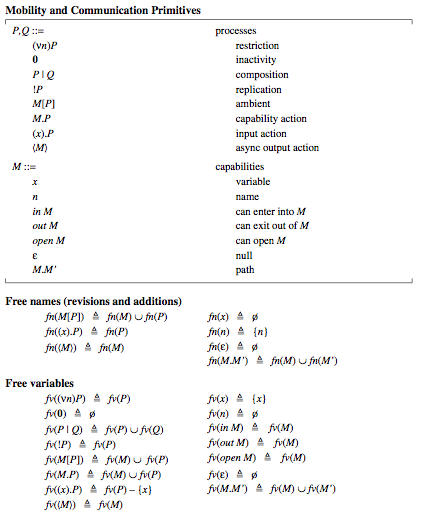
\includegraphics[scale=1]{ambient.png}
  \end{center}
  \captionsetup{justification=centering}  
  \caption{Syntax and scope in the ambient-calculus \\ -- \citep{Cardelli98mobileambients}}
  \label{ambient-syn}
\end{table}

\begin{table} [p]
  \begin{center}
  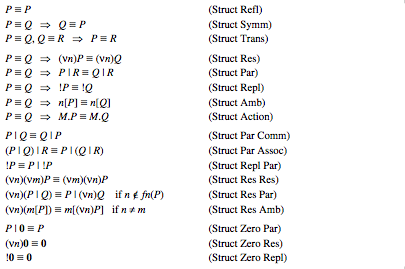
\includegraphics[scale=1]{ambient_str_1.png}
  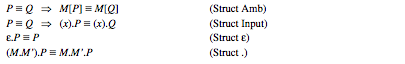
\includegraphics[scale=1]{ambient_str_2.png}
  \end{center}
  \captionsetup{justification=centering}    
  \caption{Structure congurence in the ambient-calculus \\ -- \citep{Cardelli98mobileambients}}
  \label{ambient-str}
\end{table}

\begin{table} [p]
  \begin{center}
  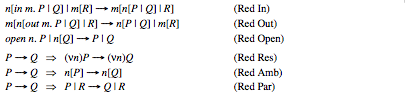
\includegraphics[scale=1]{ambient_red_1.png}
  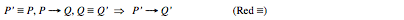
\includegraphics[scale=1]{ambient_red_2.png}
  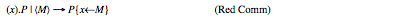
\includegraphics[scale=1]{ambient_red_3.png}
  \end{center}
  \captionsetup{justification=centering}    
  \caption{Reduction in the ambient-calculus \\ -- \citep{Cardelli98mobileambients}}
  \label{ambient-red}
\end{table}

\subsubsection{The Obliq Programming Language}
At the time of writing this report, there is no real language that implements the ambient-calculus\footnote{\citet{VMAmbient} proposed a virtual machine for the ambient calculus.}.  Instead,  this section will introduce the Obliq language, which has certain notions of ambient and influenced the design of the ambient calculus.

Obliq\citep{obliq} is one of the earliest programming languages which support distributed programming.  The language was designed before the pervasive of web applications.  It only supports simple object model which is a collection of fields.  Each field of an Obliq object could be a value (a constant or a procedure), a method, or an alias to an object.  An object could either be constructed directly by specifying its fields, or be cloned from other objects.  

The four operations which could be performed on objects are:
\begin{itemize}
  \item selection: a value field of a object could be selected and transmitted over the web.  If the selected value is a constant, the value will be transmitted.  By contrast, if the selected value is a method, values of its arguments will be transmitted to the remote site where the method is defined, the computation is performed remotely, and the result or an exception is returned to the site of the selection.
  \item updating: when an updating operation is performed on an remote object, the selected filed is updated to a value that might be sent across the web.  If the selected filed is a method, a transmission of method closure is required.
  \item cloning: cloning an object will yield a new object which contains all fields of argument objects or raise an error if field names of argument objects conflict.
  \item aliasing:  After executing an aliasing method, a.x := $\bf{alias}$ y $\bf{of}$ b $\bf{end}$, further operations on x of a will be redirected to y of b.
\end{itemize}

It is important to note that Obliq, as some other languages in the pre-web era, does not distinguish local values from distributed values.  By contrast, \citet{dis_note} pointed out that distinct views must be adopted for local and distributed objects, due to differences in latency, memory access, partial failure, and concurrency.
% \subsection{Type-parameterized Actor libraries}



% \subsection{Reliability Studies}

\section{Summing Up}

To review, the Actor Model \citep{Hewitt:1973} is proposed for designing 
concurrent systems. It is employed by Erlang  \citep{ArmstrongErlang} and other 
programming languages. Erlang developers designed the Supervision Principle in 
1998 when the Erlang/OTP library was released as an open-source project.  With 
the supervision principle, actors are supervised by their supervisors, who are 
responsible for initializing and monitoring their children.  Erlang developers 
claimed that applications using the supervision principle have achieved a 
high availability \citep{ArmstrongAXD}. Recently, the actor programming model 
and the supervision principle have been ported to Akka, an Actor library 
written in Scala.  Although Scala is a statically typed language and provides a 
sophisticated type system, the type of messages sent to Akka actors are 
dynamically checked when they are processed.  The next chapter presents the 
design and implementation of the TAkka library where type checks are involved
at the earliest opportunity to expose type errors.





 \chapter{TAkka: Design and Implementation}
\label{takka_design}

\begin{center}
(This chapter is expanded from the companion paper, Chapter 3 and 4)
\end{center}
\vspace{12 pt}

Last Chapter examined actor programming and supervision in Erlang/OTP and Akka. 
 Erlang/OTP is written in Erlang, a dynamically typed language, whereas Akka is 
written in Scala, a statically typed language. A key advantage of static typing 
is that it detects some type errors at an early stage, i.e., at compile time.  
Nevertheless, messages sent to Akka actors are dynamically typed. 

\begin{comment}
because it was believed that 
type parameterized actors and supervision will be difficult
to work together [? private communication and mailing list question ?] .
\end{comment}

This Chapter presents the design of the TAkka library, which confirms the key 
claim of this thesis: actors in supervision trees can be 
{\it statically} typed by parameterizing the actor class with the type of 
messages it expects to receive.  The Chapter outlines how 
static and dynamic type checking are used to prevent ill-typed messages.  
Examples of TAkka applications show that type-parameterized actors can form 
supervision trees in the same way as actors without type parameters.  This 
Chapter concludes with a brief discussion on design alternatives used by 
other actor libraries.

The latest TAkka library is built on top of Akka 2.1.4.  During the research 
of this project, TAkka has been built on stable Akka releases since 2.0.  For 
all Akka versions, actors can be parameterized as expected.  
Nevertheless, as the Akka API and the structure of Akka configuration file change 
slightly in different Akka versions, readers who want to use a later Akka 
version may need to update the API or the configuration file according to the 
specification of the Akka version used.


\section{TAkka Example: a String Counter}
\label{sec:takka_example}

The introduction of TAkka begins with an illustrative TAkka example in Figure~\ref{takka_string_counter}. The example is ported from the string counter 
example given in Figure~\ref{fig:akka_string_counter}.  The TAkka code is 
similar to its Akka equivalent, with a few differences marked in 
\textcolor{blue}{blue}.  

First, the {\tt Actor} class in TAkka takes a type 
parameter which indicates the type of expected messages.  In our example, {\tt 
StringCounter} is an actor which only expects String messages.  Consequently, 
its {\tt typedReceive} function has a function type {\tt String => Unit}.  The 
type is not explicitly declared in code because it can be inferred and checked 
by the Scala type system.  In an Eclipse IDE with Scala plug-in, the following 
type information is shown on the screen when the {\tt typedReceive} 
method is mouseovered:
\begin{lstlisting}[language=scala]
  def typedReceive: String => Unit
\end{lstlisting}%
The type of {\tt m} at line 8, which is {\tt String}, is omitted too because it can be 
inferred as well.

Second, the type of messages sending to an actor reference is statically 
checked. In the TAkka version of the {\tt StringCounterTest}, the Scala 
language infers that the  type of {\tt counter}, declared at line 16, has type 
{\tt ActorRef[String]}.  This means that only String messages can be sent to {\tt 
counter}.   Sending a non-String message (i.e. line 21) results in a compile error.

Third, dynamic type checking is involved at the earliest opportunity when 
static type checking meets its limitation.  For example, when a user looks up 
an actor reference by its type and path, as at line 23 and 26, 
TAkka does not statically check if there will be an actor of a 
compatible type at that path when the program is executed.  Although the type 
error at line 26 is not statically detected, an exception is expected to raise
as soon as the ill-typed actor reference is claimed at run time (line 26), 
earlier than the time when the actor reference is used (line 29).  
The terminal output shows that the print statement
at line 28 has not been executed when the exception is raised.  The result confirms that
the exception is raised by code at line 26.



\begin{figure}
      \begin{lstlisting}[language=scala, escapechar=?]
package sample.takka

import ?\textcolor{blue}{takka}?.actor.{Actor, ActorRef, ActorSystem, Props}

class StringCounter extends ?\textcolor{blue}{Actor[String]}? {
  var counter = 0;
  def ?\textcolor{blue}{typedReceive}? = {
    case m => 
      counter = counter +1
      println("received "+counter+" message(s):\n"+m)
  }
}

object StringCounterTest extends App {
  val system = ActorSystem("StringCounterTest")
  val counter = system.actorOf(Props[?\textcolor{blue}{String}?, StringCounter], 
"counter")
  
  counter ! "Hello World"
//  counter ! 1
// type mismatch; found : Int(1) required: String  
  val counterString = 
system.actorFor?\textcolor{blue}{[String]}
?("akka://StringCounterTest/user/counter")
  counterString ! "Hello World Again"
  val counterInt = 
system.actorFor?\textcolor{blue}{[Int]}
?("akka://StringCounterTest/user/counter")  
// dynamic type error!  
  println("Hello")  // will not be executed
  counterInt ! 2      // will not be executed
}

/*
Terminal Output:

received 1 message(s):
	Hello World
received 2 message(s):
	Hello World Again
Exception in thread "main" java.lang.Exception: 
ActorRef[akka://StringCounterTest/user/counter] does not exist
or does not have type ActorRef[Int]
 */	
    \end{lstlisting}
    \caption{TAkka Example: A String Counter}
    \label{takka_string_counter}
\end{figure}


Because sending an actor a message of unexpected type is prevented,
there is no need to define a handler for unexpected messages in our TAkka
example.  Eliminating ill-typed messages benefits both users and developers
of actor-based services. For users, since messages are transmitted 
asynchronously, it is easier to trace the source of potential errors if they are 
captured earlier, especially in a distributed environment. For service 
developers, they can focus on the logic of the services rather than worrying 
about incoming messages of unexpected types.


\section{Type-parameterized Actor}
\label{takka_actor}
A TAkka actor has type {\tt Actor[M]}.  It inherits the Akka {\tt Actor} 
trait to minimize implementation effort.  Users of the TAkka library, 
however, do not need to use any Akka Actor API.  Instead, programmers are 
encouraged to use the typed interface given in Figure~\ref{takka_actor_api}.  
Unlike other actor libraries, every TAkka actor class takes a type parameter 
{\tt M} which specifies the type of messages expected by the actor.  The same 
type parameter is used as the input type of the {\tt typedReceive} function.  
The actor reference pointing to itself, {\tt typedSelf}, has type {\tt 
ActorRef[M]} to which only messages of type {\tt M} can be sent.  
Finally, the actor context for the actor, {\tt typedContext}, has type {\tt ActorContext[M]}.  

To maintain the actor behaviour and the supervision relationship, a special class
of messages, which has type {\tt SystemMessage}, should be handled by all actors.
Unlike the Akka design, which handles system messages in the {\tt receive} block,
system messages are handled in a separate method, namely the {\tt systemMessageHandler} method.
System messages and its handler will be discussed in detail at Section~\ref{systemmessage}.


\begin{figure}[h]
\begin{lstlisting}[language=scala, escapechar=?]
package takka.actor

abstract class ?\textcolor{blue}{Actor[M:Manifest]}? extends akka.actor.Actor
  protected def ?\textcolor{blue}{typedReceive}?:?\textcolor{blue}{Function}?[?\textcolor{blue}{M}?, Unit]
  
  val ?\textcolor{blue}{typedSelf}?:ActorRef?\textcolor{blue}{[M]}?
  val ?\textcolor{blue}{typedContext}?:ActorContext?\textcolor{blue}{[M]}?
  var supervisorStrategy: SupervisorStrategy
  ?\textcolor{blue}{def systemMessageHandler:SystemMessage => Unit}?
  
  def preStart(): Unit
  def preRestart(reason: Throwable, message: Option[Any]): Unit
  def postRestart(reason: Throwable): Unit
  def postStop(): Unit
\end{lstlisting}
\caption{TAkka API: Actor}
\label{takka_actor_api}
\end{figure}

Notice that the type of {\tt typedReceive} is {\tt Function[M, Unit]}, whereas 
the type of {\tt receive} in the Akka {\tt Actor} class is {\tt 
PartialFunction[Any, Unit]}.  An 
advantage of using {\tt Function} is that the compiler can check the 
completeness of the domain patterns.  In Akka, completeness checking is not considered
because an Akka actor may receive messages of any type.  In contrast, a TAkka 
actor only expects messages of a certain type.  Therefore, pattern completeness 
checking is a helpful feature for TAkka users.

The two immutable fields of {\tt Actor}, {\tt typedContext} and 
{\tt typedSelf}, are automatically initialized when the actor is created.
Library users may override the default supervisor strategy in the
way explained in Section~\ref{supervision}.  The implementation of the {\tt
typedReceive} method, on the other hand, is always provided by users.

Types of variables and methods that do not related to message passing are not
type parameterized (i.e. {\tt supervisorStrategy}, {\tt preStart}, {\tt postRestart}, and {\tt postStop}).
The {\tt preRestart} method has the same type as the Akka version.  It is invoked before the
actor is restarted due to an error (i.e. {\tt reason}) that {\it might be} caused when processing a message (i.e. {\tt message}).
Because an actor can be evolve to a version that handles more types of messages (Section~\ref{hot_swapping}),
the type of the problematic message cannot be determined in advance.  It is fine to
define some message patterns that will never be triggered at run-time.


Notice that {\tt takka.actor.Actor} inherits {\tt akka.actor.Actor}.  A 
critical problem of using inheritance is that dynamically typed 
Akka API, which we are trying to avoid whenever possible, are still available 
to TAkka users.  Unfortunately, this limitation cannot be overcome by using 
delegation because, as we have seen in Akka API, a child actor is created by 
calling the {\tt actorOf} method from its supervisor's actor context, which 
cannot be accessed outside the supervisor. {\tt Actor} is the only TAkka 
class that is implemented using inheritance. All other TAkka classes and traits 
are either implemented by delegating tasks to Akka counterparts or rewritten in 
TAkka.  To overcome the limitation, a complete reimplementation of that TAkka
Actor library is required.  The author estimates that the required work is
similar to implementing the Akka Actor library.


\section{Type-parameterized Actor Reference}
\label{takka_actor_ref}

The last section explains the type-parameterised Actor class, {\tt  
Actor[M]}, whose message handler only considers messages of the expected 
type {\tt M}.  Such a design only works in a system which either provides a 
reasonable handler for undefined messages at the receiver side,  or is able to 
prevent ill-typed messages at the sender side.  As mentioned in Section 
\ref{message mailbox}, undefined messages are handled differently in Erlang and 
different Akka versions.  Each mechanism has its own rationale.  
Unfortunately, there is no known single mechanism that meets the requirements of 
all applications.  The Akka development team tends to provide more ways to 
handle unexpected messages at the receiver side.  In contrast,  the TAkka 
library is aimed at preventing ill-typed messages at the sender side.  
We achieve this goal by adding a type parameter to the {\tt ActorRef} class.

The API of {\tt ActorRef} is given in Figure~\ref{takka_actor_reference_api}.  
The {\tt ActorRef} class takes two parameters: one type 
parameter that indicates the type of expected message and one implicit 
argument that records the {\tt Manifest} of the type parameter.  In most 
cases, the implicit {\tt Manifest} can be provided by the Scala language 
automatically.


\begin{figure}[h]
\begin{lstlisting}[language=scala,  escapechar=?]
package takka.actor 

abstract class ActorRef?{\textcolor{blue}{[-M](implicit mt:Manifest[M])}?
  ?{\textcolor{blue}{val untypedRef:akka.actor.ActorRef}? 

  def !(message: ?{\textcolor{blue}{M}?):Unit
  ?{\textcolor{blue}{def publishAs[SubM<:M](implicit smt:Manifest[SubM]):ActorRef[SubM]}?

  abstract def path: akka.actor.ActorPath
  final def compareTo(other: ActorRef?{\textcolor{blue}{[\_]}?): Int
  final def equals(that: Any): Boolean
  // no forward method

\end{lstlisting}
\caption{TAkka API: Actor Reference}
\label{takka_actor_reference_api}
\end{figure}

As in Erlang and Akka, users send a message to an actor via the {\tt !} 
method of its actor reference.   Sending an actor a message of a different type 
causes an error at compile time.  By using type-parameterized actor references, 
the receiver does not need to worry about unexpected messages, while senders 
can be sure that messages will be understood and processed, as long as the 
message is delivered.







\begin{figure}[p]
\begin{lstlisting}[language=scala,  escapechar=?]
package sample.takka

import takka.actor.ActorRef
import takka.actor.ActorSystem
import takka.actor.Props
import takka.actor.Actor

sealed trait Operation
case class Multiplication(m:Int, n:Int) extends Operation
case class Division(m:Int, n:Int) extends Operation

class Calculator extends Actor?{\textcolor{blue}{[Operation]}? {
  def ?{\textcolor{blue}{typedReceive}? = {
    case Multiplication(m:Int, n:Int) =>
      println(m +" * "+ n +" = "+ (m*n))    
    case Division(m, n) =>
      println(m +" / "+ n +" = "+ (m/n))
  }
}

object TAkkaActorRefTest extends App{
  val system = ActorSystem("MySystem")
  val calculator:ActorRef[Operation] = system.actorOf(Props[?{\textcolor{blue}{Operation}?, Calculator], "calculator")
  
  // explicit type conversion 
  ?{\textcolor{blue}{val multiple = calculator.publishAs[Multiplication]}?

  // implicit type conversion 
  val divide:ActorRef[Division] = calculator  
  
  calculator ! Multiplication(3, 2)
  multiple ! Multiplication(3, 3)
  //  multiple ! Division(6, 2)  
  //Compiler Error: type mismatch; found : sample.takka.Division
  //	  required: sample.takka.Multiplication
  divide ! Division(6, 2)  
}

/*
Terminal Output:
3 * 2 = 6
3 * 3 = 9
6 / 2 = 3
*/
\end{lstlisting}
\caption{TAkka Example: Typed Actor Reference}
\label{takka_actor_reference_example}
\end{figure}


An actor can usually react to a finite set of different message patterns, 
whereas our notation of actor reference only takes one type parameter.  In a 
type system that supports untagged union types, no special extension is
required.  In a type system which supports polymorphism, {\tt ActorRef} should
be contravariant on its type argument {\tt M}, denoted as {\tt ActorRef[-M]} in 
Scala.  To understand why {\tt ActorRef} is contravariant, let us consider both the 
{\it Get and Put Principle} and an illustrative example.   {\tt ActorRef} is 
contravariant because users only {\tt put} values to an actor reference (using the {\tt !} method) but 
never get values out of it.  Fetching the value sent via an actor reference is done
in the {\tt typedReceive} method of the {\tt Actor} class.  The illustrative example considered here is a 
simple calculator defined in Figure~\ref{takka_actor_reference_example}.
The calculator defined in the example can compute the result of two types of 
operations: multiplication and division.  Hence, {\tt Division} is a 
subtype of {\tt Operation}. It is clear that {\tt ActorRef[Operation]} is a 
subtype of {\tt ActorRef[Division]} because if users can send both 
multiplication requests and division requests to an actor reference, they can 
send division requests only to that actor reference.

For ease of use, {\tt ActorRef} provides a {\tt publishAs} method that 
casts an actor reference to a version that only accepts a subset of supported 
messages.  The {\tt publishAs} method encapsulates the process of type cast on 
{\tt ActorRef}, a contravariant type.  The author believes that using the 
notation of the {\tt publishAs} method can be more intuitive than thinking 
about contravariance 
and subtyping relationship each time, especially when publishing an actor 
reference as different types in a complex application.  In addition, type 
conversion using {\tt publishAs} is statically type checked.  More importantly, 
with the {\tt publishAs} method, users can give a supertype of an actor 
reference on demand, without defining new supertypes and modify affected 
classes in the type hierarchy, some of which may not be accessible by application developers.

\section{Type Parameterized Props}
\label{takka_actor_porps}
An instance of type {\tt Props[M]} is used when creating an actor of type {\tt 
Actor[M]}.  A Prop of type {\tt Prop[M]} can be created by one of 
the two factory methods provided by the {\tt Props} object.

\begin{figure}[!h]
\begin{lstlisting}[language=scala, escapechar=?]
package takka.actor

final case class Props?\textcolor{blue}{[-T](props: akka.actor.Props)}?

object Props
  def apply?\textcolor{blue}{[T, A<:Actor[T]] (implicit arg0: 
Manifest[A])}?: Props[T] 
  def apply?\textcolor{blue}{[T](clazz: Class[\_ <: Actor[T]], 
args:Any*)}: Props[T]
\end{lstlisting}
    \caption{TAkka API: Props}
    \label{takka_props}
\end{figure}

In Figure~\ref{takka_string_counter}, a Props for creating an instance of {\tt 
StringCounter} is created by the following code
\begin{lstlisting}[language=scala]
  Props[String, StringCounter]
\end{lstlisting}
In the above code, Scala checks that {\tt StringCounter} is a 
subtype of\\ {\tt Actor[String]}, and provides a value for the implicit 
parameter, which has type {\tt Manifest[StringCounter]}.

The TAkka {\tt Props} class is contravariant on its type parameter because 
users can create an actor by providing a {\tt Props} instance that is able to 
create actors that can handle more types of messages.


\section{Type Parameterized Actor Context}
\label{takka_actor_context}

An actor context describes the contextual information of an actor. Because each 
actor is an independent computational primitive, an actor context is private to 
its corresponding actor.  By using API in Figure 
\ref{takka_api_actor_context}, an actor can
\begin{enumerate}[(\itshape i\upshape)]
\item create a child actor supervised by itself,
\item fetch some of its states,
\item retrieve an actor reference 
corresponding to a given actor path and type using the {\tt actorFor} method,
\item set a timeout denoting the time within which
a new message must be received using the {\tt setReceiveTimeout} method, and
\item update its behaviours using the {\tt become} method.  
\end{enumerate}

Compared with corresponding Akka API, TAkka methods take an additional type 
parameter: {\tt M}, {\tt SupM}, or {\tt Msg}.  The type variable {\tt M} is
the same as the type parameter of the {\tt ActorContext} class, which corresponds
to the type parameter of the {\tt Actor} class.  The later in turn is the same
as the input type of its {\tt typedReceive} method.  Therefore, the {\tt props}
method has type {\tt Props[M]} because it is used to create an actor of type {\tt Actor[M]}.
The {\tt typedSelf} value has type {\tt ActorRef[M]} because it records the 
actor reference to its corresponding actor.  The {\tt SupM} type variable in the
{\tt become} method performs a static check for backward compatible behaviour
upgrade, a topic elaborated in Section~\ref{hot_swapping}.  
The {\tt Msg} type variable in {\tt actorOf}, {\tt remoteActorOf}, and {\tt actorFor}
denotes the type parameter of another actor.  Therefore, {\tt Msg} has no
relationship with the other two type variables.



\begin{figure}[p]
      \begin{lstlisting}[language=scala, escapechar=?]
package takka.actor

abstract class ActorContext?\textcolor{blue}{[M:Manifest]}?
  def actorOf ?\textcolor{blue}{[Msg]}? (props: ?\textcolor{blue}{Props[Msg]}?)
                       ?\textcolor{blue}{(implicit mt:  Manifest[Msg])}?: ActorRef[Msg]
  def actorOf ?\textcolor{blue}{[Msg]}? (props: ?\textcolor{blue}{Props[Msg]}?, name: String)
                       ?\textcolor{blue}{(implicit mt: Manifest[Msg])}?: ActorRef[Msg]

  @throws(classOf[NotRemoteSystemException])
  ?\textcolor{blue}{  def remoteActorOf[Msg](props:Props[Msg])}?
                       ?\textcolor{blue}{(implicit mt:Manifest[Msg]):ActorRef[Msg]}?
  @throws(classOf[NotRemoteSystemException])
  ?\textcolor{blue}{  def remoteActorOf[Msg](props:Props[Msg], name:String)}?
                       ?\textcolor{blue}{(implicit mt:Manifest[Msg]) :ActorRef[Msg]}?

  // no child, children, and parent
  
  def props:Props?\textcolor{blue}{[M]}?
  lazy val typedSelf:ActorRef?\textcolor{blue}{[M]}?
  // no sender

  implicit def system : ActorSystem 
  
  def actorFor?\textcolor{blue}{[Msg]}? (actorPath: String)
       ?\textcolor{blue}{(implicit mt: Manifest[Msg]): ActorRef[Msg]}?
  def actorFor?\textcolor{blue}{[Msg]}?(actorPath: 
    akka.actor.ActorPath)?\textcolor{blue}{(implicit mt:Manifest[Msg]): 
ActorRef[Msg]}?

  // no watch, unwatch, and stop    

?\textcolor{blue}{  def become[SupM >: M]( }?
      ?\textcolor{blue}{newTypedReceive: SupM => Unit, }?
      ?\textcolor{blue}{newSystemMessageHandler: }?
      ?\textcolor{blue}{SystemMessage => Unit, }?
      ?\textcolor{blue}{newpossiblyHarmfulHandler:akka.actor.PossiblyHarmful => Unit }?
      ?\textcolor{blue}{)(implicit smt:Manifest[SupM]):ActorRef[SupM]  }?
  
  // no unbecome

  def setReceiveTimeout (timeout: Duration): Unit  
  def receiveTimeout : Duration

    \end{lstlisting}
    \caption{TAkka API: Actor Context}
    \label{takka_api_actor_context}
\end{figure}

An actor creates a child actor using the {\tt actorOf} method or the {\tt 
remoteActorOf} method.  If no user-specified name is provided for the child, a 
system-generated one will be used.  The {\tt actorOf} method returns a TAkka 
actor reference which internally maintains a type descriptor and an Akka actor 
reference.  Notice that, the Akka actor reference returned by the Akka system 
cannot be used remotely because its actor path does not include an IP address 
and a port number.  The {\tt remoteActorOf} method is implemented in TAkka as a 
complement to {\tt actorOf}.  The {\tt remoteActorOf} returns an actor 
reference that can be used remotely if the actor system enables remote 
communication, otherwise it raises a {\tt NotRemoteSystemException}.  Calling 
{\tt remoteActorOf} takes longer than calling {\tt actorOf} because the IP 
address and port number need to be fetched from the system configuration.
The way to enable distributed programming will be explained in Section 
\ref{sec_distributed_calculator}.


The contextual information of an actor includes the {\tt Props} used to create 
that actor, the typed actor reference pointing to that actor, and the actor 
system where the actor resides.  TAkka removes API that enquire the 
actor reference of an actor's parent and children for two reasons.  Firstly, 
the types of the parent and children of an actor are unknown to the library 
developer as they vary from one actor to another.  Secondly, actor references 
to parent and children of an actor can be obtained using the {\tt actorFor} 
method if their paths and types are known by the user.  A TAkka actor context 
does not record the value of the {\tt sender} because its type changes for each 
message.  The author recommends the Erlang-style message pattern, in which the 
actor reference to the message sender is part of the message if the sender 
expects a reply message.

The two {\tt actorFor} methods are used for fetching an actor reference of the 
expected type located at an actor path.  The task of type checking and 
reference fetching is
delegated to the actor system (Section~\ref{sec:takka_look_up_actor_reference}),
which implements the same API.

The method signature of the {\tt setReceiveTimeout} method and the \\
{\tt receiveTimeout} method are the same as the Akka version.  The
{\tt setReceiveTimeout} method sets a timeout within which a 
new message is expected to be received.  The {\tt receiveTimeout} method returns
the set timeout.  In Akka, if no message is received within the specified 
timeout, a {\tt ReceiveTimeout} {\it message} is sent to the actor itself.  
In Akka, the {\tt ReceiveTimeout} message and other messages are handled by the 
{\tt receive} method.  In TAkka, the {\tt ReceiveTimeout} message is 
handled by the {\tt systemMessageHandler} method separately.  Section 
\ref{systemmessage} explains the TAkka design in depth.

Finally, TAkka defines the {\tt become} method with a new signature so that 
behaviour upgrade is backward compatible.  To guarantee backward 
compatibility, the {\tt unbecome} method is removed.  The next 
section explains behaviour upgrade in TAkka.



\section{Backward Compatible Behaviour Upgrade}
\label{hot_swapping}

The {\tt become} method enables behaviour upgrade of an 
actor.  The {\tt become} method in TAkka is different from behaviour 
upgrades in  Akka in two aspects.  Firstly, as the handler for system messages 
is separated from the handler for other messages, TAkka users may update the 
system message handler as well.  Secondly, behaviour upgrade in TAkka {\it must} be 
backward compatible and {\it cannot} be rolled back.  In other words, an actor 
must evolve to a version that is at least capable of handling all messages accepted
by the previous version.  The above decision was made so that a service published to 
users will not be unavailable later.  


\begin{figure}[p]
\begin{lstlisting}
package takka.actor

abstract class ActorContext[M:Manifest] {
  implicit private var mt:Manifest[M] = manifest[M]

  def become[SupM >: M](
      behavior: SupM => Unit
  )(implicit smtTag:Manifest[SupM]):ActorRef[SupM] ={
    become(behavior, this.systemMessageHandler, this.possiblyHarmfulHandler)   
  }
  
  def become[SupM >: M](
      behavior: SupM => Unit, 
      newSystemMessageHandler:SystemMessage=>Unit
  )(implicit smtTag:Manifest[SupM]):ActorRef[SupM] = {
    become(behavior, newSystemMessageHandler,  this.possiblyHarmfulHandler)   
  } 
  
  def become[SupM >: M](
      newTypedReceive: SupM => Unit,
      newSystemMessageHandler:
               SystemMessage => Unit
      newpossiblyHarmfulHandler:akka.actor.PossiblyHarmful => Unit
  )(implicit smtTag:Manifest[SupM]):ActorRef[SupM] = {
     val smt = manifest[SupM]
     if (!(smt >:> mt))
       throw BehaviorUpdateException(smt, mt)

    this.mt = smt
    this.systemMessageHandler =  newSystemMessageHandler
    this.possiblyHarmfulHandler = newpossiblyHarmfulHandler
    
    new ActorRef[SupM] {
      val untypedRef = untypedContext.self
    }
  }
}

case class BehaviorUpdateException(smt:Manifest[_], mt:Manifest[_]) extends Exception(smt + "must be a supertype of "+mt+".")
\end{lstlisting}
\caption{Behaviour Upgrade in TAkka}
\label{takka_become}
\end{figure}

The {\tt become} method is implemented as shown in Figure~\ref{takka_become}.  
The design of the {\tt become} method involves both static type checking 
and dynamic type checking.  The static type parameter {\tt M} should be 
interpreted as the least general type of messages expected by an actor 
of type {\tt Actor[M]}, whose initial message handler has a function type {\tt M=>Unit}.
When a user decides to upgrade the message handler of an actor, it is
important to make sure that the new message handler is aware of all
types of messages that may be sent to an actor before the
upgrade.  Backward compatible behaviour upgrade requires that the input type of a 
new message handler should be a supertype of the input type of the old message 
handler.  Unfortunately, the concrete type of the new message handler will only 
be known when the {\tt become} method is invoked. When a series of {\tt become} 
invocations are made at run time, the order of those invocations may be 
non-deterministic.  Therefore, it is not possible to guarantee backward 
compatibility by using static type checking only.
As a result, dynamic type checking is required.  To do so, each {\tt 
TypedContext} instance records the manifest of the input 
type of the current message handler.  The recorded manifest is used to check if 
the input type of the new message handler is a {\it supertype} of the 
input type of the current message handler.  If so, both the manifest and the 
message handler are updated.  Although static type checking meets its 
limitation, it prevents some invalid {\tt become} invocations at compile time.

\begin{figure}[p]
\begin{lstlisting}[language=scala, escapechar=?]
package sample.?\textcolor{blue}{takka}?
import takka.actor.{ActorRef, ActorSystem, Props, Actor}

?\textcolor{blue}{trait Operation}?
?\textcolor{blue}{trait BasicOperation extends Operation}?
case class Multiplication(m:Int, n:Int) ?\textcolor{blue}{extends BasicOperation}?
case class Upgrade?\textcolor{blue}{[Op >: BasicOperation]}?(advancedCalculator:?\textcolor{blue}{Op=>Unit}?)
                                               ?\textcolor{blue}{extends BasicOperation }?
class CalculatorServer extends Actor?\textcolor{blue}{[BasicOperation]}? { 
  def ?\textcolor{blue}{typedReceive}? = {
    case Multiplication(m:Int, n:Int) => 
      println(m +" * "+ n +" = "+ (m*n))
    case Upgrade(advancedCalculator) =>
      println("Upgrading ...")
      ?\textcolor{blue}{typedContext}?.become(advancedCalculator)    
  }
}
object CalculatorUpgrade extends App {
  val system = ActorSystem("CalculatorSystem") 
  val simpleCal:ActorRef[BasicOperation] = system.actorOf(Props[?\textcolor{blue}{BasicOperation}?, CalculatorServer], "calculator")
  simpleCal ! Multiplication(5, 1)
  
  case class Division(m:Int, n:Int) extends Operation
  def advancedCalculator:Operation=>Unit = {
    case Multiplication(m:Int, n:Int) => 
      println(m +" * "+ n +" = "+ (m*n))
    case Division(m:Int, n:Int) => 
      println(m +" / "+ n +" = "+ (m/n))
    case Upgrade(_) =>
      println("Upgraded.")
  }
  simpleCal ! Upgrade(advancedCalculator)    
  val advancedCal = system.actorFor?\textcolor{blue}{[Operation]}?("akka://CalculatorSystem/user/calculator")   
  advancedCal ! Multiplication(5, 3)
  advancedCal ! Division(10, 3)
  advancedCal ! Upgrade(advancedCalculator)
}
/*  Terminal Output:
5 * 1 = 5
Upgrading ...
5 * 3 = 15
10 / 3 = 3
Upgraded.
 */
\end{lstlisting}
  \caption{TAkka Example: Backward Compatible Behaviour Upgrade}
  \label{fig:takka_swap} 
\end{figure}

The code in Figure~\ref{fig:takka_swap} demonstrates how to upgrade the message 
handler in TAkka.  The code is similar to the Akka example in Figure 
\ref{fig:akka_swap}.  The calculator server begins with a basic version, which
can only compute multiplication but leaves the developer an 
opportunity to upgrade it later.   The {\tt CalculatorUpgrade} test simulates a 
simple scenario.  After using the basic calculator server for a while, the 
service developer implements an advanced message handler, {\tt 
advancedCalculator}, which supports both multiplication and division.  The 
developer updates the server by sending an {\tt Upgrade} message that contains 
the new message handler.  When the upgrade has been completed, users can 
send {\tt Division} messages to the server.

There are two differences between the TAkka version (Figure 
\ref{fig:takka_swap}) and the Akka version (Figure~\ref{fig:akka_swap}).  First, two 
new types, namely {\tt Operation} and {\tt BasicOperation}, are introduced. The {\tt 
BasicOperation} trait is defined to be used as the type parameter of the {\tt 
CalculatorServer} class.  The {\tt Operation} trait is not required for the 
basic calculator.  The {\tt Operation} trait is provided so that the developer 
can define new types of operation in addition to those basic ones.  Second, 
there is no {\tt Downgrade} message in the TAkka version.  A user who has an 
actor reference of type {\tt ActorRef[Operation]} must always ensure that a division 
request can be understood by the server.



\section{Typed Name Server}
\label{nameserver}

In distributed systems, a name server maps each registered name, usually a
unique string, to a dynamically typed value, and provides a function to look up 
a value for a given name. A name can be encoded as a {\tt Symbol} in Scala so 
that names which represent the same string have the same value.  As a value 
retrieved from a name server is {\it dynamically typed}, it needs to be checked 
against and be cast to an expected type at the client side before using it.

To overcome the limitations of the untyped name server, TAkka provides
a typed name server which maps each registered typed name to a value of the
corresponding type, and allows look up of a value by giving a typed name.  Our 
typed name server can be straightforwardly ported to other platforms that 
support type reflection.

\begin{figure}[p]
\begin{lstlisting}[language=scala]
package takka.nameserver

import scala.collection.mutable.HashMap
import scala.reflect.Manifest
import scala.Symbol

case class TSymbol[-T:Manifest](val s:Symbol) {
    private [takka] val t:Manifest[_] = manifest[T]
    override def hashCode():Int = s.hashCode()  
}

case class TValue[T:Manifest](val value:T){
  private [takka] val t:Manifest[_] = manifest[T]
}

object NameServer {
  private val nameMap = new HashMap[TSymbol[_], TValue[_]]

  def set[T:Manifest](name:TSymbol[T], value:T):Boolean = synchronized {
    val tValue = TValue[T](value)
    if (nameMap.contains(name)){ return false }
    else{
      nameMap.+=((name, tValue))
      return true
    }
  }

  def unset[T](name:TSymbol[T]):Boolean = synchronized {
    if (nameMap.contains(name)  && nameMap(name).t <:< name.t  ){
      nameMap -= name
      return true
    }else{ return false }
  }  

  def get[T](name:TSymbol[T]):Option[T] = synchronized {
    if (!nameMap.contains(name)) {return None}
    else { 
      val tValue = nameMap(name)
      if (tValue.t <:< name.t) { return Some(tValue.value.asInstanceOf[T]) }
      else{ return None }
    }
  }
}
\end{lstlisting}
  \caption{Typed Name Server}
  \label{fig:takka_nameserver} 
\end{figure}




\subsection{Typed Name and Typed Value}

A typed name, {\tt TSymbol}, is a name shipped with a type descriptor.  A 
typed value, {\tt TValue}, is a value shipped with a type descriptor, which
describes a supertype of the most precise type of that value.  
In Scala, {\tt TSymbol} and {\tt TValue} can be simply defined as in Figure
\ref{fig:takka_nameserver}.

In the Scala implementation, {\tt TSymbol} is declared as a {\it case class} so that it can be 
used as a data constructor and for pattern matching.  In addition, the
type descriptor, {\tt t}, is constructed automatically and is private to the
{\tt takka} package so that only the library developer can access it as a field 
 of {\tt TSymbol}. {\tt TValue} is declared as a {\it case class} for the same 
reason.  The {\tt hashCode} method of {\tt TSymbol} does not consider the
value of its type descriptor for efficiency considerations.

\subsection{Operations}

With the notion of {\tt TSymbol}, a typed name server provides 
the following three operations:
\begin{itemize}
  \item {\tt set[T:Manifest](name:TSymbol[T], value:T):Boolean}

The {\tt set} operation registers a typed name with a value of corresponding 
type and returns true if the symbolic representation of {\it name} has {\it 
not} been registered; otherwise the typed name server discards the request and
returns false.


  \item {\tt unset[T](name:TSymbol[T]):Boolean}

The {\tt unset} operation removes the entry {\it name} and returns true if (i) 
its symbolic representation is registered and (ii) the type {\tt T} is a 
supertype of the registered type; otherwise the operation returns false.

  \item {\tt get[T](name:TSymbol[T]):Option[T]}

The {\tt get} operation returns Some(v:{\tt T}), where {\tt v} is the value 
associated with {\it name}, if (i) {\it name} is a registered name and (ii) 
{\tt T} is a supertype of the registered type; otherwise the operation returns 
None.
\end{itemize}

The TAkka library implements the typed name server using the code given in 
Figure~\ref{fig:takka_nameserver}.  The typed name server internally saves and 
fetches data by using a standard hashmap data structure.  The API are designed 
with the following considerations.  

Firstly, when an operation fails, the name server returns {\tt false} or {\tt 
None} rather than raising an exception.  The decision is made so that the name 
server is always available.  Keeping a name server alive is important 
especially if the name server permits distributed enquiries, in which case the 
remote caller would like to have feedback.  Although it seems that the 
current name server is only available to applications running in the same JVM, 
as Section~\ref{sec:takka_look_up_actor_reference} will explain, distributed 
enquiries can be easily supported via another application that supports 
distributed communication, for example, by using a TAkka actor.

Secondly, the {\tt unset} method and the {\tt get} method succeed as long as the 
associated type of the input name is a supertype of the associated type of the 
registered name.  In other words, a user must know how the value is registered. 
For the {\tt get} method, the returned value shall be used as a supertype of 
the registered type, which may have fewer methods. To permit polymorphism while 
keeping the efficiency of using hashmap, the {\tt hashCode} method of {\tt 
TSymbol} does not take its type manifest into account.  Equivalence comparison 
on {\tt TSymbol} instances, however, considers the type.  The {\tt hashCode} 
method of {\tt TSymbol} ignores its type description so that it has an 
additional benefit.  As typed symbols that have the same symbolic representation 
have the same hash value, the design prevents the situation where users 
accidentally register 
two typed names with the same symbolic representation but different types, 
in which case if one type is a supertype of the other, the return value of {\tt 
get} may be non-deterministic.  In our design, only names that have not been 
registered can be added to the name server.  Therefore, the {\tt set} method 
does not need to check the type information as in the {\tt unset} method and 
the {\tt get} method.  Because the type information in {\tt TSymbol} is ignored 
in the hashmap, it is recorded in the notion of {\tt TValue}, which 
does not appear in the API for library users.  

Lastly, the implementations of the three operations are thread safe.  They are 
{\tt synchronized} to prevent thread interference and memory consistency errors.
When one thread is executing one of the methods of {\tt NameServer}, all other 
threads that invoke its methods are suspended. The {\tt nameMap} is a private 
field to {\tt NameServer} so that other objects cannot directly access it.  
Finally, the three simple operations are executed without interactions with 
other objects.  Therefore, there is no liveness issue for the implementation.

\subsection{Dynamic Type Comparison}

In general, dynamic type checking can be carried out in two ways.  The first 
method is to check whether the most precise type of a value conforms to the
structure of a data type.  Examples of this method include dynamically typed
languages and the {\tt instanceOf} method in Java and other languages.  The
second method is to compare two type descriptors at run time.  The
implementation of our typed name server uses the second method because  
it detects type errors which may otherwise be left out in the first method.  Our
implementation requires the runtime type reification feature provided by Scala.
In a system that does not support type reification, implementing typed name 
servers is more difficult.


%\newpage
\section{Look up Typed Actor References via Actor System}
\label{sec:takka_look_up_actor_reference}

The same as in as in Akka, a TAkka actor system organises related actors in a tree 
structure and provides services such as thread scheduling, network connection, 
and logging.  The API of the TAkka {\tt ActorSystem} class is given in Figure 
\ref{takka_api_actor_system}.  Because the functionality of a TAkka actor system 
is almost the same as an Akka {\tt ActorSystem}, the TAkka {\tt ActorSystem} is 
implemented by managing an Akka {\tt ActorSystem} as its private field, to 
which dynamically typed tasks are delegated.   % In addition to using the Akka 
% library functions, a TAkka {\tt ActorSystem} employs both static and dynamic 
% type checking to detect type errors.  This section explains how the typed 
% name server, described in the last section, is used when creating and fetching type 
% parameterized actor references.

In addition to delegating some tasks to an Akka actor system, a TAkka actor 
system uses the typed name server (Section~\ref{nameserver}) in the same JVM to save typed actor 
references created by that actor system.  Each TAkka actor system initializes 
an {\tt ActorTypeChecker} instance that is responsible for enquiring whether a 
typed actor reference is registered at the typed name server located at the JVM 
it runs.  In this section, Figure~\ref{takka_actorOf} presents the code of the 
{\tt actorOf} function which creates an actor and registers its actor reference 
to the typed name server.  Figure~\ref{takka_actorFor} presents the code of the 
{\tt actorFor} function which fetches typed actor references.


\begin{figure}[h]
\begin{lstlisting}[language=scala, escapechar=?]
package takka.actor

case class NotRemoteSystemException(system:ActorSystem) extends Exception("ActorSystem: "+system+" does not support remoting")

object ActorSystem
    def apply():ActorSystem 
    def apply(sysname: String): ActorSystem 
    def apply(sysname: String, config: Config): ActorSystem 
    def apply(sysname: String, config: Config, 
               classLoader: ClassLoader): ActorSystem

abstract class ActorSystem
    private val system:akka.actor.ActorSystem
    def stop(actorRef:ActorRef?\textcolor{blue}{[\_]}?)
    def deadLetters : ActorRef?\textcolor{blue}{[Any]}?
    def isTerminated: Boolean
    
    def actorOf?\textcolor{blue}{[Msg:Manifest]}?(props:Props?\textcolor{blue}{[Msg]}?):ActorRef?\textcolor{blue}{[Msg]}?
    def actorOf?\textcolor{blue}{[Msg:Manifest]}?(props:Props?\textcolor{blue}{[Msg]}?, 
                                  name:String):ActorRef?\textcolor{blue}{[Msg]}?
    
    @throws(classOf[NotRemoteSystemException])
    def remoteActorOf?\textcolor{blue}{[Msg:Manifest]}?(props:Props?\textcolor{blue}{[Msg]}?):ActorRef?\textcolor{blue}{[Msg]}?
    @throws(classOf[NotRemoteSystemException])
    def remoteActorOf?\textcolor{blue}{[Msg:Manifest]}?(props:Props?\textcolor{blue}{[Msg]}?, 
                                          name:String):ActorRef?\textcolor{blue}{[Msg]}?
        
    def actorFor?\textcolor{blue}{[M:Manifest]}?(actorPath: String): ActorRef?\textcolor{blue}{[M]}?
    def actorFor?\textcolor{blue}{[M:Manifest]}?(actorPath: akka.actor.ActorPath): ActorRef?\textcolor{blue}{[M]}?
\end{lstlisting}
    \caption{TAkka API: Actor System}
    \label{takka_api_actor_system}
\end{figure}




\begin{figure}[p]
\begin{lstlisting}[language=scala]
object ActorSystem {
  def apply(sysname: String, config: Config,
             classLoader: ClassLoader): ActorSystem = 
    new ActorSystem {
      val system = akka.actor.ActorSystem(sysname, config, classLoader)
      system.actorOf(akka.actor.Props(new ActorTypeChecker),
                       "ActorTypeChecker")
    }
}
abstract class ActorSystem {
  private val system:akka.actor.ActorSystem  
  @throws(classOf[NotRemoteSystemException])
  def host:String
  def actorOf[Msg:Manifest](props:Props[Msg],
                                 name:String):ActorRef[Msg] = {
    val actor = new ActorRef[Msg] {
      val untypedRef = system.actorOf(props.props, name) }
    NameServer.set(TSymbol[ActorRef[Msg]](Symbol(actor.path.toString())), 
                     actor)
    actor
  }  
  @throws(classOf[NotRemoteSystemException])
  def remoteActorOf[Msg:Manifest](props:Props[Msg], 
                                          name:String):ActorRef[Msg] = {
    val akkaactor = actorOf[Msg](props:Props[Msg], aname:String)
    val actor = new ActorRef[Msg] {
      val localPathStr = akkaactor.path.toString()
      val takka_system = this
      val sys_path = localPathStr.split("@")
      val remotePathStr = sys_path(0)+"@"+takka_system.host+":"+takka_system.port+sys_path(1)
      //e.g. akka://RemoteCreation@129.215.91.195:2554/user/...
      val untypedRef = system.system.actorFor(remotePathStr)
    }
    NameServer.set(TSymbol[ActorRef[Msg]](scala.Symbol(actor.path.toString())), 
                     actor)
    actor
  }

  private class ActorTypeChecker extends akka.actor.Actor{
    def receive = {
      case Check(path, t) =>
        NameServer.get(TSymbol(Symbol(path.toString))(t) ) match {
          case None => sender ! NonCompatible
          case Some(_) => sender ! Compatible
  } }}
}
\end{lstlisting}
    \caption{Actor System: actorOf}
    \label{takka_actorOf}    
\end{figure}


\begin{figure}[p]

\begin{lstlisting}[language=scala]
def actorFor[M:Manifest](actorPath: akka.actor.ActorPath): ActorRef[M]= {
    val isRemotePath = actorPath.address.host match {
      case None => false
      case Some(_) => true
    }
    
    if (isRemotePath) {
      val untyped_ref:akka.actor.ActorRef = system.actorFor(actorPath)      
      //e.g. "akka://CalculatorApplication@127.0.0.1:2552/user/ActorTypeServer"
      val remoteChecker:akka.actor.ActorRef  = 
      system.actorFor("akka://"+actorPath.address.system+"@"
                                   +actorPath.address.host.get+":"
                                   +actorPath.address.port.get+"/user/ActorTypeServer")
      implicit val timeout = new akka.util.Timeout(10000) // 10 seconds
      val checkResult = remoteChecker ? Check(actorPath, manifest[M]) 
      var result:ActorRef[M] = null
      checkResult onSuccess {
        case Compatible => 
          result = new ActorRef[M]{
            val untypedRef = untyped_ref
          } 
        case NonCompatible => 
          throw new Exception("ActorRef["+actorPath+"] does not exist 
                  or does not have type ActorRef["+manifest[M]+"]")
      }
      result
    }else{
      // local actor reference, fetch from local name server
      NameServer.get(TSymbol[ActorRef[M]](scala.Symbol(actorPath.toString))) 
      match {
        case None => 
          throw new Exception("ActorRef["+actorPath+"] does not exist 
                   or does not have type ActorRef["+manifest[M]+"]")
        case Some(ref) => 
          new ActorRef[M]{
        	  val untypedRef = system.actorFor(actorPath)
          }
      }
    }
  }
\end{lstlisting}
    \caption{Actor System:  actorFor}
    \label{takka_actorFor}
\end{figure}


The {\tt actorOf} method and the {\tt remoteActorOf} method create an actor 
that is supervised by a {\tt user} actor created by the system.  The task of 
creating an actor is delegated to an Akka actor system, which is a private field 
of a TAkka actor system.  The additional work done by the TAkka actor system is 
to register the typed actor path and the typed actor reference into the typed 
name server running in the same JVM (line 17 and line 33 in Figure 
\ref{takka_actorOf} ).  Because an actor reference returned by the Akka  
{\tt actorOf} method cannot be used remotely as it does not contain an IP 
address and a port number, the TAkka library defines a {\tt remoteActorOf} 
method which returns a typed actor reference that contains information 
required for using it remotely.  If remote communication is not enabled by the 
actor system, a {\tt NotRemoteSystemException} will arise.


The {\tt actorFor} method returns a typed actor reference if there is such with 
an expected type located at a given path.  When looking for a typed 
actor reference, the actor system first checks if the input actor path 
contains an IP address and a port number.  If so, it sends a request to the 
{\tt ActorTypeServer} actor in the remote actor system; otherwise it sends a 
request to the {\tt ActorTypeServer} actor in the local machine.  When an {\tt 
ActorTypeServer} actor receives a request that asks if there is an actor 
reference of the expected type at a given path,
it checks registered names at the typed name server in its JVM.  


Although a typed name server defined in the current TAkka implementation can 
only be directly called by applications running on the same JVM.  As the 
implementation of {\tt actorFor} shows, it can indirectly receive remote 
requests via applications that support distributed communication, for example, 
TAkka actors.  The design of a consistent global shared typed name server is 
left as a future extension.



\section{Supervisor Strategies}
\label{supervision}

The TAkka library uses the Akka supervisor strategies explained in Section 
\ref{akka_supervision}: {\tt OneForOne} and {\tt AllForOne}.  If a supervisor 
adopts the {\tt OneForOne} strategy, it restarts its child when it fails.  
The failure of an actor will not affect its siblings.  If a supervisor adopts 
the {\tt AllForOne} supervisor strategy, all children will 
be restarted when any of them fails.  The third OTP supervisor strategy, {\tt
RestForOne}, restarts children in a user-specified order, and hence is not
supported by Akka as it does not specify an order of initialization for
children.  The {\tt RestForOne} supervisor strategy can be simulated by 
grouping related children and defines special messages to trigger actor 
terminations.  The TAkka library does not implement the {\tt RestForOne} 
strategy because it is not needed for the applications considered in this 
project.

Figure~\ref{takka_supervisor_strategy} gives API of supervisor strategies in 
TAkka.  In fact, it is the same as the Akka version given in Figure 
\ref{akka_supervisor_strategy}.  TAkka reuses the Akka API because none of the 
supervisor strategies requires type-parameters and TAkka separates 
the message handler for system messages and the message handler for other 
messages.




\begin{figure}[h]
    \begin{lstlisting}    
package akka.actor
abstract class SupervisorStrategy
case class OneForOne(restart:Int, time:Duration)(decider: Throwable => 
  Directive) extends SupervisorStrategy
case class OneForAll(restart:Int, time:Duration)(decider: Throwable => 
  Directive) extends SupervisorStrategy

sealed trait Directive extends AnyRef
object Escalate extends Directive
object Restart extends Directive
object Resume extends Directive
object Stop extends Directive
    \end{lstlisting}
    \caption{TAkka API: Supervisor Strategies}
    \label{takka_supervisor_strategy}
\end{figure}






\begin{comment}
As shown in the API, an Akka supervisor strategy can choose different 
reactions for different reasons of child failures in its {\tt decider} 
parameter.  Recall that {\tt Throwable} is the superclass of {\tt Error} and 
{\tt Exception} in Scala and Java.  Therefore, users can pattern match on 
possible types and values of {\tt Throwable} in the {\tt decider} function.  In 
other words, when the failure of a child is passed to the {\tt decider} 
function of the supervisor, it is matched to a pattern that reacts to that 
failure.

The {\tt decider} function contains user-specified computations and returns a 
value of {\tt Directive} that denotes the standard recovery process implemented 
by the Akka library developers.  The {\tt Directive} trait is an enumerated 
type that has four possible values: the
{\tt Escalate} action which throws the exception to the supervisor of the 
supervisor, the {\tt Restart} action which replaces the failed child with a new 
one, the {\tt Resume} action which asks the child to process the message again, 
and the {\tt Stop} action which terminates the failed actor permanently.


As in OTP, for each supervisor strategy, users can specify the maximum number of
restarts of any child within a period.  The default supervisor strategy in 
TAkka is {\tt OneForOne} that permits unlimited restarts.  {\tt Directive} is 
an enumerated type with the following values: the {\tt Escalate} action which 
throws the exception to the supervisor of the supervisor, the {\tt Restart} 
action which replaces the failed child with a new one, the {\tt Resume} action 
which asks the child to process the message again, and the {\tt Stop} action 
which terminates the failed actor permanently.

\end{comment}

A TAkka Safe Calculator example is given in Figure 
\ref{takka_safe_calculator} as a reminder of the Akka Safe Calculator in 
Figure~\ref{akka_supervised_calculator}. Both examples define a simple 
calculator which supports multiplication and division. The simple calculator 
does not consider the problematic case of dividing a number by 0, in which case 
an {\tt ArithmeticException} will raise. A fault tolerant calculator, safe 
calculator, is defined as the supervisor of the simple calculator. The safe 
calculator delegates calculation tasks to the simple calculator and restarts 
it when an {\tt ArithmeticException} raises. The supervisor 
strategy of the safe calculator also specifies the maximum failures its child 
may have within a time range. If the child fails more frequently than the 
allowed frequency, the safe calculator will be stopped, and its failure will be 
reported to its supervisor, the system guardian actor in this example.  The 
terminal output shows that the simple calculator is restarted before the next 
message is delivered.

The TAkka implementation is modified from the Akka version with changes marked 
in \textcolor{blue}{blue}.  First, an {\tt Operation} trait is introduced as 
the supertype of the {\tt Multiplication} message and the {\tt Division} 
message.  Second, actor classes are parameterized by the type of messages they 
expected.  Third, the {\tt calculator} actor reference in TAkka can publish 
itself as an actor reference, {\tt multiplicator}, which only accepts 
multiplication requests. The supervisor strategy used in the TAkka 
implementation is exactly the same as the one in the Akka implementation.

\begin{figure}[p]
    \begin{lstlisting}[language=scala, escapechar=?]
package sample.takka
import takka.actor.{ActorRef, ActorSystem, Props, Actor}
?\textcolor{blue}{sealed trait Operation}?
case class Multiplication(m:Int, n:Int) ?\textcolor{blue}{extends Operation}?
case class Division(m:Int, n:Int) ?\textcolor{blue}{extends Operation}?
class Calculator extends ?\textcolor{blue}{Actor[Operation]}? {
  def ?\textcolor{blue}{typedReceive}? = {
    case Multiplication(m:Int, n:Int) =>
      println(m +" * "+ n +" = "+ (m*n))    
    case Division(m, n) =>
      println(m +" / "+ n +" = "+ (m/n))
  }
}
class SafeCalculator extends ?\textcolor{blue}{Actor[Operation]}? {
  import language.postfixOps
  override val supervisorStrategy =
    OneForOneStrategy(maxNrOfRetries = 2, withinTimeRange = 1 minute) {
      case _: ArithmeticException  =>
        println("ArithmeticException Raised to: "+self)
        Restart
    }
  val child:ActorRef[Operation] = 
         typedContext.actorOf(Props[Operation, Calculator], "child")
  def ?\textcolor{blue}{typedReceive}? = {    case m => child ! m  }
}
object SupervisorTest extends App{
  val system = ActorSystem("MySystem")
  val calculator:?\textcolor{blue}{ActorRef[Operation]}? = 
        system.actorOf(?\textcolor{blue}{Props[Operation, Calculator]}?, "calculator")
  ?\textcolor{blue}{val multiplicator = calculator.publishAs[Multiplication]}?
  
  calculator ! Multiplication(3, 2)
  multiplicator ! Multiplication(3, 3)
//  multiplicator ! Division(6, 2)  
//  Compiler Error: type mismatch; found : sample.takka.Division 
//  required: 	 sample.takka.Multiplication
  calculator ! Division(10, 0)
  calculator ! Division(10, 5)
}  
/*  Terminal Output:
3 * 2 = 6
3 * 3 = 9
java.lang.ArithmeticException: / by zero
ArithmeticException Raised to: Actor[akka://MySystem/user/safecalculator]
10 / 5 = 2
*/
    \end{lstlisting}
    \caption{TAkka Example: Supervised Calculator}
    \label{takka_safe_calculator}
\end{figure}

\newpage

\section{Handling System Messages}
\label{systemmessage}

Actors communicate with each other by sending messages.  To organize actors, a 
special category of messages should be handled by all actors.  In Akka, those 
messages are subclasses of the {\tt PossiblyHarmful} trait.  The TAkka library 
defines messages of the same name as subclasses of the {\tt SystemMessage} trait.


\begin{table}[h]
\begin{center}
\begin{tabular}{| l | c | c | c | c |}
  \hline
  Message & TAkka 2.0 & TAkka 2.1 & Akka 2.0 & Akka 2.1 \\
  \hline
  Kill  & public & public & public & public \\
  \hline
  PoisonPill & public & public & public & public \\
  \hline
  ReceiveTimeout & public & public & public & public \\
  \hline
  ChildTerminated & public & private & public & private \\
  \hline
  Restart & public & private & public & private \\
  \hline
  Terminated & not included & not included & public & public \\
  \hline
  Create  & private & private & public & private \\
  \hline
  Failed  & private & private & public & private \\
  \hline
  Link  & not included & not included & public & private \\
  \hline  
  Unlink  & not included & not included & public & private \\
  \hline 
  Suspend  & private & private & public & private \\
  \hline
  Resume  & private & private & public & private \\
  \hline
\end{tabular}
\end{center}
\caption{System Messages}
\label{system_messages}
\end{table}

Table~\ref{system_messages} lists system messages used in Akka and TAkka.
Some messages are defined as public objects which can be handled by a user where
as some messages are defined as private objects which only be used by the
library developers.  TAkka retains {\tt Kill} and {\tt PoisonPill} because it is used
in the Chaos Monkey library and the Supervision View 
library explained in Section~\ref{reliability}.  TAkka users may want to use those two messages for
reliability test as well.  The {\tt ReceiveTimeout} message is retained because it is used in many 
applications considered in this thesis.  The TAkka library makes {\tt Create}, {\tt Failed}, {\tt Suspend}, 
and {\tt Resume} private because reactions to those messages can be consistently defined
in library rather than leave to users.  The decision is verified by the design
of Akka 2.1, which makes all above messages private as well.  Akka 2.1 also makes
{\tt ChildTerminated} and {\tt Restart} private for the same reason.  The author
does not recognise this point in the design of TAkka 2.0 and follow the Akka design
in TAkka 2.1.  The TAkka library does not retain {\tt Terminated}, {\tt Link}, and {\tt Unlink} because, as will be explained in 
Section~\ref{alternative_designs}, life-cycle monitor relationship outside the 
supervision tree is considered as a redundant design.

The purpose of those messages are examples as the followings.

\paragraph{Kill}   An actor that receives this message will send an {\tt ActorKilledException} 
to its supervisor.

\paragraph{PoisonPill}  An actor that receives this message will be permanently terminated.  The
supervisor cannot restart the killed actor.

\paragraph{ReceiveTimeout}  A message sent from an actor to itself when it has not received a message
after a timeout.

\paragraph{ChildTerminated(child: ActorRef[M])}  A message sent from a child actor to its supervisor before it terminates.
  
\paragraph{Restart}A message sent from a supervisor to its terminated child asking the
child to restart.

\paragraph{Terminated}  When an actor monitors the life cycle of another actor using Akka Death 
Watch \citep[Section 3.1]{akka_doc}, the watcher will receive a 
Terminated(watched) message when the {\it watched} actor is terminated.

\paragraph{Create} A message sent to the created actor itself.
  
\paragraph{Failed}  An actor sends itself a {\tt Failed(cause: Throwable)} message when an error 
of {\tt cause} occurs when it is processing messages.
  
\paragraph{Link} A message sent to linked actors when Akka Death Watch \citep[Section 
3.1]{akka_doc} is used.

\paragraph{Unlink}  A message sent to linked actors when Akka Death Watch \citep[Section 
3.1]{akka_doc} is disabled. 

\paragraph{Suspend}   A message sent by the system to an actor asking it suspend the process of 
processing remaining messages in its mailbox.

\paragraph{Resume}  A message sent by the system to an actor to dissolve the effects of the {\tt 
Suspend} message so that the actor will resume the process of processing 
messages in its mailbox.





The next question is whether a system message should be handled by the library 
or by application developers.  In Erlang and early versions of Akka, all
system messages can be explicitly handled by developers in the {\tt receive}
block.  In recent Akka versions, some system messages become private to library 
developers and some can be still handled by application developers.

As there are only two kinds of supervisor strategies to
consider, both of which have clearly defined operational behaviours, all
messages related to the liveness of actors are handled in the TAkka library. 
Application developers may indirectly affect the system message handler via 
specifying
the supervisor strategies. In contrast, messages related to the behaviour of an
actor, e.g. {\tt ReceiveTimeout}, are better handled by application
developers. In TAkka, {\tt ReceiveTimeout} is the only system message that can
be explicitly handled by users.  Nevertheless, the {\tt SystemMessage}
trait is defined in the library so that new system messages can be included in 
the future when required.

A key design decision in TAkka is to separate handlers for the system messages 
and user-defined messages.  The above decision has two benefits. Firstly,
the type parameter of actor-related classes only need to denote
the type of user defined messages rather than the untagged union of user 
defined messages and the system messages.  Therefore, the TAkka design applies
to systems that do not support untagged union type.  Secondly, since 
system messages can be handled by the default handler, which applies
to most applications, users can focus on the logic of handling user
defined messages.







\section{Case Study: A Distributed Calculator}
\label{sec_distributed_calculator}

In previous sections, we have seen that an actor can be parameterized by the 
type of messages it expects.  Adding type parameters to actors does not affect 
the construction of supervision trees because system messages are separated 
from other messages.  Because the TAkka library delegates the tasks of actor 
creation and message sending to the underlying Akka system, distributed 
communication can be done in TAkka in the same way as in Akka.  

The example used in this section is modified from the example in \citep[Section 
5.11]{akka_doc}.  In this example, two calculators will be created as actors, 
one basic calculator that can compute addition and subtraction, one 
advanced calculator that can compute multiplication and division.  The basic 
calculator will be created locally as previous examples.  The advanced 
calculator will be created at a remote machine by updating the actor system 
configuration.  Actor references for local and remote actors are retrieved in 
the same way.


\subsection{Actor System Configuration for Distribution}

Application developers can override the default configuration of an Akka actor 
system by providing an alternative {\tt Config} object or load the 
configuration from an {\tt application.conf} file in the application deployment 
folder. \citep{akka_doc}  The configuration of a TAkka actor system is 
modified by changing the {\tt Config} object which is used by the underlying 
Akka actor system.  The details of Akka system configuration are explained in 
the Akka documentation.  This section only explains the configuration used in 
the distributed calculator example.  For details of Akka actor system 
configuration, readers are directed to look at the Akka documentation for the 
version they are using.

The configuration in Figure~\ref{discal_distribute_configuration} is used 
for the {\tt RemoteCreation} system in Figure~\ref{discal_distribute_creation}. 
The configuration overrides three system policies.  Firstly, the system enables 
distributed communication by replacing the actor reference provider from 
{\tt LocalActorRefProvider} to {\tt RemoteActorRefProvider}.  Secondly, the 
{\tt deployment} block specifies that actor created at the logical path  
{\tt /advancedCalculator} shall be physically created by the {\tt 
CalculatorApplication} actor system located at address {\tt 
129.215.91.88:2552}.  Finally, the actor system itself is located at address
{\tt 129.215.91.195:2554}.   In this example, {\tt 129.215.91.88} and {\tt 
129.215.91.195} are two IP addresses allocated for the Ethernet connection at 
the author's office.  {\tt 2552} and {\tt 2554} are port numbers that are not 
used by the two computers used for this test.


\begin{figure}[h]
\begin{lstlisting}
akka{
  actor {
    provider = "akka.remote.RemoteActorRefProvider"
    deployment {
       /advancedCalculator {
         remote = "akka://CalculatorApplication@129.215.91.88:2552"
    }}}
    remote {
       netty {
         hostname = "129.215.91.195"
         port = 2554               
    }
  }
}
\end{lstlisting}
\caption{Configuration Example: Distributed Creation}
\label{discal_distribute_configuration}
\end{figure}

% \newpage
\subsection{A Complete Example}

The classes defined for the example described at the beginning of this section 
are the followings:


\begin{figure}[p]
\begin{lstlisting}
package typed.remote.calculator
import takka.actor.{Actor, ActorRef}
import akka.actor.ActorPath
import scala.reflect.runtime.universe._

trait MathOp
case class Add(nbr1: Int, nbr2: Int) extends MathOp
case class Subtract(nbr1: Int, nbr2: Int) extends MathOp
case class Multiply(nbr1: Int, nbr2: Int) extends MathOp
case class Divide(nbr1: Double, nbr2: Int) extends MathOp

trait CalculatorMessage
case class Op(op:MathOp, sender:ActorRef[MathResult])                    
     extends CalculatorMessage
     
trait MathResult
case class AddResult(nbr: Int, nbr2: Int, result: Int)                   
     extends MathResult
case class SubtractResult(nbr1: Int, nbr2: Int, result: Int)                    
     extends MathResult
case class MultiplicationResult(nbr1: Int, nbr2: Int, result: Int)       
     extends MathResult
case class DivisionResult(nbr1: Double, nbr2: Int, result: Double)       
     extends MathResult
case class Ask(calculator:ActorRef[CalculatorMessage], op:MathOp) 
     extends MathResult
     


class AdvancedCalculatorActor extends Actor[CalculatorMessage] {
  def typedReceive = {
    case Op(Multiply(n1, n2), sender) =>
      println("Calculating %d * %d".format(n1, n2))
      sender ! MultiplicationResult(n1, n2, n1 * n2)
    case Op(Divide(n1, n2), sender) =>
      println("Calculating %.0f / %d".format(n1, n2))
      sender ! DivisionResult(n1, n2, n1 / n2)
  }
}
\end{lstlisting}
\caption{Distributed Calculator: Messages and Advanced Calculator}
\label{discal_message}
\end{figure}

\begin{figure}[p]
\begin{lstlisting}
package typed.remote.calculator
import akka.kernel.Bootable
import takka.actor.{ Props, Actor, ActorSystem }
import com.typesafe.config.ConfigFactory

class SimpleCalculatorActor extends Actor[CalculatorMessage] {
  def typedReceive = {
    case Op(Add(n1, n2), sender) =>
      println("Calculating %d + %d".format(n1, n2))
      sender ! AddResult(n1, n2, n1 + n2)
    case Op(Subtract(n1, n2), sender) =>
      println("Calculating %d - %d".format(n1, n2))
      sender ! SubtractResult(n1, n2, n1 - n2)
  }
}
class CalculatorApplication extends Bootable {
  val system = ActorSystem("CalculatorApplication",
               ConfigFactory.parseString(""" 
                 akka{
                   actor {
                     provider = "akka.remote.RemoteActorRefProvider"
                   }
                   remote {
                     netty {                       
                       hostname = "129.215.91.88"
                       port = 2552       
                     }
                   }
                 }""") )
  val cal = system.actorOf(Props[CalculatorMessage, 
                            SimpleCalculatorActor], "simpleCalculator")
}

object CalcApp {
  def main(args: Array[String]) {
    new CalculatorApplication
    println("Started Calculator Application - waiting for messages")
  }
}
\end{lstlisting}
\caption{Distributed Calculator: Simple Calculator Local Creation}
\label{discal_local_creation}
\end{figure}

\begin{figure}[p]
\begin{lstlisting}
package typed.remote.calculator
import akka.kernel.Bootable
import com.typesafe.config.ConfigFactory
import scala.util.Random
import takka.actor._

class CreationApplication extends Bootable {
  val system = ActorSystem("RemoteCreation", 
                           ConfigFactory.parseString(""" 
                 akka{
                   actor {
                     provider = "akka.remote.RemoteActorRefProvider"
                     deployment {
                       /advancedCalculator {
                         remote = 
                                "akka://CalculatorApplication@129.215.91.88:2552"
                   }}}
                   remote {
                     netty {
                       hostname = "129.215.91.195"
                       port = 2554               
                 }}}""") )
  val localActor = system.actorOf(Props[MathResult, CreationActor],
                                                    "creationActor")
  val remoteActor = system.actorOf(Props[CalculatorMessage, 
                          AdvancedCalculatorActor], "advancedCalculator")

  def doSomething(op: MathOp) = {    localActor ! Ask(remoteActor, op)  }
}
class CreationActor extends Actor[MathResult] {
  def typedReceive = {
    case Ask(calculator, op) => {
      calculator ! Op(op, typedRemoteSelf)      
    }
    case result: MathResult => result match {
      case MultiplicationResult(n1, n2, r) => 
        println("Mul result: %d * %d = %d".format(n1, n2, r))
      case DivisionResult(n1, n2, r)  => 
        println("Div result: %.0f / %d = %.2f".format(n1, n2, r))
}}}

object CreationApp extends App {
    val app = new CreationApplication
    while (true) {
      if (Random.nextInt(100) % 2 == 0) 
         app.doSomething(Multiply(Random.nextInt(20), 
                                      Random.nextInt(20)))
      else app.doSomething(Divide(Random.nextInt(10000),
                                      (Random.nextInt(99) + 1)))
      Thread.sleep(200)
}}

\end{lstlisting}
\caption{Distributed Calculator: Distributed Creation}
\label{discal_distribute_creation}
\end{figure}

\begin{figure}[p]
\begin{lstlisting}
package typed.remote.calculator
import akka.kernel.Bootable
import scala.util.Random
import com.typesafe.config.ConfigFactory
import takka.actor.{ ActorRef, Props, Actor, ActorSystem }

class LookupApplication extends Bootable {
  val system = ActorSystem("LookupApplication", 
                           ConfigFactory.parseString(""" 
                 akka{
                   actor {
                     provider = "akka.remote.RemoteActorRefProvider"
                   }

                   remote {
                     netty {
                       hostname = "129.215.91.195"
                       port = 2553               
                     }
                   }
                 }""") )
  val actor = system.actorOf(Props[MathResult, LookupActor], "lookupActor")
  val remoteActor = system.actorFor[CalculatorMessage]
       ("akka://CalculatorApplication@129.215.91.88:2552/user/simpleCalculator")

  def doSomething(op: MathOp) = {    actor ! Ask(remoteActor, op)  }
}
class LookupActor extends Actor[MathResult] {
  def typedReceive = {
    case Ask(calculator, op) => {      calculator ! Op(op, typedRemoteSelf)    }
    case result: MathResult => result match {
      case AddResult(n1, n2, r)      => 
           println("Add result: %d + %d = %d".format(n1, n2, r))
      case SubtractResult(n1, n2, r) => 
           println("Sub result: %d - %d = %d".format(n1, n2, r))
    }
  }
}
object LookupApp extends App {
    val app = new LookupApplication
    while (true) {
      if (Random.nextInt(100) % 2 == 0) 
         app.doSomething(Add(Random.nextInt(100), Random.nextInt(100)))
      else 
           app.doSomething(Subtract(Random.nextInt(100), 
                                        Random.nextInt(100)))
      Thread.sleep(200)
    }
}
\end{lstlisting}
\caption{Distributed Calculator: Actor Look up}
\label{discal_lookup}
\end{figure}

\paragraph{Operations and Messages} The Operations ({\tt MathOp}) considered in 
this example are addition ({\tt Add}), subtraction ({\tt Subtract}), 
multiplication ({\tt Multiply}), and division ({\tt Divide}).  There are two 
types of messages used in this example: the {\tt CalculatorMessage} sent to a 
real calculator that can computes an operation; the {\tt MathResult} sent to a 
broker who receives calculation requests and display the result of each 
calculation.


\paragraph{Calculators} The two calculator actors defined in this example are 
the \\ {\tt SimpleCalculatorActor} in Figure~\ref{discal_local_creation} and 
the {\tt AdvancedCalculatorActor} in Figure~\ref{discal_message}.  The simple 
calculator can compute addition and subtraction while the advanced calculator 
can compute multiplication and division.


\paragraph{Test Applications} There are three test applications in this example.
The {\tt CalApp} application creates an actor system with name {\tt 
CalculatorApplication} located at address {\tt 129.215.91.88:2552}.  Inside the 
actor system, a simple calculator is created.  The {\tt CreationApp} 
application creates two actors: one {\tt CreationActor} at the local machine 
and one {\tt AdvancedCalculatorActor} at a remote node.  The {\tt 
CreationActor} is used as a broker that sends a request to the advanced 
calculator and print the returned result.  Finally, the {\tt LookupApp} 
application works as the same as the {\tt CreationApp} except that the remote 
actor used in this application is the simple calculator fetched from the 
{\tt actorFor} method.

\vspace{12 pt}

The example code shows that distributed programming is TAkka is enabled in the 
same way as in Akka, that is, by updating the actor system configuration.  For 
an Akka application that enables distributed programming, the same actor system 
configuration can be reused in the corresponding TAkka version.


\newpage

\section{Design Alternatives}
\label{alternative_designs}

\paragraph{Akka Typed Actor}
In the Akka library, there is a special class called {\tt TypedActor}, which
contains can be supervised by an actor.  The {\tt TypedActor} class is essentially
a different framework.  A service of {\tt TypedActor} class is invoked by method 
invocation instead of message passing.  Code in Figure~\ref{akka typed actor} shows 
how to define a simple string processor using Akka typed actor.  
Line 34 to 36 show that a {\tt TypedActor} object does not have a {\tt !} method.
Line 37 to 39 and their output (Line 44 to 45) show that an actor is located at 
the given address but messages sent to that actor using its actor reference are
unhandled.

The Akka {\tt TypedActor} class prevents some type errors but have two limitations. Firstly, {\tt TypedActor} does not 
permit behaviour upgrade.  Secondly, avoiding the type pollution 
problem, explained in Section~\ref{type_pollution}, by 
using Akka typed actors is the same inconvenience as using a simple object-oriented 
model, where supertypes need to be defined in advance.  In Scala and Java, 
introducing a supertype in a type hierarchy requires modification to all 
affected classes, whose source code may not be accessible by application 
developers.


\begin{figure}[p]

\begin{lstlisting}
package sample.akka;

import akka.actor.ActorSystem
import akka.actor.Props
import akka.actor.TypedActor
import akka.actor.TypedProps
import akka.actor.UnhandledMessage

trait StringCounterTypedActor{
  def processString(m:String) 
}

class StringCounterTypedActorImpl (val name:String) extends 
StringCounterTypedActor{
  private var counter = 0;
  def this() = this("default")
  
  def processString(m:String) {
    counter = counter +1
    println("received "+counter+" message(s):\n\t"+m)
  }
}

object StringCounterTypedActorTest extends App {
  val system = ActorSystem("StringCounterTest")
  val counter:StringCounterTypedActor = 
TypedActor(system).typedActorOf(TypedProps[StringCounterTypedActorImpl](), 
"counter")
  counter.processString("Hello World")
  
  val handler = system.actorOf(Props(new MessageHandler()))
  system.eventStream.subscribe(handler,classOf[akka.actor.UnhandledMessage]);
  
//  counter ! "Hello World"  
//  Compiler Error:  
//   value ! is not a member of sample.akka.StringCounterTypedActor
  val counterRef = system.actorFor("akka://StringCounterTest/user/counter")
  counterRef ! "Hello World Again"
  counterRef ! 2
}
/*  Terminal Output:
received 1 message(s):
	Hello World
unhandled message:Hello World Again
unhandled message:2
 */		
\end{lstlisting}
\caption{Akka Example: String Counter using Akka TypedActor}
\label{akka typed actor}
\end{figure}



\paragraph{Actors with or without Internal Mutable States}
The actor model formalized by \citet{Hewitt:1973} does not 
specify its implementation strategy.  In Erlang, a functional programming 
language, actors do not have mutable states.  It is recommended that the state 
of an actor, if there is any, to be saved in an {\it ETS} table, a data structure 
provided by the OTP library \citep{ErlangManual}.  In Scala, users are free
to use mutable variables in code.
The TAkka library is built on top of Akka and implemented in Scala.  
As a result, TAkka does not prevent users from defining actors with 
mutable states.  
Nevertheless, the author of this thesis encourages the use of 
actors in a functional style, for example encoding the {\tt sender} of a 
synchronous message as part of the incoming message rather than a state 
of an actor, because it is difficult to synchronize mutable
states of replicated actors in a cluster environment.

In a cluster, resources are replicated at different locations to provide 
fault-tolerant services.  The CAP theorem \citep{CAP} states that it is
impossible to achieve consistency, availability, and partition tolerance in a
distributed system simultaneously.  For actors that use mutable state, system 
providers have to either sacrifice 
availability or partition tolerance, or modify the consistency model.  For 
example, Akka actors have mutable state and Akka cluster developers
expand a great deal of effort to implement an eventual consistency model \citep{Kuhn12}.
In contrast, stateless services, e.g. RESTful web services 
\citep{Fielding:2002}, are more likely to achieve a good scalability and 
availability.



\paragraph{Bi-linked Actors}
In addition to one-way linking in the supervision tree, Erlang and Akka
provide a mechanism to define two-way linkage between actors. 
Bi-linked actors are aware of the liveness of each other.  The author believes 
that bi-linked actors are redundant in a system where supervision is
obligatory.  Notice that, if the computation of an actor relies on the liveness
of another actor, those two actors should be organized in the same 
supervision tree.

\section{Summing Up}

This chapter presents the design and implementation of the TAkka library.
In TAkka, an actor reference is parameterized by the type of the messages 
expected by the actor.  Similarly type parameter is added to the {\tt Actor} 
class, the {\tt Prop} class and the {\tt ActorContext} class.  The TAkka 
library uses both static and dynamic type checking so that type errors are 
detected at the earliest opportunity.  To enable look up on remote actor 
references, TAkka defines a typed name server that keeps maps from typed 
symbols to values of the corresponding types.    

The TAkka library adds type checking features to the Akka library but delegates 
tasks such as actor creation and message passing to the underlying Akka 
systems.  This chapter shows that, by separating the handler for system 
messages and other messages, supervision tree and remote 
communication can be done in the same way as in the Akka library. 



 \chapter{Evolution, Not Revolution }
\label{evolution}

\begin{center}
(This chapter is expanded from\citep{TAKKA_paper} , Chapter 5)
\end{center}
\vspace{12 pt}

Akka systems can be smoothly migrated to TAkka systems. In other words, 
existing systems can evolve to introduce more types, rather than requiring a 
revolution where all actors and interactions must be typed.
The above property is analogous to adding generics to Java programs.  Java 
generics are carefully designed so that programs without generic types can be 
partially replaced by an equivalent generic version (evolution), rather than 
requiring generic types everywhere (revolution) \citep{JGC}.

Figure~\ref{akka_supervised_calculator} and Figure~\ref{takka_safe_calculator} 
presents how to define and use a safe calculator
in the Akka and TAkka systems respectively.  Think of a {\tt SafeCalculator} actor
as a service and its reference as a client interface.  The following sections show how to upgrade
the Akka version to the TAkka version gradually, either upgrading the 
service implementation first or the client interface.


\section{TAkka Service with Akka Client}

It is often the case that an actor-based service is implemented by one 
organization but used in a client application implemented by another.  
Let us assume that a developer decides to upgrade the service 
using TAkka actors, for example, by upgrading the Socko Web Server 
\citep{SOCKO}, the Gatling stress testing tool \citep{Gatling}, or the core 
library of Play \citep{play_doc}, as we do in Section~\ref{expressiveness}.  
Will the upgrade affect legacy client applications
built using the Akka library?  Fortunately, no changes are required at all.

As the TAkka {Actor} class inherits the Akka {\tt Actor} class, it can be used 
to create an Akka actor.  For example, the object {\tt akkaCal}, created at line 
5 in Figure~\ref{takkaINakka}, is created from a TAkka actor and used as an Akka
actor reference.  After the service developer has upgraded all actors to equivalent 
TAkka versions, the developer may want to start a TAkka actor system.  Until that
time, the developer can create TAkka actor references but publish their untyped
version to users who are working in the Akka environment (line 19).
As a result, no changes are required for a client 
application that uses Akka actor references.  Because an Akka actor reference 
accepts messages of any type, messages of unexpected type may be sent to TAkka actors.  
As a result, handlers for the {\tt UnhandledMessage} event is required in a
careful design (line 10 and 20).


\begin{figure}[h]
      \begin{lstlisting}[language=scala, escapechar=?]
import sample.?\textcolor{blue}{takka}?.SafeCalculator.SafeCalculator      
      
object TSAC extends App {
  val akkasystem = ?\textcolor{blue}{akka}?.actor.ActorSystem("AkkaSystem")
  val akkaCal = akkasystem.actorOf(
    ?\textcolor{blue}{akka}?.actor.Props[SafeCalculator], "acal")
  ?\textcolor{blue}{val handler = akkasystem.actorOf(}?
    ?\textcolor{blue}{akka.actor.Props(new MessageHandler(akkasystem)))}?
  
  ?\textcolor{blue}{akkasystem.eventStream.subscribe(handler,}?
     ?\textcolor{blue}{classOf[UnhandledMessage]);}?
  akkaCal ! Multiplication(3, 1)     
  ?\textcolor{blue}{akkaCal ! "Hello Akka"}?
  
  val takkasystem = ?\textcolor{blue}{takka}?.actor.ActorSystem("TAkkaSystem")
  val takkaCal = takkasystem.actorOf(
     takka.actor.Props[?\textcolor{blue}{String,}? TAkkaStringActor], "tcal")
  
  val untypedCal= takkaCal.?\textcolor{blue}{untypedRef}?  
  ?\textcolor{blue}{takkasystem.system.eventStream.subscribe(}?
    ?\textcolor{blue}{handler,classOf[UnhandledMessage]);}?  
  untypedCal ! Multiplication(3, 2)     
  untypedCal ! "Hello TAkka"
}
/* Terminal output:
3 * 1 = 3
unhandled message:Hello Akka
3 * 2 = 6
unhandled message:Hello TAkka
*/
    \end{lstlisting}
    \caption{TAkka Service with Akka Client}
\label{takkaINakka}    
\end{figure}


% \vspace{-5pt}
\section{Akka Service with TAkka Client}

Sometimes developers want to update the client code or API before 
upgrading the service implementation. For example, a developer may not have access to 
the service implementation; or the service implementation may be large, so the 
developer may want to upgrade the library gradually.

Users can initialize a TAkka actor reference by providing an Akka actor 
reference and a type parameter.  In Figure~\ref{akkaINtakka}, we re-use the 
Akka calculator, initialise it in an Akka actor system, and obtain an Akka 
actor reference.  Then, we wrap the Akka actor reference as a TAkka 
actor reference, {\tt takkaCal}, which only accepts messages of type
{\tt Operation}.

\begin{figure}[h]
      \begin{lstlisting}[language=scala, escapechar=?]
import sample.?\textcolor{blue}{takka}?.SafeCalculator.SafeCalculator      
      
object TSAC extends App {
  val akkasystem = ?\textcolor{blue}{akka}?.actor.ActorSystem("AkkaSystem")
  val akkaCal = akkasystem.actorOf(
    ?\textcolor{blue}{akka}?.actor.Props[SafeCalculator], "acal")
  ?\textcolor{blue}{val handler = akkasystem.actorOf(}?
    ?\textcolor{blue}{akka.actor.Props(new MessageHandler(akkasystem)))}?
  
  ?\textcolor{blue}{akkasystem.eventStream.subscribe(handler,}?
     ?\textcolor{blue}{classOf[UnhandledMessage]);}?
  akkaCal ! Multiplication(3, 1)     
  ?\textcolor{blue}{akkaCal ! "Hello Akka"}?
  
  val takkasystem = ?\textcolor{blue}{takka}?.actor.ActorSystem("TAkkaSystem")
  val takkaCal = takkasystem.actorOf(
     takka.actor.Props[?\textcolor{blue}{String,}? TAkkaStringActor], "tcal")
  
  val untypedCal= takkaCal.?\textcolor{blue}{untypedRef}?  
  ?\textcolor{blue}{takkasystem.system.eventStream.subscribe(}?
    ?\textcolor{blue}{handler,classOf[UnhandledMessage]);}?  
  untypedCal ! Multiplication(3, 2)     
  untypedCal ! "Hello TAkka"
}
/* Terminal output:
3 * 1 = 3
unhandled message:Hello Akka
3 * 2 = 6
unhandled message:Hello TAkka
*/
    \end{lstlisting}
    \caption{TAkka Service with Akka Client}
\label{akkaINtakka}
\end{figure}

 \chapter{TAkka: Evaluation}
\label{takka_evaluation}

\begin{center}
(This chapter is expanded from \citep{TAKKA_paper}, Chapter 6, 7 and 8)
\end{center}
\vspace{12 pt}

This chapter evaluates the TAkka library with regards to the following three 
aspects.  Firstly, Section~\ref{type_pollution} shows that the notion of 
type-parameterized actor in the TAkka library has syntactical advantages to 
avoid type pollution problem.  Secondly, Sections 
\ref{expressiveness} to \ref{efficiency} show that rewriting Akka programs 
using TAkka will {\it not} bring obvious code-size and runtime overheads. 
 Thirdly, Section~\ref{reliability} gives two accessory libraries, ChaosMonkey 
and SupervisionView, for testing the reliability and availability of TAkka 
applications. 



\section{The Type Pollution Problem}
\label{type_pollution}

In a system with multiple components, different components may require
different interfaces; since all messages are received in the same
mailbox, a naive approach would be to set the type to the union of all
the interfaces, causing each component to see a type containing
messages not intended for it---an issue dubbed the Type Pollution
Problem.

This section illustrates the Type Pollution Problem and its solution on an
instance of the Model-View-Controller pattern \citep{reenskaug1979original, burbeck87}.  The Model
and View have separate interfaces to the Controller, and neither
should see the interface used by the other.  However, the naive
approach would have the Controller message type contain all the
messages the Controller receives, from both the Model and the View.
A similar problem can occur in a multi-tier architecture \citep{fowler2002patterns},
where an intermediary layer interfaces with both the layer above
and the layer below.

One solution to the type pollution problem is using separate channels
for distinct parties.  For instance, in Model-View-Controller, one
channel would communicate between Model and Controller, and a distinct
channel communicate between Model and View.  Programming models that
support this solution includes the join-calculus \citep{full_join} and
the typed $\pi$-calculus \citep{pi_book}.  Can we gain similar
advantages for a system based on actors rather than channels?

The TAkka solution is publishing a component as of different types to different 
parties.  The published type shall be a supertype of the most precise type of 
the component.  In Java and Scala applications, this solution can be tricky 
because, as will be briefly discussed in Section~\ref{type_pollution_oo}, a set 
of supertypes must be defined in advance.  
Fortunately, if the component is implemented as a type-parameterized actor, 
the limitation can be avoided straightforwardly.  The demonstration example 
studied in this section is a Tic-Tac-Toe game with a graphical user interface 
(GUI) implemented using the MVC pattern.


\subsection{Case Study: Tic-Tac-Toe}


\subsubsection{The Game}

Tic-Tac-Toe \citep{wiki:tictactoe}, also known as Noughts and Crosses, is a 
paper-and-pencil game.  A basic version of the Tic-Tac-Toe game is played by 
two players who mark X and O in turn in a $3\times3$ grid.  A player wins the 
game if he or she succeeds in placing three respective marks, i.e. three Xs or three Os, in a 
horizontal, vertical, or diagonal row.  The game is drawn if no player wins when 
the grid is fully marked.

Figure~\ref{tictactoe_example} gives an example game won by the first player, 
X.  Figures \ref{fig:t0} to \ref{fig:t7}  are screenshots 
of the game implemented in the next subsection.  The graphical user interface 
of the game contains three parts.  The left hand side of the window shows the 
player with the next move.  The middle of the window shows the current status of 
the game board.  The right hand side contains control buttons, each of which 
kills one component of the application and test if that component will be 
restarted.  Finally, Figure~\ref{fig:t8} announces the winner.

\begin{figure}[p]
     \begin{center}
        \subfloat[]{
            \label{fig:t0}
            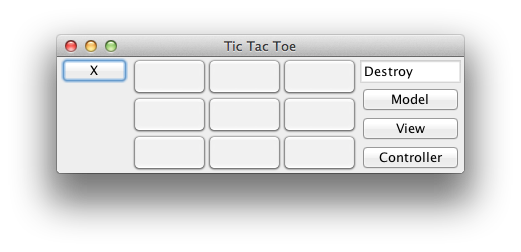
\includegraphics[scale=0.38]{TicTacToeScreenCut/0.png}
        }
        \subfloat[]{
           \label{fig:t1}
           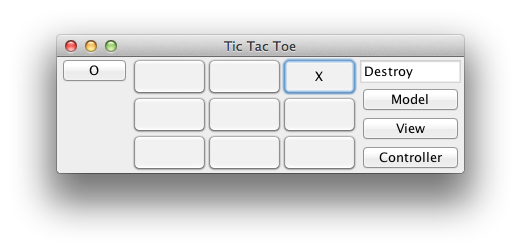
\includegraphics[scale=0.38]{TicTacToeScreenCut/1.png}
        }\\
        \subfloat[]{
            \label{fig:t2}
            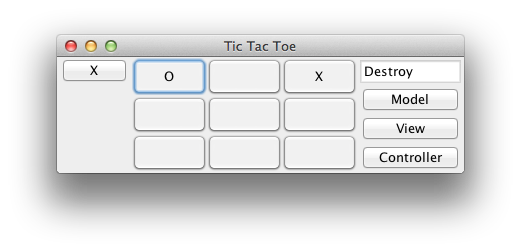
\includegraphics[scale=0.38]{TicTacToeScreenCut/2.png}
        }
        \subfloat[]{
            \label{fig:t3}
            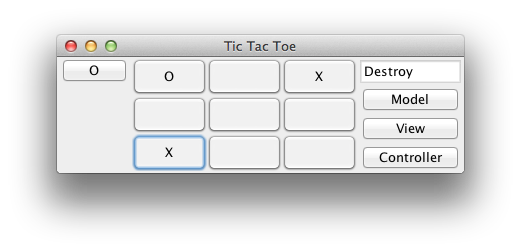
\includegraphics[scale=0.38]{TicTacToeScreenCut/3.png}
        }\\
        \subfloat[]{
            \label{fig:t4}
            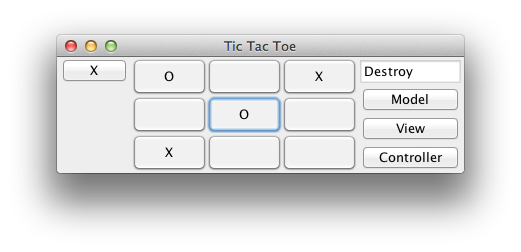
\includegraphics[scale=0.38]{TicTacToeScreenCut/4.png}
        }
        \subfloat[]{
           \label{fig:t5}
           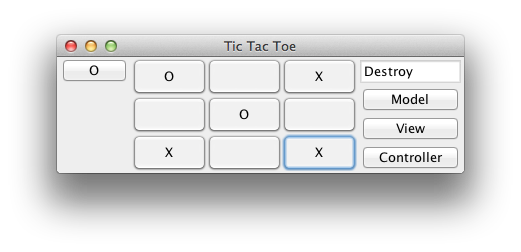
\includegraphics[scale=0.38]{TicTacToeScreenCut/5.png}
        }\\        
        \subfloat[]{
            \label{fig:t6}
            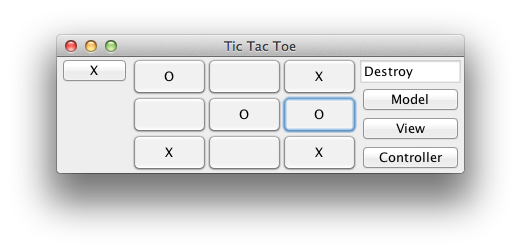
\includegraphics[scale=0.38]{TicTacToeScreenCut/6.png}
        }
        \subfloat[]{
           \label{fig:t7}
           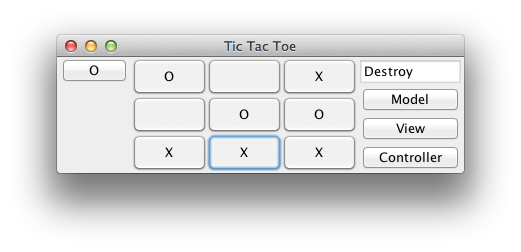
\includegraphics[scale=0.38]{TicTacToeScreenCut/7.png}
        }\\                
        \subfloat[]{
           \label{fig:t8}
           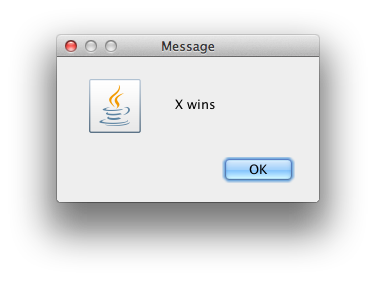
\includegraphics[scale=0.38]{TicTacToeScreenCut/8.png}
        }\\                        
    \end{center}
     \caption{A Game of Tic-Tac-Toe}
   \label{tictactoe_example}
\end{figure}


\subsubsection{The MVC pattern}

Model-view-controller (MVC) is a software architecture pattern introduced by 
\citet{reenskaug1979original}.  The pattern separates the data abstraction
(the model), the representation of data (the view), and the component for 
manipulating the data and interpreting user inputs (the controller).  
One key design principle of MVC is that the model and the view {\it never} 
communicate with each other directly.  Instead, the controller is responsible 
for coordinating the model and the view, for example,  sending instructions and 
reacting to messages from the model and the view.  

MVC has been widely used in the design of applications with a graphical user 
interface (GUI), from early Smalltalk programs written in Xerox Parc 
\citep{reenskaug1979original, reenskaug2003model}, to modern web application 
frameworks like the Zend framework \citep{allen2009zend}, to mobile 
applications including Apple iOS applications \citep{apple:objc}.  This 
section will follow the MVC pattern to implement a Tic-Tac-Toe Game with a 
GUI.  The challenge here is using types to prevent the 
situation where the model sends the controller a message expected from the 
view, or the view pretends to be the model. 
 


\subsection{A TAkka Implementation}




\begin{figure}[p]
\begin{lstlisting}[language=scala, escapechar=?]
package sample.tic_tac_toe.takka

?\textcolor{blue}{sealed trait ControllerMessage}?
?\textcolor{blue}{sealed trait View2ControllerMessage extends ControllerMessage}?
final case class ButtonClickedAt(row:Int, col:Int) extends View2ControllerMessage

?\textcolor{blue}{sealed trait Model2ControllerMessage extends ControllerMessage}?
final case class GridNotEmpty(row:Int, col:Int) extends Model2ControllerMessage
final case class PlayedCross(row:Int, col:Int) extends Model2ControllerMessage
final case class PlayedO(row:Int, col:Int) extends Model2ControllerMessage
final case class NextMove(move:Move) extends Model2ControllerMessage
final case class Winner(move:Move) extends Model2ControllerMessage

?\textcolor{blue}{sealed trait Controller2ViewMessage}?
final case class DisplyError(err:String) extends Controller2ViewMessage
final case class DrawCross(row:Int, col:Int) extends Controller2ViewMessage
final case class DrawO(row:Int, col:Int) extends Controller2ViewMessage
final case class DisplayNextMove(move:Move) extends Controller2ViewMessage
final case class AnnounceWinner(winner:Move) extends Controller2ViewMessage

?\textcolor{blue}{sealed trait Controller2ModelMessage}?
final case class MoveAt(row:Int, col:Int) extends Controller2ModelMessage

final case class ModelSetController(controller:ActorRef[Model2ControllerMessage]) extends Controller2ModelMessage
final case class ViewSetController(controller:ActorRef[View2ControllerMessage]) extends Controller2ViewMessage


sealed trait Move
final case object X extends Move
final case object O extends Move
\end{lstlisting}
\caption{TicTacToe: Message}
\label{TTT_message}
\end{figure}

\begin{figure}[p]

\begin{lstlisting}[language=scala, escapechar=?]
package sample.tic_tac_toe.takka
import takka.actor._
?\textcolor{blue}{final class Model extends Actor[Controller2ModelMessage]}? {
  ?\textcolor{blue}{var controller:ActorRef[Model2ControllerMessage]}? = _  
  def typedReceive = {
    case ModelSetController(control) => controller = control
    case MoveAt(row:Int, col:Int) =>   { model.setStatus(row, col)  }
  }  
  private object model {
    sealed trait GridStatus
    case object Empty extends GridStatus
    case object XModelMove extends GridStatus
    case object OModelMove extends GridStatus // Uppercase O
    
    var nextXMove:Boolean = true // true->X false->O    
    val status:Array[Array[GridStatus]] = 
          Array(Array(Empty, Empty, Empty),
                 Array(Empty, Empty, Empty),
                 Array(Empty, Empty, Empty))
    def setStatus(row:Int, col:Int) = {   
      if(nextXMove){
          if (status(row)(col) == Empty) {
            status(row)(col) = XModelMove
            controller ! PlayedCross(row, col)
            nextXMove = false
            controller ! NextMove(O)
          }else{  controller ! GridNotEmpty(row, col)          }
      }else{
          if (status(row)(col) == Empty) {
            status(row)(col) = OModelMove
            controller ! PlayedO(row, col)
            nextXMove = true
            controller ! NextMove(X)
          }else{  controller ! GridNotEmpty(row, col)          }     
      }

      checkWinner match {
        case Empty =>
        case XModelMove =>          controller ! Winner(X)
        case OModelMove =>          controller ! Winner(O)          
     }}
   def checkWinner:GridStatus = {
     // reuse GridStatus instead of a new set of values
     // return XModelMove if X wins
     // return OModelMove if O wins
     // return Empty if no winner has 
}}
\end{lstlisting}
\caption{TicTacToe: Model}
\label{TTT_model}
\end{figure}

\begin{figure}[p]
\begin{lstlisting}[language=scala, escapechar=?]
package sample.tic_tac_toe.takka

import takka.actor._
import scala.swing._
import scala.swing.event._
import javax.swing.JOptionPane

?\textcolor{blue}{final class View extends Actor[Controller2ViewMessage]}?{
  ?\textcolor{blue}{private var controller:ActorRef[View2ControllerMessage]}? = _
   
  private var guiApp:GUIApplication = _;
      
  def typedReceive = {
     case ViewSetController(control) =>
       assert(controller == null, "controller has been set")
       controller = control
       guiApp = new GUIApplication(controller)
       guiApp.main(Array(""))              
     case DisplyError(err) =>       guiApp.displayError(err)
     case DrawCross(row, col) =>       guiApp.draw(row, col, true)
     case DrawO(row, col) =>       guiApp.draw(row, col, false)
     case DisplayNextMove(move) =>       guiApp.showNextMove(move)
     case AnnounceWinner(winner:Move) => winner match{
       case X => guiApp.announceWinner(true)
       case O => guiApp.announceWinner(false)
     }
  }
}


class GUIApplication(controller:ActorRef[View2ControllerMessage]) extends SimpleSwingApplication {
   def draw(row:Int, col:Int, isCross:Boolean) { 
     // draw X or O at (row, col)
   }
   def showNextMove(move:Move) {
     // update next player
   }
   def displayError(err:String){
     // show error message
   }
   def announceWinner(isCross:Boolean){
     // announce winner
   }
}
\end{lstlisting}
\caption{TicTacToe: View}
\label{TTT_view}
\end{figure}


\begin{figure}[p]
\begin{lstlisting}[language=scala, escapechar=?]
package sample.tik_tak_tok.takka

import takka.actor._

?\textcolor{blue}{final class Controller(model:ActorRef[Controller2ModelMessage], view:ActorRef[Controller2ViewMessage]) extends Actor[ControllerMessage]}? {
  def typedReceive = {
    case ButtonClickedAt(row, col) =>
      model ! MoveAt(row, col)
    case GridNotEmpty(row, col) =>
      view ! DisplyError("grid "+row+" , "+col+" is not empty")
    case PlayedCross(row, col) =>
      view ! DrawCross(row, col)
    case PlayedO(row, col) =>
      view ! DrawO(row:Int, col:Int)
    case NextMove(move) =>
      view ! DisplayNextMove(move)
    case Winner(move) =>
      view ! AnnounceWinner(move)
  }
  
  override def preStart() = {
    model ! ModelSetController(typedSelf.publishAs[Model2ControllerMessage])
    view ! ViewSetController(typedSelf.publishAs[View2ControllerMessage])
  }
}

package sample.tic_tac_toe.takka

import takka.actor._
?\textcolor{blue}{object TicTacToeApplication extends App \{}?
  ?\textcolor{blue}{val system = ActorSystem("LocalTicTacToe")}?
  ?\textcolor{blue}{val model = system.actorOf(Props[Controller2ModelMessage, Model], "model")}?
  ?\textcolor{blue}{val view = system.actorOf(Props[Controller2ViewMessage, View], "view")}?
  ?\textcolor{blue}{val controller = system.actorOf(Props(new Controller(model, view)), "controller")  }?
?\textcolor{blue}{\}}?
\end{lstlisting}
\caption{TicTacToe: Application}
\label{TTT_controller}
\end{figure}

TAkka solves the type pollution problem by using subtyping polymorphism.  The code from 
Figure~\ref{TTT_message} to Figure~\ref{TTT_controller} gives an TAkka 
application that implements the Tic-Tac-Toe game with a GUI.  The code marked 
in \textcolor{blue}{blue} may be reused by other applications built 
using the MVC pattern.


Messages used in this implementation are given in Figure~\ref{TTT_message}. 
Messages sent to the controller are separated into two groups: those expected 
from the model and those expected from the view.  The {\tt Controller} actor of 
this application, defined in Figure~\ref{TTT_controller}, reacts to messages 
sent either from the {\tt Model} actor or the {\tt View} actor.  In its 
initialization process, however, the controller publishes itself as different 
types to the view actor and the model actor.  Although the {\tt publishAs} 
methods in line 22 and line 23 of Figure~\ref{TTT_controller} can be committed 
because the type of the controller has been refined in the {\tt 
ModelSetController} message and the {\tt ViewSetController} message, the code
explicitly expresses the type convention and lets the compiler double check the 
type.

In the definition of the {\tt Model} actor (Figure~\ref{TTT_model}) and the 
{\tt View} actor (Figure~\ref{TTT_view}), the {\tt Controller} actor is declared 
as different types.  As a result, both the view and the model only know the 
communication interface between the controller and itself.  The {\tt Model} 
actor internally represents the game board as a two dimensional array.  Each 
time the model receives a request from the controller, it updates the status of 
the board and then announce the winner or the next player to the controller.  
The {\tt View} actor maintains a GUI application that displays the game board 
and listens to user input.  All user input is forwarded to the controller 
which sends corresponding requests to the model.  When the view receives 
requests from the controller, it updates the game board or announce the winner 
via the GUI.  Detailed GUI implementation is omitted in this thesis for clarity.
Readers can found the complete code in the public code repository of this project. \citep{takka_repo}


Finally, setting up the application is straightforward.  In the code 
given at the bottom of Figure~\ref{TTT_controller}, a {\tt Model} actor, a 
{\tt View} actor, and a {\tt Controller} actor are initialized in a local actor 
system.  In this implementation, the controller actor must be initialized at the 
end because its initialization requires actor references of the model and the 
view.  The user interface of this application looks like the one gives in 
Figure~\ref{tictactoe_example}.  



\subsection{A Scala Interface}
\label{type_pollution_oo}



The type pollution problem is avoided in TAkka by publishing different types of 
an actor to different users.  This method can be applied to any language that 
supports polymorphism.  For example, Figure~\ref{TTT_interface} gives an 
interface of implementing the Tic-Tac-Toe game using the MVC pattern without actors.  The code 
marked in \textcolor{blue}{blue} can be modified for building other 
applications using the MVC pattern.

Similar to the TAkka implementation which separates the type of messages sent 
from a model to a controller and a view to a controller, the interface in Figure 
\ref{TTT_interface} separates the methods of a controller to be called by a 
model and those to be called by a view into two distinct traits.  The controller 
is defined as the subclass of both traits.

The example implementation, however, is difficult to maintain.  Notice that the 
{\tt ControllerForView} trait and the {\tt ControllerForModel} trait are the 
supertypes of the {\tt Controller} trait.  As a result, those two traits 
and their methods should be defined in advance.  Each time a new 
method shall be added to either of the two traits, 
the whole program needs to be recompiled and re-deployed.  Where an application 
is a collaborative project maintained by different groups, attempts at 
large-scale updates should be avoided whenever possible.  

In contrast, our TAkka implementation avoids the problems suffered by the simple
Scala solution because new messages can be added easily as a subtype
of an earlier defined message.   With the benefit of backward compatible behaviour upgrading (Section 
\ref{hot_swapping}), the controller, the model and the view can be updated 
separately.




\begin{figure}[p]
\begin{lstlisting}[language=scala, escapechar=?]
package sample.tic_tac_toe.mvcobject

?\textcolor{blue}{trait Controller extends ControllerForView with ControllerForModel}?
class GameController(model:Model, view:View) extends Controller {
  // implementation
}

?\textcolor{blue}{trait ControllerForView}? {
  def buttonClickedAt(row:Int, col:Int):Unit
}
?\textcolor{blue}{trait ControllerForModel}? {
  def gridNotEmpty(row:Int, col:Int):Unit
  def playedCross(row:Int, col:Int):Unit
  def playedO(row:Int, col:Int):Unit
  def nextMove(move:Move):Unit
  def winner(move:Move):Unit
}

?\textcolor{blue}{trait Model}? {
  ?\textcolor{blue}{def setController(controller:ControllerForModel): Unit}?
  def moveAt(row:Int, col:Int): Unit
}
class GameModel extends Model {
  // implementation
}

?\textcolor{blue}{trait View}? {
  ?\textcolor{blue}{def setController(controller:ControllerForView): Unit}?
  def displyError(err:String): Unit
  def drawCross(row:Int, col:Int): Unit
  def drawO(row:Int, col:Int): Unit
  def displayNextMove(move:Move): Unit
  def announceWinner(winner:Move): Unit
}
class GameView extends View {
  // implementation
}

sealed trait Move
final case object X extends Move
final case object O extends Move

?\textcolor{blue}{object TicTacToeApplication extends App \{}?
  ?\textcolor{blue}{val model = new GameModel;}?
  ?\textcolor{blue}{val view = new GameView;}?
  ?\textcolor{blue}{val controller = new GameController(model, view)  }?
?\textcolor{blue}{\}}?
\end{lstlisting}
\caption{TicTacToe: MVC Interface}
\label{TTT_interface}
\end{figure}

\newpage 

\section{Expressiveness}
\label{expressiveness}

To assess the expressiveness of the TAkka library.  The author 
selected examples from Erlang QuviQ \citep{quviq}
and open source Akka projects to ensure that the main requirements for actor 
programming were not unintentionally neglected.  Section~\ref{examples}
lists examples ported from other projects. Examples from Erlang 
QuviQ were re-implemented using both Akka and TAkka.  Examples from 
Akka projects were re-implemented using TAkka.   Section~\ref{results}
gives the evaluation results in term of code size and and type error
detection.

\subsection{Examples}
\label{examples}

\subsubsection{Examples from the QuviQ Project}

QuviQ \citep{quviq} is a QuickCheck tool for Erlang programs.  It generates 
random test cases according to specifications for testing applications written 
in Erlang.  QuviQ is a commercial product.  The author gratefully acknowledges 
Thomas Arts from QuviQ.com and Francesco Cesarini from Erlang Solutions 
for providing the Erlang source code for the ATM simulator example and the 
Elevator Controller example, two examples used in their commercial training 
courses.

The descriptions below reflects the design of the Akka and TAkka version ported 
from the Erlang source code.  This thesis will only describe the overall 
structure of those two examples.  For copyright reason, code for this example
is available in the private repository but is not available in the 
public repository.  Readers who would like to have access to the source 
code may contact the author or directly contact QuviQ.com and Erlang Solutions for their permissions.







\paragraph{ATM simulator} This example contains 5 actor classes.  It simulates 
a bank ATM system consisting of the following components:

\begin{itemize}
 \item a database backend that keeps records of all users.
 \item a front-end for the ATM with graphical user interface
 \item a controller for the ATM
\end{itemize}

Figure~\ref{atm}, cited from \citep{atmprivate}, gives the Finite State Machine 
that models the behaviour of the front-end of the ATM.


\begin{figure}[p]
     \begin{center}            
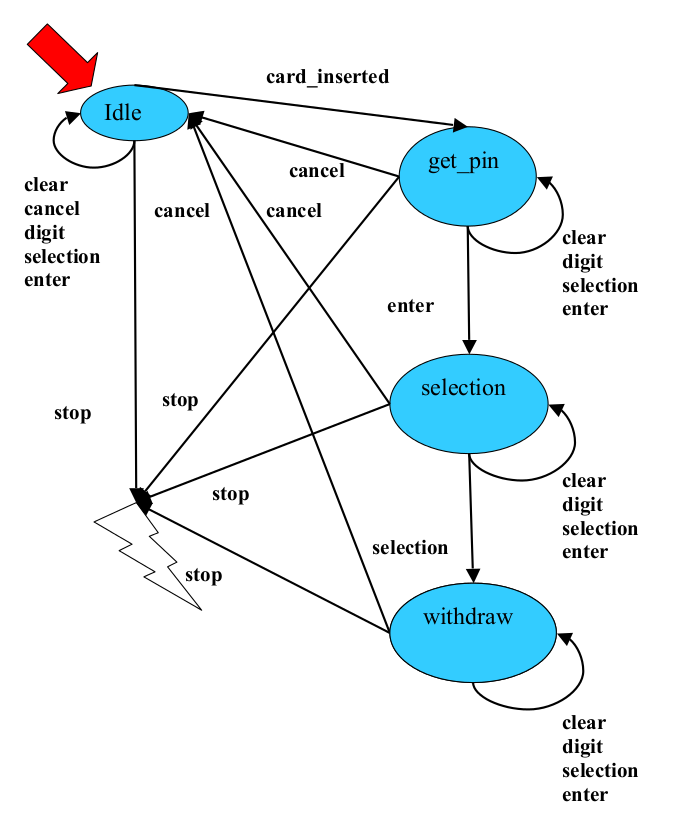
\includegraphics[keepaspectratio=true,height=0.6\paperheight]
{Pictures/ATM_FSM.png}
    \end{center}
     \caption{Example: ATM}
   \label{atm}
\end{figure}


\newpage
\paragraph{Elevator Controller}\ This example contains 7 actor classes.  It 
simulates a system that monitors and schedules a number of elevators.

Figure~\ref{elevator_controller} gives an example elevator controller that 
controls three elevators in a building that has 6 levels.  The three worker 
actors are:
\begin{itemize}
 \item The monitor class that provides a GUI.
 \item The elevator class that models a specific elevator.
 \item The scheduler class that reacts to user inputs.
\end{itemize}

The other 4 actors are supervisors for other components.  The example is 
shipped with QuickCheck properties that checks whether events generated by 
users are correctly handled.



\begin{figure}[p]
     \begin{center}
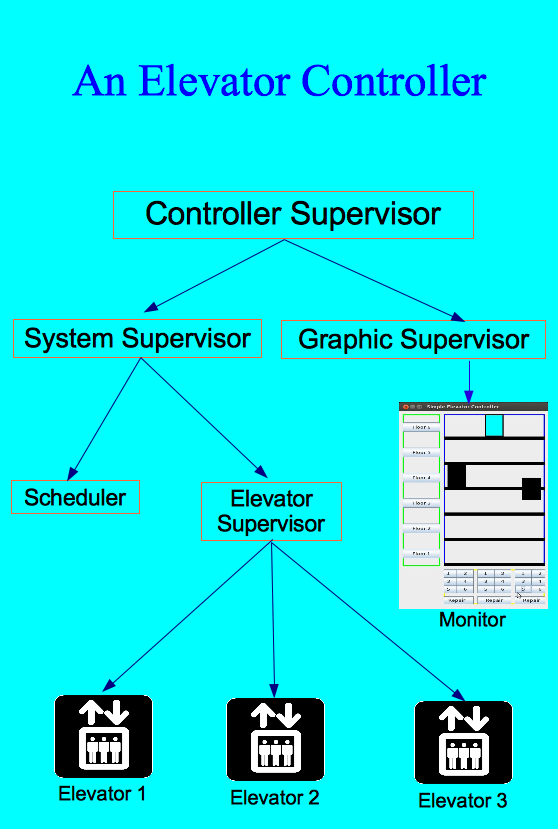
\includegraphics[keepaspectratio=true,height=0.6\paperheight]
{Pictures/ElevatorController.png}
    \end{center}
     \caption{Example:  Elevator Controller}
   \label{elevator_controller}   
\end{figure}

\subsubsection{Examples from the Akka Documentation}

The Akka Documentation \citep{akka_doc} contains some examples that demonstrate 
actor programming and supervision in Akka.  The author has ported the 
following examples to check that applications built using TAkka behave similarly 
to Akka applications.

\paragraph{Ping Pong} This example contains 2 actor classes: {\tt Ping} and 
{\tt Pong}.  The two actors send messages to each other a number of 
times and then terminate.  The example begins with a {\tt ping} message sent 
from a {\tt Ping} actor to a {\tt Pong} actor.  The {\tt Pong} actor replies a 
{\tt pong} message when it receives a {\tt ping} message.  When a {\tt Ping} 
actor receives a {\tt pong} message, it updates its internal message counter.  
If the message counter does not exceed a set number, it sends another {\tt 
Ping} message, otherwise the program terminates.



\paragraph{Dining Philosophers} This example contains 2 actor classes.  It 
models the dining philosophers problem \citep{wiki:philosophers} using 
Finite State Machines (FSMs).   The Dining Philosophers problem is one of the 
classical problems that exhibit 
synchronization issues in concurrent programming.  In the ported version five 
philosophers sit around a table with five chopsticks interleaved.  Each 
philosopher alternately thinks and eats.  Before starting eating, a philosopher 
needs to hold chopsticks on both sides.  At any time, a chopstick can only be 
held by one philosopher.  A philosopher puts down both chopsticks when he 
finishes eating and thinks for a random period.  




\paragraph{Distributed Calculator} This example contains 4 actor classes.  
It demonstrates distributed computation and dynamic behaviour update on the 
receive function of an actor.  The TAkka version of this example is used as a 
case study in Section~\ref{sec_distributed_calculator}.

\paragraph{Fault Tolerance} This example contains 5 actor classes.  It models 
simple key-value data storage.  The data storage maps {\tt String} keys to 
{\tt Long} values.  The data storage throws a {\tt StorageException} when 
users try to save a value between 11 and 14.  The data storage service is 
supervised using the {\tt OneForOne} supervisor strategy.


\subsubsection{Examples from Other Open Source Projects}

The QuviQ examples and the Akka documentation examples are demonstration 
examples for training purposes.  This thesis further ports the following 
examples from open source projects to enlarge the scope of the test.

\paragraph{Barber Shop}  This application has 6 actor classes.  The Akka 
version of this example is implemented by \citet{BarberShop}.  This example
application models the sleeping barber problem \citep{wiki:barber}, which 
involves inter-process communication and synchronization.

\paragraph{EnMAS} This medium size project has 5 actor classes.  The EnMAS 
project, which stands for Environment for Multi-Agent Simulation, is a framework 
for multi-agent and team-based artificial intelligence research \citep{EnMAS}.  
Agents in this framework are actors while specifications are written in DSL 
defined in Scala.


\paragraph{Socko Web Server} The implementation of this application contains 
4 actor classes.  Socko \citep{SOCKO} is a lightweight Scala web server that 
can serve static files and support RESTful APIs.  

\paragraph{Gatling}  This application contains 4 actor classes.  Gatling  
\citep{Gatling} is a stress testing tool for web applications.  It uses actors 
and synchronous I/O methods to improve its efficiency.  The application is 
shipped with a tool that reports test results in graphical charts.

\paragraph{Play Core} The core library of the Play framework only has 1 actor 
class.  The Play framework \citep{play_doc} is part of the TypeSafe stack for 
building web applications.  The Play project is actively maintained by 
developers at TypeSafe Inc. and in the Play community.  Therefore, this project 
only ports its core library which is also updated less frequently.
Because the original Akka Play is an active project on GitHub, a separate repository is 
forked for the TAkka version \citep{takka_play} so that updating non-core components is easier.





\subsection{Evaluation Results}
\label{results}

\subsubsection{Code Size}

This section investigates whether the type discipline enforced by TAkka restricts the 
expressibility of Akka.  Table~\ref{express} lists the examples used for expressiveness checks.  
Medium-seized examples are selected from Quviq \citep{quviq}
and open source Akka projects to ensure that the main requirements for actor 
programming are not unintentionally neglected.  Examples from 
Quviq are re-implemented using both Akka and TAkka.  Examples from 
Akka projects are re-implemented using TAkka.  Following standard practice \citet{Fleming} and \citet{HePa06},  
the author assesses the overall code modification and code 
size by calculating the geometric mean of all examples. The evaluation results 
in Table~\ref{express} show that when porting an Akka program to TAkka, about 
8.5\% lines of code need to be modified including additional type declarations. 
Sometimes, the code size can be smaller because TAkka code does not 
need to handle unexpected messages.  On average, the total program size 
of Akka and TAkka applications are almost the same.  Figure~\ref{fig:expressiveness}
reports the same result in a Scatter chart.



\begin{sidewaystable}[clockwise, p]
\begin{tabular}{| p{4.5 cm} | p{5.6 cm} | c | c |  c | c | c |}
\hline

Source & Example & \specialcell{Akka Code \\ Lines} &
\specialcell{Modified\\ TAkka Lines} & \specialcell{\% of \\Modified Code} &
\specialcell{TAkka Code\\ Lines}
& \specialcell{\% of \\Code Size} \\
\hline
Small   & String Processor & 25 & 11 & 44 & 22 & 88 \\
\cline{2-7}                            
Examples                            & Supervised Calculator &38 & 11 & 29 & 41 & 108 \\ 
\cline{2-7}
                            & Behaviour Upgrade & 38 & 10 & 26 & 39 & 102 \\
\cline{2-7}                            
                            & NQueens & 235 & 6 & 3 & 236 & 100 \\
\cline{2-7}                            
\hline

BenchErl  & bang & 93 & 8 & 8.6 & 94 & 101 \\
\cline{2-7}
Examples                            & big & 93 & 10 & 11 & 100 & 108 \\
\cline{2-7}                            
                            & ehb &201 & 23 & 11 & 216 & 107 \\ 
\cline{2-7}                            
                            & genstress &129 & 12 & 9.3 & 129 & 100 \\ 
\cline{2-7}                            
                            & mbrot & 125 & 8 & 6 & 130 & 104 \\
\cline{2-7}                            
                            & parallel &101 & 9 & 8.9 & 101 & 100 \\ 
\cline{2-7}                            
                            & ran & 98 & 8 & 2.6 & 101 & 103 \\
\cline{2-7}       
                            & serialmsg & 146 & 20 & 14 & 146 & 100 \\
\cline{2-7}       

\hline
QuviQ   & ATM simulator & 1148 & 199 & 17.3 & 1160 & 101 \\
\cline{2-7}
\citep{quviq}    & Elevator Controller & 2850 & 172 & 9.3 & 2878 & 101 \\
\hline
                     & Ping Pong & 67 & 13 & 19.4 & 67 & 100 \\
\cline{2-7}
Akka Documentation   & Dining Philosophers & 189 & 23 & 12.1 & 189 & 100  \\
\cline{2-7}
\citep{akka_doc}     & Distributed Calculator  & 250 & 43 & 17.2 & 250 & 100 \\
\cline{2-7}
                     & Fault Tolerance & 274 & 69 & 25.2 & 274 & 100 \\
\hline

               & Barber Shop \citep{BarberShop}& 754 & 104 & 13.7 & 751 & 99 \\
\cline{2-7}
Other Open Source    & EnMAS \citep{EnMAS} & 1916 & 213 & 11.1 & 1909 & 100 \\
\cline{2-7}
Akka Applications    & Socko Web Server \citep{SOCKO}  & 5024 & 227 & 4.5 & 
5017 & 100 \\
\cline{2-7}
                     & Gatling \citep{Gatling} & 1635 & 111 & 6.8 & 1623 & 99 \\
\cline{2-7}
              & Play Core \citep{play_doc} & 27095 & 15 & 0.05 & 27095 & 100 \\
\hline
geometric mean                   & & 319.5 & 27.4 & 8.6 & 324.4 & 101.5 \\
\hline
\end{tabular}
\caption{Expressiveness Evaluation}
\label{express}
\end{sidewaystable}

\begin{figure}[h]
     \begin{center}
        \subfloat[Code Size: Absolute Lines]{
            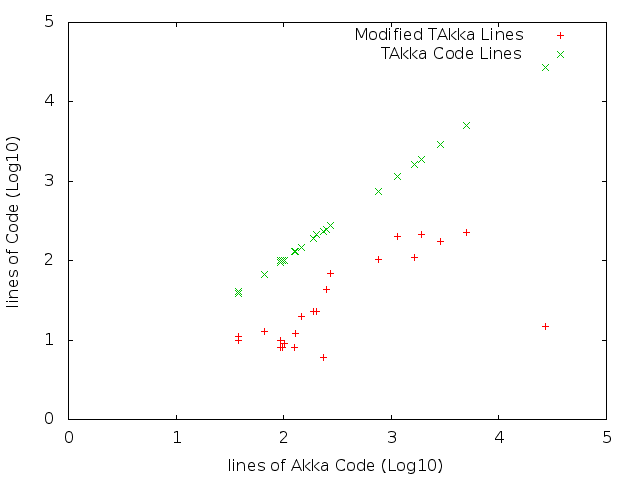
\includegraphics[scale=0.32]{Expressiveness/Expressiveness1.png}
        }
        \subfloat[Code Size: Relative Lines]{
           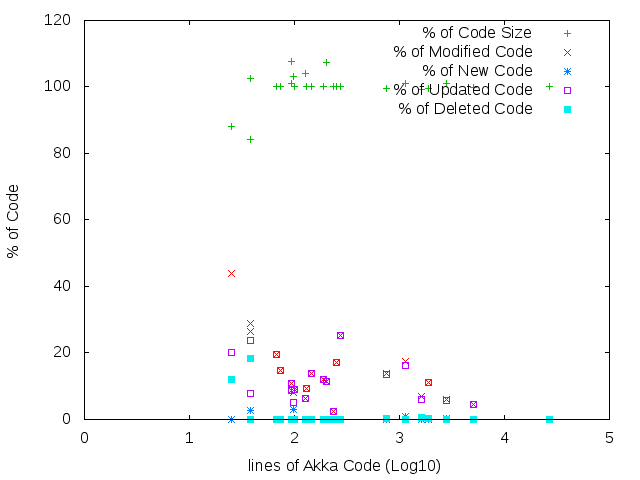
\includegraphics[scale=0.32]{Expressiveness/Expressiveness2.png}
        }
    \end{center}
    \caption{Code Size Evaluation}
   \label{fig:expressiveness}
\end{figure}

\subsubsection{Type Error}

A type error is reported by the compiler when porting the Socko example 
\citep{SOCKO} from its Akka implementation to an equivalent TAkka 
implementation.
Socko is a library for building event-driven web services.  The Socko designer
defines a {\tt SockoEvent} class to be the supertype of all events.  One
subtype of {\tt SockoEvent} is {\tt HttpRequestEvent}, representing events
generated when an HTTP request is received. The designer further implements
subclasses of {\tt Method}, whose {\tt unapply} method intends to pattern
match {\tt SockoEvent} to {\tt HttpRequestEvent}.  The Socko
designer made a type error in the method declaration so that the {\tt unapply}
method pattern matches {\tt SockoEvent} to {\tt SockoEvent}. The type error is
not exposed in test examples because those examples always pass instances 
of {\tt HttpRequestEvent} to the {\tt unapply} method and send the returned
values to an actor that accepts messages of {\tt HttpRequestEvent} type.
Fortunately, the design flaw is exposed when upgrading the Socko implementation 
using TAkka.



\section{Throughput}
\label{throughput}

The Play example \citep{play_doc} and the Socko example \citep{SOCKO} used in 
Section~\ref{expressiveness} are two frameworks for building web services in 
Akka.  A scalable implementation of a web service should be able to have 
a higher maximum throughput when more web servers are added.  Throughput is 
measured by the number of correctly handled requests per unit of time.

The JSON serialization example from the TechEmpower Web Framework benchmarks 
\citep{techempower} checks the maximum throughput achieved during a test.  This 
example is used in this thesis to test how the maximum throughput changes when 
adding more web server applications implemented using Akka Play, TAkka 
Play, Akka Socko, and TAkka Socko.  

For a valid HTTP request sent to path {\tt /json}, e.g. the one given in Figure 
\ref{json_request}, the web service should return a JSON serialization of a new 
object that maps the key message to the value ``Hello, World''.  JSON, which 
stands for JavaScript Object Notation, is a language independent format for 
data exchange between applications \citep{json}.  Figure~\ref{json_response} 
gives an example of an expected HTTP response.  The body of the example 
response, line 7, is the expected JSON message.


\lstset{language=html}

\begin{figure}[!h]
\begin{center}
  \subfloat[An Example HTTP Request]{%
  \label{json_request}
  \lstinputlisting{code/json_request}%
}
\hfill
  \subfloat[An Example HTTP Response]{%
  \label{json_response}
  \lstinputlisting{code/json_response}%
}
  \caption{Example: JSON serialization Benchmark}
\end{center}    
  \label{json_example}
\end{figure}
\lstset{language=scala}


All four versions of the web service were deployed to servers on Amazon 
Elastic Compute Cloud (EC2) \citep{ec2}.  The example was tested with up to 16 
EC2 micro instances (t1.micro), each of which had 0.615 GB Memory.   The author 
expected that web servers built using an Akka-based library and a TAkka-based 
library would have similar throughput.


To avoid pitfalls mentioned in \citep{pitfall}, a FreeBench \citep{freebench} 
tool was designed and implemented for benchmarking throughputs of HTTP 
servers.  One feature of the FreeBench tool is that it can benchmark web 
servers deployed at multiple addresses.  In the JSON serialization benchmark, 
the maximum throughput achieved when using the Elastic Load Balancing (ELB) 
service \citep{elb} did not obviously increase when more servers were added. 
In contrast, when all deployed EC2 servers were benchmarked, the 
total throughput increased slightly. One possible explanation for the above 
observation is that the benchmark is bounded by the throughput of ELB,
which runs on a micro EC2 instance.  Another 
feature of the FreeBench tool is that it can be configured to carry out a 
number of benchmarks in parallel and repeat the parallel benchmark a 
certain number of times.  The benchmark results of all tests are sent to a data 
store which reports a customised statistical summary.

The parameters set in this example were the number of EC2 instances used.  For 
each of the four types of server, the example was tested with up to 16 
EC2 instances.  For each number of EC2 instances, 10 rounds of benchmarking 
were executed. In each round, 20 sub-benchmarks were carried out in parallel to 
maximise the utility of broadband.  For each sub-benchmark, 10,000 requests were
sent.  The upload and download speed were manually monitored to confirm that 
the network speed was stable for most of the time during the test with the 
above configurations.

Figure~\ref{fig:throughput} summarises the results of the JSON serialization 
benchmark.  It shows the average and the standard deviation of the throughput 
in each test.  The result shows that web servers built using an Akka-based 
library and a TAkka-based library have similar throughput.  The micro example
used in this test does not show a good throughput scalability in both Akka
and TAkka versions.  It will be more interesting if we can benchmark on a real Akka web service
whose throughput is linear to the number of available servers.






\begin{figure}[h]
     \begin{center}
        \subfloat[]{
            \label{fig:play_throughput}
            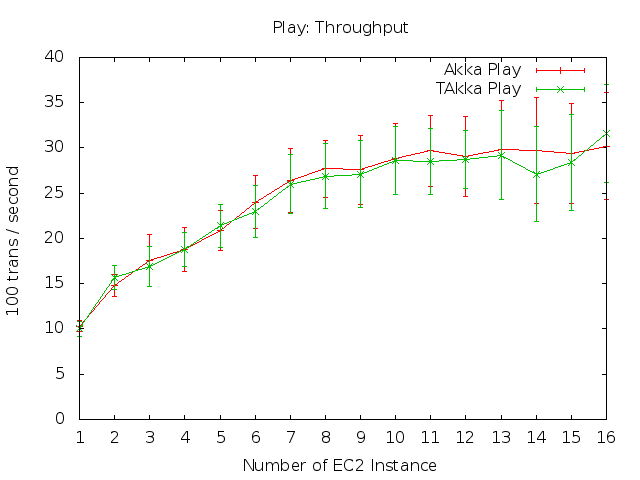
\includegraphics[scale=0.32]{Play_throughput.png}
        }
        \subfloat[]{
           \label{fig:socko_throughput}
           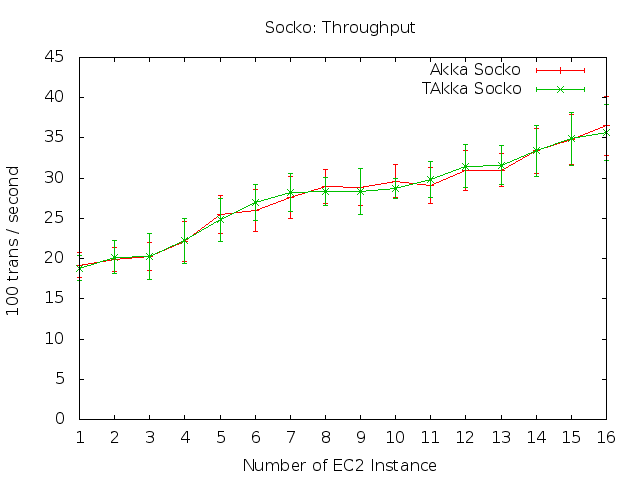
\includegraphics[scale=0.32]{Socko_throughput.png}
        }
    \end{center}
     \caption{Throughput Benchmarks}
   \label{fig:throughput}
\end{figure}

\newpage
\section{Efficiency and Scalability}
\label{efficiency}




The TAkka library is built on top of Akka so that code for shared features 
can be re-used.  The main sources of overheads in the TAkka implementation
are:

\begin{enumerate}[i)]
  \item the cost of adding an additional operational layer on top of Akka 
code,
  \item the cost of constructing type descriptors,
  \item the cost of transmitting type descriptors in distributed settings, and
  \item the cost of dynamic type checking when registering new typed names.
\end{enumerate}

The upper bounds of costs i) and ii) were assessed by a micro 
benchmark which assessed the time for initializing {\it n} instances of {\tt 
StringCounter} defined in Figure~\ref{fig:akka_string_counter} and Figure 
\ref{takka_string_counter}. When {\it n} ranges from $10^4$ to $10^5$, as 
shown in Figure~\ref{cost_of_type}, the TAkka implementation runs roughly 
half as fast as the Akka implementation.  


\vspace{15pt}
\begin{figure}[h]
\begin{center}
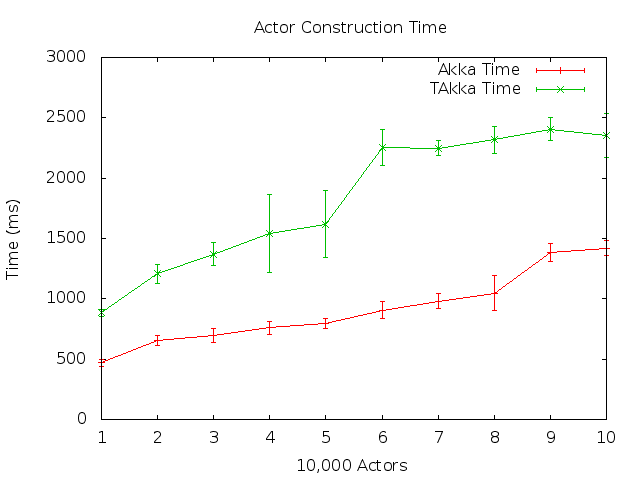
\includegraphics[scale=0.6]{efficiency/Actor_Construction.png}
\caption{Cost of Actor Construction}
\label{cost_of_type}
\end{center}
\end{figure}

\newpage

The cost of transmitting a type descriptor should be close to the cost of 
transmitting the string representation of its fully qualified type name.  The 
relative overhead of the latter cost depends on the cost of computations 
spent on application logic.

TAkka applications that have a relatively heavy computation cost should have 
similar runtime efficiency and scalability compared with equivalent Akka 
applications because static type checking happens at compile time and dynamic 
type checking is usually not the main cost of applications that involve other 
meaningful computations.  To confirm the above expectation, the speed-up of 
multi-node TAkka applications was further investigated by porting 
appropriate micro benchmark examples from the BenchErl benchmarks in the 
RELEASE project \citep{RELEASE, aronis2012scalability}. 


\subsection{BenchErl Overview}
\label{bencherl_overview}

BenchErl \citep{RELEASE, aronis2012scalability} is a scalability benchmark suite 
for applications written in Erlang.  It includes a set of micro benchmark 
applications that assess how an application changes its performance when 
additional resources (e.g. CPU cores, schedulers, etc.) are added.  This thesis 
uses BenchErl examples, which do not involve OTP ad-hoc libraries, to 
investigate how the performance of an application changes when more distributed 
nodes are added.

All BenchErl examples are implemented in a similar structure.  Each BenchErl 
benchmark spawns one master process and a configurable number of child 
processes.  Child processes are evenly distributed across available 
potentially distributed nodes.  The master process asks each child process to 
perform a task and send the result back to the master process.  Finally, when 
results are collected from all child processes, the master process assembles 
them and reports the overall elapsed time for the benchmark.

BenchErl examples have similar structure to the MapReduce model 
\citep{dean2008mapreduce}, which matches many real world tasks.  More 
importantly, those programs are automatically parallelized when executed on 
a cluster of machines.  This pattern allows benchmark users to focus on the 
effects of changes in computational resources rather than specific 
parallelization and scheduling strategies of each example.






\newpage

\subsection{Benchmark Examples}

\subsubsection{Ported BenchErl Examples}
\label{ported_examples}

The following BenchErl examples were ported for comparing the efficiency 
and scalability of applications built using TAkka and Akka:

\paragraph{bang}  This benchmark tests many-to-one message passing.  The child 
processes spawned in this example are {\it sender} actors which send the 
master process a fixed number of dummy messages.  The master process 
initializes a counter, set to the product of the number of processes and the 
number of messages expected from each child.  When a dummy message is received, 
the master counts down the number of remaining expected messages.  The 
benchmark example completes when all expected messages are received.  

Parameters set in this example are the number of available nodes, the 
number of child processes to spawn, and the number of messages sent by each 
child process.  Instead of carrying out computations, the main task of this 
benchmark is sending messages from child processes to the master process.  
Therefore, the benchmark is likely to be bounded by throughput of the master node.


\paragraph{big}  This benchmark tests many-to-many message passing.  A child 
process in this example sends a {\tt Ping} message to each of the other child 
processes.  Meanwhile, each child replies with a {\tt Pong} message when it 
receives a {\tt Ping} message.  Therefore, if $n$ child processes are spawned, 
each child is expected to send $n-1$ messages and receive $n-1$ messages from 
others.  When a child completes the task, it sends a {\tt BigDone} message to 
the master actor.  The benchmark example completes when the master actor 
receives {\tt BigDone} messages from all of its children.  

Parameters set in this example are the number of available nodes and the number 
of child processes to spawn.  The main task of 
this benchmark is sending messages rather than computations.  For each child 
process, the number of messages it sends and receives is linear to the total 
number of child processes.  Similarly to the {\tt bang} example, the benchmark 
is likely to be bounded by throughput of the master node.


\paragraph{ehb} This benchmark re-implements the hackbench example 
\citep{hackbench} originally used for stress testing Linux schedulers.  
Each child process in this benchmark is a group of message senders and 
receivers.  Each sender sends each receiver a dummy message and waits for an 
acknowledge message.  Each sender repeats the process a number of times.  
When a sender has received all expected replies, it reports to the child actor 
that it has completed its task.  When all senders in the group have completed 
their tasks, the child process sends a complete message to the master process.  
The benchmark completes when all child processes have finished their tasks. 

Parameters set in this example are the number of available nodes, the number 
of groups, group size, and the number of loops.  Let $n$ be the number of 
groups in this benchmark, and $m$ be the number of senders and receivers in 
each group.  The master process then expects $n$ messages while a total of 
$2m^2$ messages are sent in each group.  Therefore, the main task of this 
benchmark is sending messages inside each group.  When the number of
available nodes to share the task of child processes is increased, this 
benchmark is expected to have shorter runtime.


\paragraph{genstress}  This benchmark is similar to the bang test.  It spawns an
echo server and a number of clients.  Each client sends some dummy messages to
the server and waits for its response.  When a client receives the response, 
it sends an acknowledge message to the master process.  The benchmark completes 
when results from all child processes are received.  There are two versions 
in Erlang, one using the OTP {\it gen\_server} behaviour, the other 
implementing a simple server-client structure manually.  This 
benchmark ports the version not using {\it gen\_server}.  

Parameters set in this example are the number of available nodes, the number 
of child client processes to spawn, and the number of messages sent by each 
child process. The main task of this benchmark is sending messages from child 
processes to the master process. Therefore, the benchmark is likely to be bounded by throughput of the master node.

\paragraph{mbrot} This benchmark models pixels in a 2-D image of a specific 
resolution.  For each pixel at a given coordinate, the benchmark determines 
whether it belongs to the Mandelbrot set \citep{wiki:mandelbrot} or not. The 
determination process usually requires a large number of iterations.  In this 
benchmark, child processes share roughly the same number of points.  The 
benchmark completes when all child processes have finished their tasks.

Parameters set in this example are the number of available nodes, the number 
of child processes to spawn, and the dimensions of the image.  Keeping the 
dimensions of the image to be a medium fixed size, with more available nodes to 
share the computation task, this benchmark is expected to have shorter runtime.




\paragraph{parallel}  This benchmark spawns a number of child processes.  Each 
child process creates a list of $N$ timestamps and checks that elements of the 
list are strictly increased, as promised by the implementation of the {\it now} 
function.  After completing the task, the child process sends the result list 
to the master process.  The benchmark completes when results from all child 
processes are received.

Parameters set in this example are the number of available nodes, the number of 
child processes, and the number of timestamps each child creates. Compared to 
the cost of creating timestamps and comparing data locally, the cost of sending 
distributed messages is usually much higher.  Therefore, the runtime of this 
benchmark is likely to be bounded by the task of sending results to the 
master process.




\paragraph{ran}  This benchmark spawns a number of processes.  Each child 
process generates a list of 100,000 random integers, sorts the list using 
quicksort, and sends the first half of the result list to the master process.  
The benchmark completes when results from all child processes are received.

Parameters set in this example are the number of available nodes and the 
number of child processes to spawn. For each child process, the cost of 
generating integers is linear to the number of integers, and the cost of 
sorting is linear logarithmically to the number of integers.  If the number of 
generated integers in each child process is increased so that the cost of 
communicating with the master process can be neglected, this benchmark is a 
good example for a scalability test.  Unfortunately, the space cost of this 
example also increases when the number of generated integers is increased.  In 
the TAkka and Akka benchmarks, the cost of garbage collection by JVM cannot be 
neglected when the number of generated integers is set to a higher number.


\paragraph{serialmsg} This benchmark tests message forwarding through a
dispatcher.  This benchmark spawns one proxying process and a number of 
pairs of message generators and message receivers.  Each message 
generator creates a random short string message and asks the proxying process 
to forward the message to a specific receiver.  A receiver sends the master 
process a message when it receives the message.  The benchmark completes when 
the master process receives messages from all receivers.

The parameters set in this example are the number of available nodes, the 
number of pairs of senders and receivers,  the number of messages and the 
message length.  Clearly, this benchmark is bounded by the throughput
of the proxying process when the speed of 
generating messages exceeds the speed of forwarding messages.


\subsubsection{BenchErl Examples that are Not Ported}

The following BenchErl examples are not ported for reasons given in respective 
paragraphs.

\paragraph{ets\_test} ETS table is an Erlang build-in module for concurrently 
saving and fetching shared global terms  \citep{ErlangManual}.  This benchmark 
creates an ETS table.  Child processes in this benchmark perform insert and 
lookup operations to the created ETS table a number of times.  This example 
is not ported because it uses ETS table, a feature that is specific to the 
Erlang OTP platform.

\paragraph{pcmark} Similarly to the {\it ets\_test} example, this benchmark 
also tests ETS operations.  In this benchmark, five ETS tables are created. 
Each created table is filled with some values before the benchmark begins.  The 
benchmark spawns a certain number of child processes that read the content of 
those tables.  This example is not ported either because it uses the ETS table.


\paragraph{timer\_wheel} Similarly to the {\it big} example, this benchmark 
spawns a number of child processes that exchange ping and pong messages.  
Differently to the {\it big} example, processes in this example can be 
configured to await reply messages only for a specified timeout.  In cases where 
no timeout is set, or it is set to a short period, this example is the same 
as the {\it big} example.  If a timeout is set to a long period, the 
runtime of this example is bounded by the timeout.  For the above reason, this 
example is not ported.



\newpage


\subsection{Benchmark Methodology}
\subsubsection{Testing Environment}

The benchmarks were run on a 32 node Beowulf cluster at Heriot-Watt 
University.  The 32 Beowulf cluster nodes each comprise eight Intel 5506 cores 
running at 2.13GHz. All machines run under Linux CentOS 5.5. The Beowulf 
nodes are connected with Baystack 5510-48T switches with 48 10/100/1000 ports.

\subsubsection{Determining Parameters}
\label{bench_parameters}

The main interest of the efficiency and scalability test is to check whether 
applications built using Akka and TAkka have similar efficiency and 
scalability.  Meanwhile, our secondary interest is to know how 
the required run-time of a BenchErl example changes when more 
machines are employed.  Ideally, for each comparison on the efficiency of 
an Akka application and its equivalent TAkka application, the only variable 
should be the number of employed nodes.  Nevertheless, the BenchErl examples 
listed in Section~\ref{ported_examples} have more parameters to be configured.  
Experiments for our main interests can be carried out with any 
parameters, however; for consideration of our secondary interest, 
parameters for each example were selected according to the following three 
criteria:

First, except for the RAN example, the runtime of each experiment was 
constrained to be 40 seconds.  The decision was made so that the time to 
measure each example was acceptable.  As will be explained in the next 
section, each example was tested for a total of 90 rounds of experiments.  
Another reason for this decision was that the experiment should be able to 
complete in a reasonably short time when running on a single machine.  During 
the experiment, the author observed some configurations such that an example 
had a bad performance when run on a single machine but sped up by a factor 
bigger than the total number of available nodes when run with more nodes.  
These experiments give interesting results that proved the importance of 
distributed programming; however, it is desired that the number of nodes be the 
only independent variable throughout all experiments.  Therefore, the 
benchmarks preferred configurations that neglected the impact of other factors 
such as garbage collection.

Second, the benchmarks preferred configurations that had more workload for each 
child process. In a number of tests to determine parameters, the author 
observed employing more machines only had runtime benefit for those 
BenchErl examples whose runtime is bounded by the computational tasks rather 
than the throughput of the only master process.

Third, the benchmarks preferred configurations that had more child processes 
but did not violate the above two principles.  The benchmark was run on 
a maximum of 32 Beowulf machines.  Although each machine has 8 CPU cores, the 
number of CPU cores used to execute Akka and TAkka applications is not 
guaranteed.  For each example, it is started with a small number of child 
processes.  If the child process could have a higher workload by setting other 
parameters, other parameters were changed until the configuration violated the 
first criterion.  If the number of child processes and the number of available 
nodes were the only two parameters, or the workload of each child process did 
not change significantly with other possible configurations, the number of child 
processes was increased gently until the example took a long time to be 
completed on a single machine.

Based on the results of trial experiments, the parameters used in each 
example were as follows:

\paragraph{bang} 

\begin{itemize}
  \item number of child processes: 512
  \item number of messages sent by each child process: 2000
\end{itemize}

\paragraph{big} 
\begin{itemize}
  \item number of child processes: 1024
\end{itemize}

\paragraph{ehb}  

\begin{itemize}
  \item number of groups: 128
  \item group size: 10
  \item number of loops: 3
\end{itemize}

\paragraph{genstress}  

\begin{itemize}
  \item number of child processes: 64
  \item number of messages sent by each child process: 300
\end{itemize}


\paragraph{mbrot} 

\begin{itemize}
  \item number of child processes: 256
  \item dimensions of the image: 6000x6000
\end{itemize}


\paragraph{parallel}

\begin{itemize}
  \item number of child processes: 256
  \item number of timestamps each child to create: 6000
\end{itemize}



\paragraph{ran} 
\begin{itemize}
  \item number of child processes: 6000
  \item list size: 100000
\end{itemize}


\paragraph{serialmsg}

\begin{itemize}
  \item number of pairs of senders and receiver: 256
  \item number of messages: 100
  \item message size: 200 characters
\end{itemize}

\subsubsection{Measurement Methodology}

After determining the benchmark parameters for each example, the runtime of 
each program was measured as follows.  First, each benchmark contains nine 
tests that use different numbers of Beowulf nodes.  The number of nodes 
used in the benchmarks were 1, 4, 8, 12, 16, 20 , 24, 28, and 32.  Similarly 
to the Benchmark Harness process in \citep{blackburn2006dacapo}, test results 
was recorded after a number of dry-runs to warm-up the runtime environment.  
After the warm-up period, the test was run 10 times.  The 
run time was recorded for later analysis.  Following guidance given by 
\citet{Fleming} and \citet{HePa06}, the efficiency of each example 
using a specific number of nodes is reported by giving the average and standard 
deviation of the 10 runs.  The speed-up of a benchmark example using $n$ nodes 
is measured as the proportion of the average time with one node and the average 
time with $n$ nodes.  After each test, the runtime environment was cleaned up  
before changing the number of nodes or switching to another benchmark example.

\subsection{Evaluation Results}

The records of the BenchErl benchmarks are summarised in Figure 
\ref{runtime_efficiency}.  The efficiency results include both the average 
runtime and the standard deviation.  The scalability results are computed based 
on the average runtime.  The author observes the following though benchmarking:

\paragraph{Observation 1} In all examples, TAkka and Akka implementations had 
almost identical run-times and hence have similar scalability.  In Figure 
\ref{runtime_efficiency}, the runtime of Akka benchmarks and TAkka benchmarks 
often overlay each other.  For benchmarks that do not overlay, the 
difference is less than 10\% on average.  The scalability of Akka applications 
and the scalability of their TAkka equivalents appear slightly different 
because their differences are amplified by their runtime differences when 
running on a single node.

\paragraph{Observation 2} Some benchmarks scale well when more nodes are added. 
 Examples of this observation are the {\tt EHB} example and the {\tt MBrot}. 

\paragraph{Observation 3} Some benchmarks only scale well when a small number 
of nodes are added.  These examples do not scale when the number of nodes are 
greater than a certain number.  Examples of this observation are the {\tt Bang} 
example, the {\tt Big} example, and the {\tt Ran} example.  The speed-up of 
those examples does not further increase when the number of nodes is more than 
four or eight.  

\paragraph{Observation 4} Some benchmarks do not scale.  Examples of this 
observation are the {\tt GenStress} example and the {\tt Parallel} 
example, and the {\tt SerialMsg} example.




\begin{figure}[p]
     \begin{center}
        \subfloat[Bang Time]{
            \label{fig:1a}
            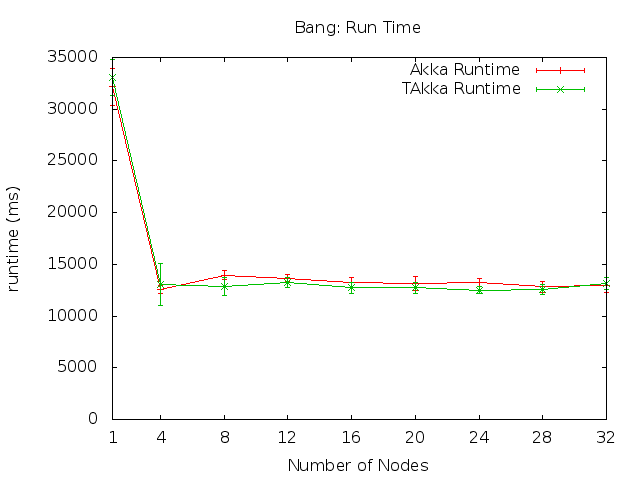
\includegraphics[scale=0.31]{efficiency/Bang_time.png}
        }
        \subfloat[Bang Scalability]{
           \label{fig:1b}
           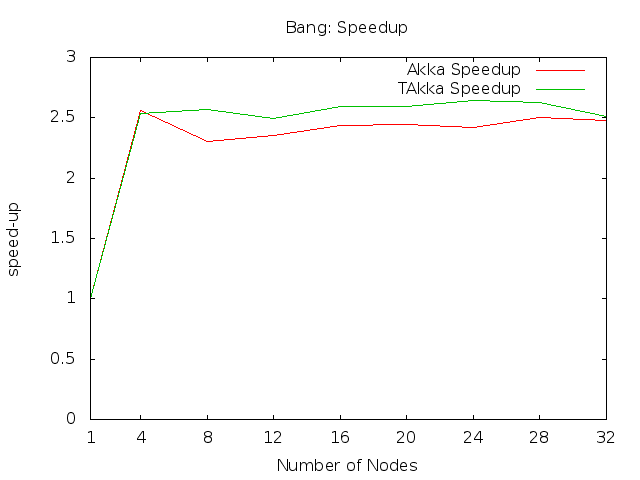
\includegraphics[scale=0.31]{efficiency/Bang_speedup.png}
        }\\
        \subfloat[Big Time]{
            \label{fig:1c}
            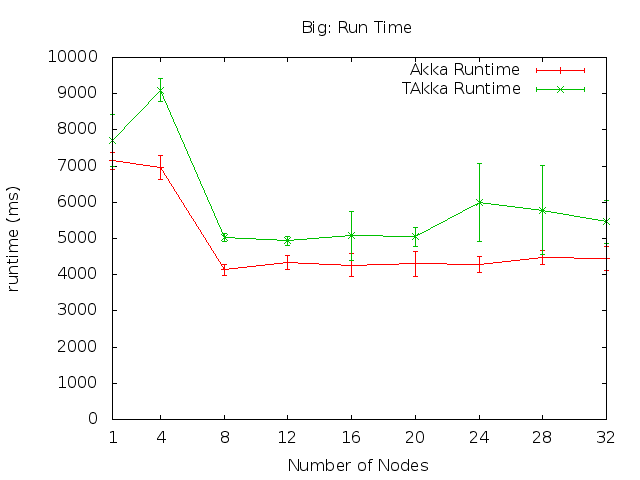
\includegraphics[scale=0.31]{efficiency/Big_time.png}
        }
        \subfloat[Big Scalability]{
           \label{fig:1d}
           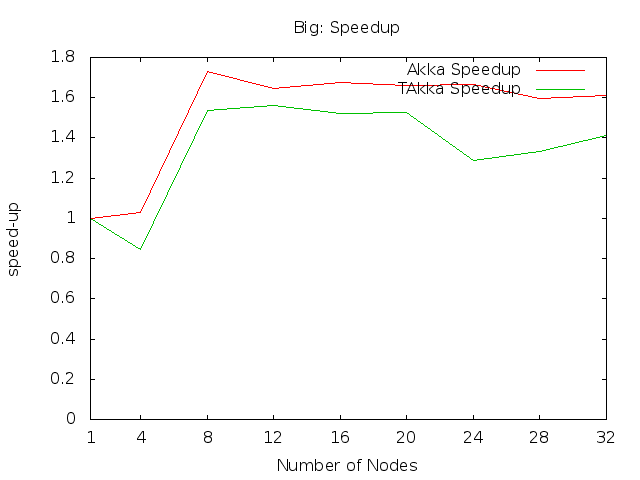
\includegraphics[scale=0.31]{efficiency/Big_speedup.png}
        }\\
        \subfloat[EHB Time]{
            \label{fig:1e}
            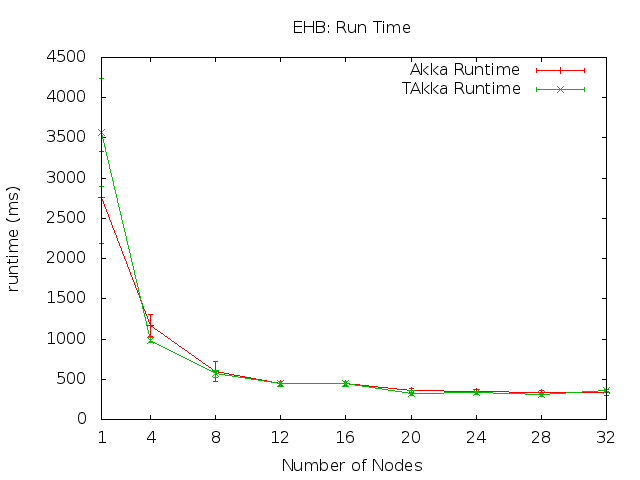
\includegraphics[scale=0.31]{efficiency/EHB_time.png}
        }
        \subfloat[EHB Scalability]{
           \label{fig:1f}
           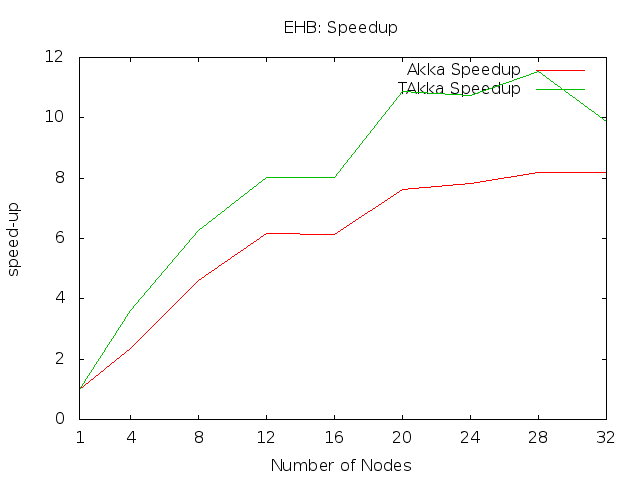
\includegraphics[scale=0.31]{efficiency/EHB_speedup.png}
        }\\
    \end{center}
    \caption{Runtime and Efficiency Benchmarks}
%   \label{runtime_efficiency}
\end{figure}
\begin{figure}[p]
    \ContinuedFloat
     \begin{center}
        \subfloat[GenStress Time]{
           \label{fig:1g}        
            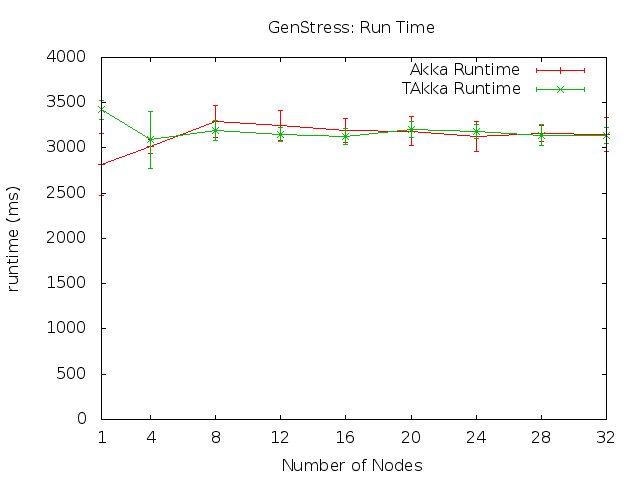
\includegraphics[scale=0.31]{efficiency/GenStress_time.png}
        }
        \subfloat[GenStress Scalability]{
           \label{fig:1h}
           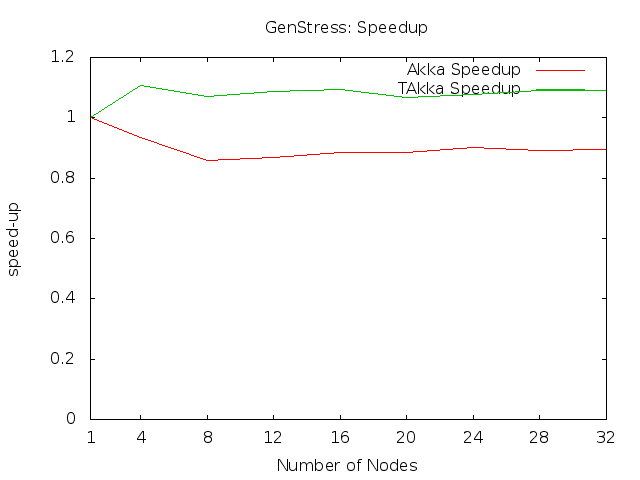
\includegraphics[scale=0.31]{efficiency/GenStress_speedup.png}
        }\\
        \subfloat[MBrot Time]{
            \label{fig:1i}
            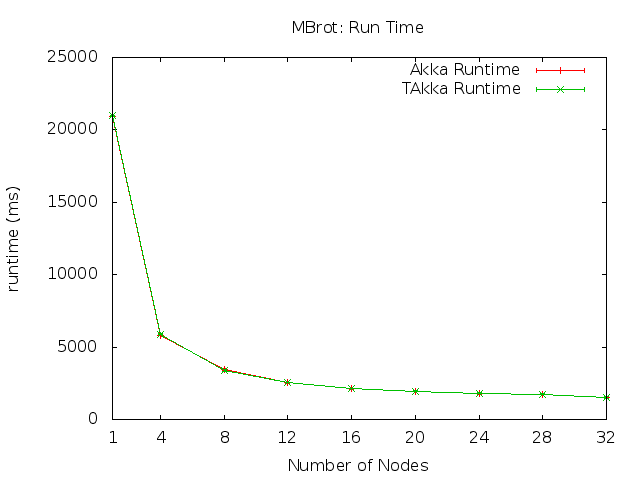
\includegraphics[scale=0.31]{efficiency/MBrot_time.png}
        }
        \subfloat[MBrot Scalability]{
           \label{fig:1j}
           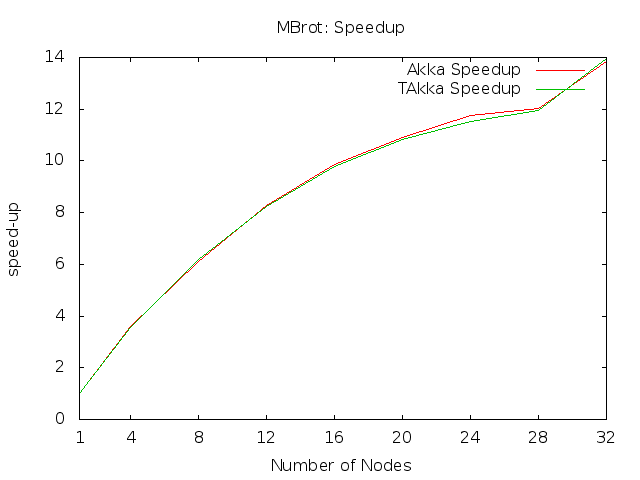
\includegraphics[scale=0.31]{efficiency/MBrot_speedup.png}
        }\\
        \subfloat[Parallel Time]{
            \label{fig:1k}
            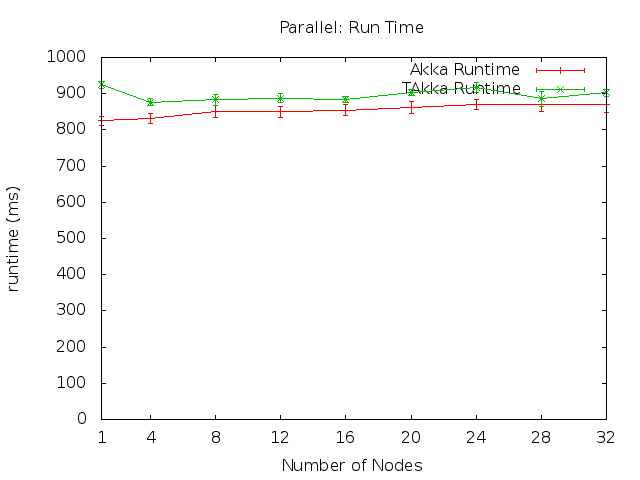
\includegraphics[scale=0.31]{efficiency/Parallel_time.png}
        }
        \subfloat[Parallel Scalability]{
           \label{fig:1l}
           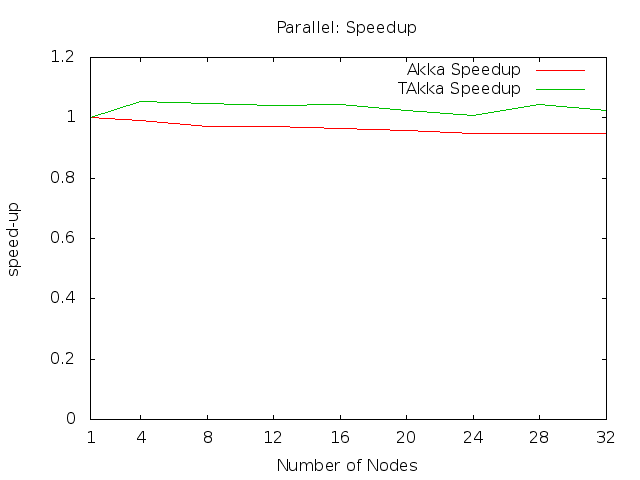
\includegraphics[scale=0.31]{efficiency/Parallel_speedup.png}
        }\\
    \end{center}
    \caption{Runtime and Efficiency Benchmarks}
%   \label{runtime_efficiency}
\end{figure}
\begin{figure}[p]
    \ContinuedFloat
     \begin{center}
        \subfloat[RAN Time]{
            \label{fig:1m}
            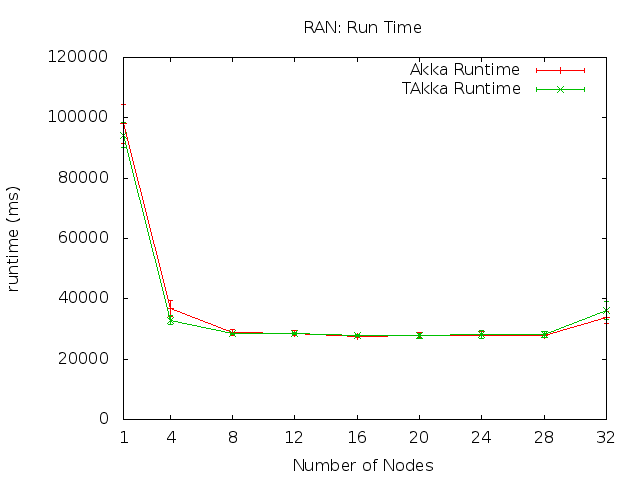
\includegraphics[scale=0.31]{efficiency/RAN_time.png}
        }
        \subfloat[RAN Scalability]{
           \label{fig:1n}
           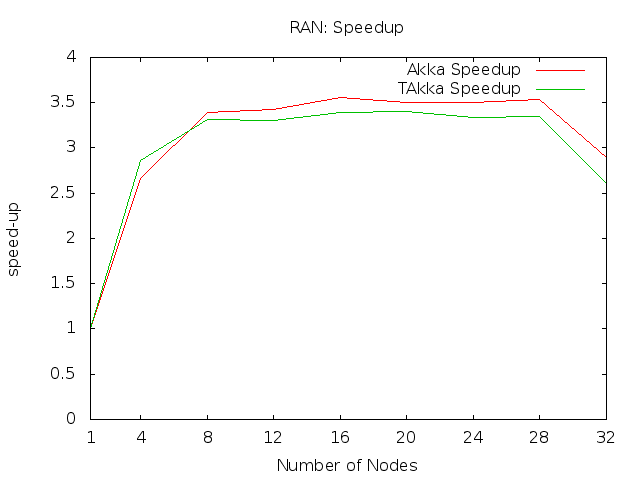
\includegraphics[scale=0.31]{efficiency/RAN_speedup.png}
        }\\
        \subfloat[SerialMsg Time]{
            \label{fig:1o}
            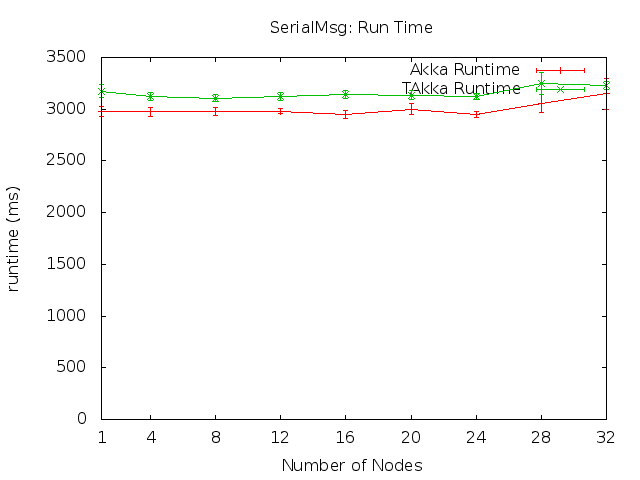
\includegraphics[scale=0.31]{efficiency/SerialMsg_time.png}
        }
        \subfloat[Serial Scalability]{
           \label{fig:1p}
           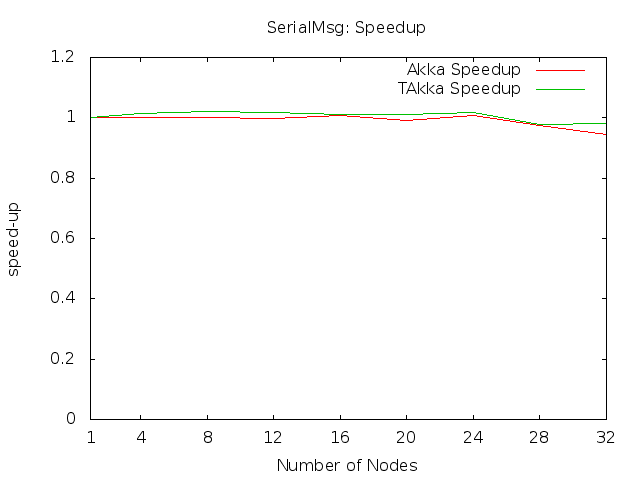
\includegraphics[scale=0.31]{efficiency/SerialMsg_speedup.png}
        }\\
    \end{center}
    \caption{Runtime and Efficiency Benchmarks}
   \label{runtime_efficiency}
\end{figure}


\newpage

\subsection{Additional Benchmarks}
\label{bench_fib}

\subsubsection{Fibonacci Numbers}

Results given in the last section show that the scalability of BenchErl 
examples varies.  Because BenchErl examples have similar structure and those 
examples are run on the same environment, the difference in their scalability 
may lie in differences in their computational tasks.  It is expected 
that the required runtime of a BenchErl example would depend on the time needed 
for completing the computation task and the time for assembling results.  
Because the master process is the only one that assembles the results, a 
BenchErl benchmark is $not$ likely to give a good scalability if most of its 
time is spent on collecting and processing the results of child processes.

To confirm that the scalability of a BenchErl benchmark depends on the ratio 
of the time spent on completing parallelized computational tasks and that spent 
on assembling results, a similar benchmark example was added, where each child 
process computes the {\it same} Fibonacci number {\it sequentially} using the following equation.

\begin{equation}
 f(n) = \begin{cases} 
            1,             & \mbox{if } n = 0 \ { or }\  n = 1  \\ 
            f(n-1)+f(n-2), & \mbox{if } n >=2
         \end{cases}
\end{equation}

The above basic way of computing a Fibonacci number was chosen because it has 
an exponential complexity to the input $n$, and hence the time to compute 
$f(n)$ changes dramatically when $n$ changes.

The parameters set in this example are the number of available nodes, the 
number of child processes, and the value of $n$ in $f(n)$.  The author expected 
that, when setting the number of child processes to a number higher 
than the number of available nodes, a benchmark with a higher $n$ would give 
better scalability than those with a lower $n$.  The above expectation
is confirmed by the benchmark result reported in Figure~\ref{fib_efficiency}.

\begin{figure}[p]
     \begin{center}
        \subfloat[Fib20 Time]{
            \label{fig:1q}
            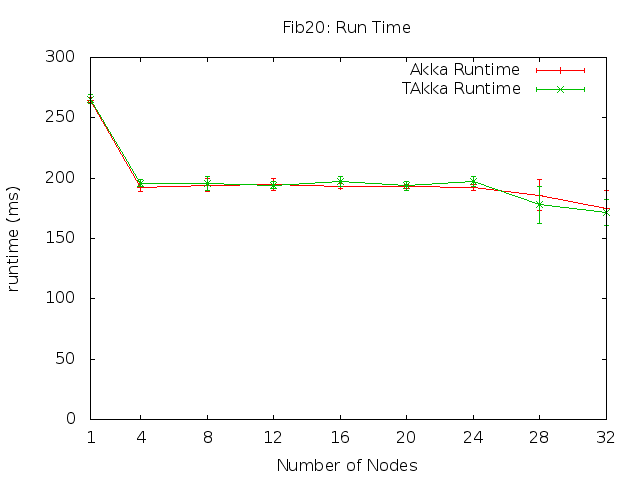
\includegraphics[scale=0.31]{efficiency/Fib20_time.png}
        }
        \subfloat[Fib20 Scalability]{
           \label{fig:1r}
           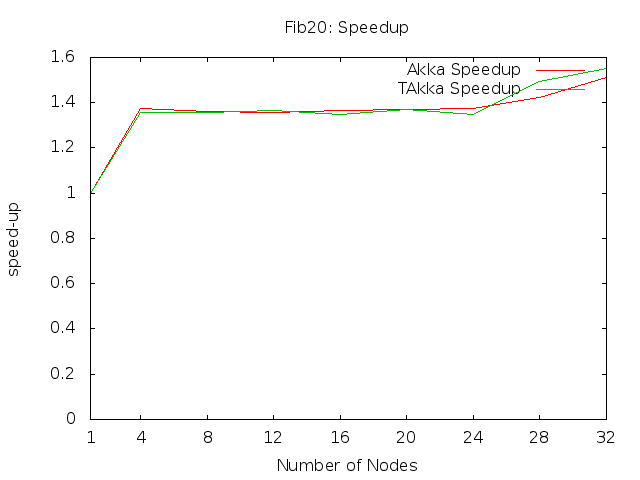
\includegraphics[scale=0.31]{efficiency/Fib20_speedup.png}
        }\\
        \subfloat[Fib30 Time]{
            \label{fig:1s}
            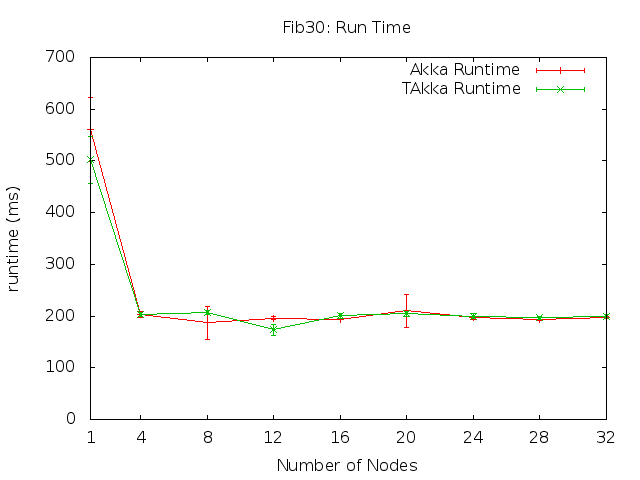
\includegraphics[scale=0.31]{efficiency/Fib30_time.png}
        }
        \subfloat[Fib30 Scalability]{
           \label{fig:1t}
           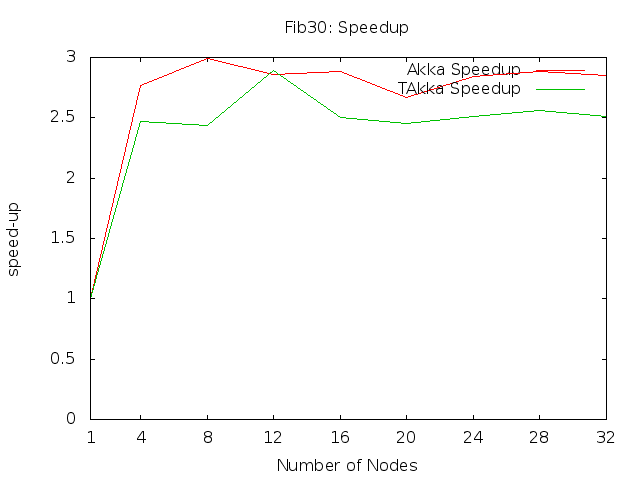
\includegraphics[scale=0.31]{efficiency/Fib30_speedup.png}
        }\\
        \subfloat[Fib40 Time]{
            \label{fig:1u}
            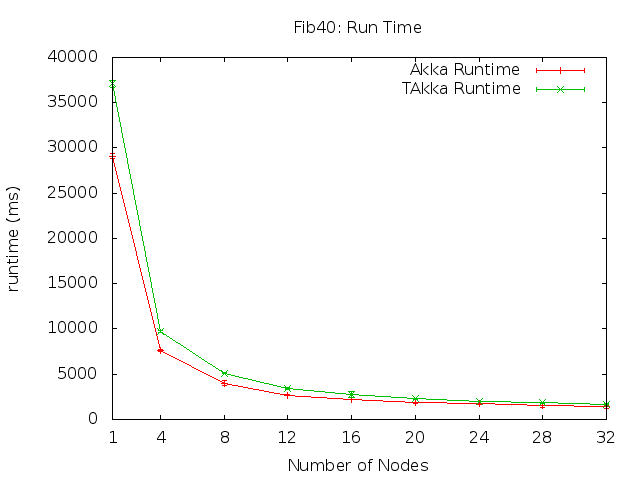
\includegraphics[scale=0.31]{efficiency/Fib40_time.png}
        }
        \subfloat[Fib40 Scalability]{
           \label{fig:1v}
           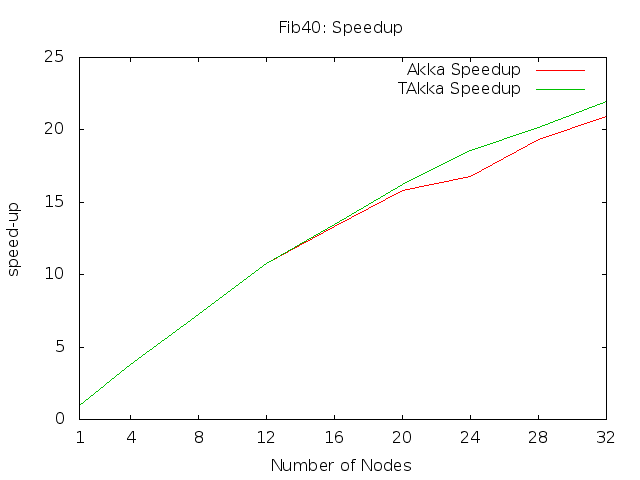
\includegraphics[scale=0.31]{efficiency/Fib40_speedup.png}
        }\\
    \end{center}
    \caption{Benchmark:Parallel Fibonacci Numbers}
   \label{fib_efficiency}
\end{figure}

\subsubsection{MBrot with different image sizes}

\begin{figure}[p]
     \begin{center}
        \subfloat[MBrot10 Time]{
            \label{fig:1q}
            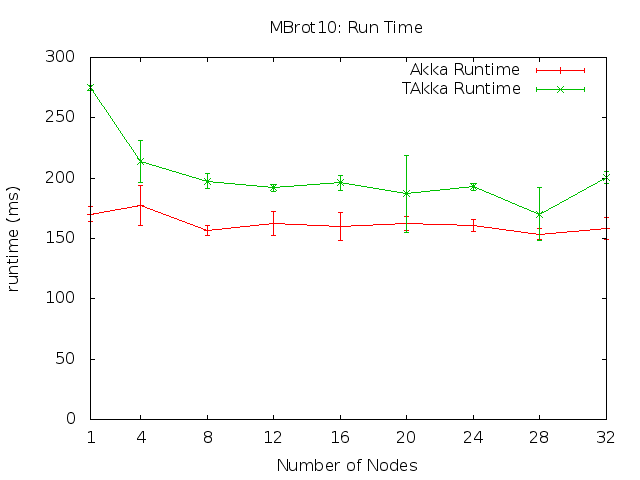
\includegraphics[scale=0.31]{efficiency/MBrot10_time.png}
        }
        \subfloat[MBrot10 Scalability]{
           \label{fig:1r}
           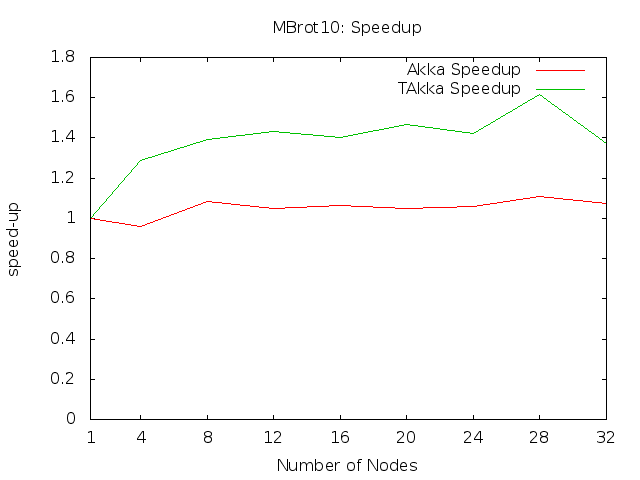
\includegraphics[scale=0.31]{efficiency/MBrot10_speedup.png}
        }\\
        \subfloat[MBrot1000 Time]{
            \label{fig:1s}
            \includegraphics[scale=0.31]{efficiency/MBrot1000_time.png}
        }
        \subfloat[MBrot1000 Scalability]{
           \label{fig:1t}
           \includegraphics[scale=0.31]{efficiency/MBrot1000_speedup.png}
        }\\
        \subfloat[MBrot6000 Time]{
            \label{fig:1u}
            \includegraphics[scale=0.31]{efficiency/MBrot_time.png}
        }
        \subfloat[MBrot6000 Scalability]{
           \label{fig:1v}
           \includegraphics[scale=0.31]{efficiency/MBrot_speedup.png}
        }\\
    \end{center}
    \caption{Benchmark: MBrot}
   \label{mbrot_efficiency}
\end{figure}

The result of the Fibonacci benchmark provides evidence that the scalability
of a distributed application can be bounded by the throughput of the master node.
The same conclusion is obtained when the image size of the MBrot example
is changed.   The MBrot example has a quadratic complexity 
to the image size.  In the BenchErl example, the image size is set to $6000$ 
pixels $ \times$  $ 6000$ pixels so that more time is spent on computation than 
message sending.  Figure~\ref{mbrot_efficiency} reports the results when the 
image size is set to $10$ pixels $ \times$  $ 10$ pixels, $1000$ pixels $ 
\times$  $ 1000$ pixels, and $6000$ pixels $ \times$  $ 6000$ pixels.   As 
expected, the result is similar to the result of the Fibonacci benchmark.  
% The highest speed-up achieved in the MBrot example is smaller than the one in the
% Fibonacci example because each child node in the MBrot example has less computational
% cost.

\subsubsection{The N-Queens Problem}

In the BenchErl examples and the Fibonacci example, child processes are asked to 
execute the same computation a number of times (Section~\ref{bencherl_overview}).  In contrast, distributed and 
cluster computing techniques are often used to solve a computationally 
expensive task by distributing sub-tasks to independent nodes.  To simulate 
such a scenario, another benchmark, N-Queens Puzzle, is added. 

The N-Queen Puzzle \citep{wiki:nqueens} looks for {\it all} solutions of 
placing $n$ queens on an $n \times n$ chessboard such that no two queens share 
the same row, column, or diagonal.  In the benchmark, a master node first uses 
a width-first backtracking algorithm to expand the search space.  If the 
number of candidate partial solutions is greater than twice the available 
nodes, the master node sends partial solutions to those nodes which use a 
depth-first backtracking algorithm to find all possible solutions of each 
candidate partial solution. In this example, two solutions are considered 
distinct if they differ only in symmetry operations.

Finding all solutions of an N-Queen Puzzle is an NP-hard problem.  Therefore, a 
suitable $n$ makes the problem a good benchmark to demonstrate the advantage of 
cluster and distributed programming.  Figure~\ref{nqueens_efficiency}
reports the result when $n$ is set to $14$.  The value of $n$ is chosen 
according to the same criteria for BenchErl benchmarks as stated in Section 
\ref{bench_parameters}.  The result shows that both the Akka and 
TAkka implementation have good scalability and similar efficiency.


\begin{figure}[h]
     \begin{center}
        \subfloat[N-Queens Time]{
            \label{fig:1q}
            \includegraphics[scale=0.3]{efficiency/NQueens_time.png}
        }
        \subfloat[N-Queens Scalability]{
           \label{fig:1r}
           \includegraphics[scale=0.3]{efficiency/NQueens_speedup.png}
        }
    \end{center}
    \caption{Benchmark: N-Queens Puzzle}
   \label{nqueens_efficiency}
\end{figure}



\newpage
\section{Assessing System Reliability and Availability}
\label{reliability}

The supervision tree principle is adopted by Erlang and Akka users in the 
hope of improving the reliability of software applications.  Apart from the 
reported nine "9"s reliability of Ericsson AXD 301 switches 
\citep{ArmstrongAXD} and the wide range of Akka use cases, how could software 
developers assure the reliability of their newly implemented applications?  

TAkka is shipped with a Chaos Monkey library and a Supervision View library for 
assessing the reliability of TAkka applications.  A Chaos Monkey test randomly 
kills actors in a supervision tree and a Supervision View test dynamically 
captures the structure of supervision trees.  With the help of Chaos Monkey and 
Supervision View, users can visualize how their TAkka applications react to 
adverse conditions. Missing nodes in the supervision tree (Section 
\ref{calculator_chaos_test}) show that failures occur during the test. On the 
other hand, any failed actors are restored, and hence appropriately supervised 
applications (Section~\ref{bencherl_chaos_test})  pass Chaos Monkey tests.



\subsection {Chaos Monkey and Supervision View}

Chaos Monkey \citep{ChaosMonkey} randomly kills Amazon Elastic Compute Cloud 
(Amazon EC2) instances in an Auto Scaling Group.  In a Chaos Monkey test, the 
reliability of an application is tested against intensive adverse 
conditions.  The same idea is ported into Erlang to detect potential flaws of 
supervision trees \citep{ErlangChaosMonkey}.  The TAkka library ports the 
Erlang version of Chaos Monkey.  In addition to randomly killing actors, 
users can simulate other common failures by using the following modes.

\paragraph{Random} This is the default mode of Chaos Monkey.  It randomly
choose one of the other modes in each run.

\paragraph{Exception} This mode simulates the case that an exception is raised
from an actor.  The randomly picked victim actor raises an exception from a
user-defined set of exceptions.


\paragraph{Kill} This mode simulates the case that a recoverable failure is occurred
inside an actor.  A {\tt Kill} message is sent to a randomly picked victim actor to see
if it can be restarted by its supervisor.

\paragraph{PoisonKill} This mode simulates that case that an unidentifiable failure
is occurred inside an actor.  A {\tt PoisonKill} message is sent to a randomly
picked victim actor.  The actor is terminated permanently and cannot be restarted
by its supervisor.  It tests whether the application has other failure recovery
mechanism for that actor.  Being supervised is sufficient for most actors.  However,
for some critical actors, having additional assurance might be required in practice.

\paragraph{NonTerminate} This mode simulates network congestion or a design flow of
actor implementation.  A randomly picked actor runs into an infinite loop and
consumes system resources but cannot process any messages.  A robust system should be
able to detect such flow or network congestion, redirect further messages to a new
actor, and try to kill the problematic actor.

\begin{comment}

\begin{table}[h]
\begin{center}
\begin{tabular}{| c | p{4.6 cm} | p{5.2 cm} | }
\hline
Mode & Failure & Description \\
\hline
Random (Default) & Random Failures & Randomly choose one of the other modes in 
each run. \\
\hline
Exception & Raise an exception & A victim actor randomly raise an exception 
from 
a user-defined set of exceptions. \\
\hline
Kill & Failures that can be recovered by scheduling service restart &  
Terminate 
a victim actor.  The victim actor can be restarted later. \\
\hline
PoisonKill & Unidentifiable failures & Permanently terminate a victim actor.  
The victim cannot be restarted.  \\ 
\hline 
NonTerminate & Design flaw or network congestion & Let a victim actor run 
into an infinite loop.  The victim actor consumes system resources but cannot 
process any messages. \\
\hline

\end{tabular}
\caption{TAkka Chaos Monkey Modes}
\label{chaos}
\end{center}
\end{table}

\end{comment}

Figure~\ref{chaos_api} gives the API and the core implementation of TAkka Chaos 
Monkey.  A user sets up a Chaos Monkey test by initializing a 
{\tt ChaosMonkey} instance, defining the test mode, and scheduling the interval 
between each run.  In each run, the {\tt ChaosMonkey} instance sends a 
randomly picked actor a special message.  Upon receiving a Chaos Monkey 
message, a TAkka actor executes a piece of problematic code as described above.  
{\tt PoisonPill} and {\tt Kill} are handled by {\tt 
systemMessageHandler} and can be overridden (Figure~\ref{takka_actor_api}).  
{\tt ChaosException} and {\tt ChaosNonTerminate}, on the 
other hand, are handled by the TAkka library and cannot be overridden.

\begin{figure}[p]

\begin{lstlisting}
package takka.chaos
class ChaosMonkey(victims:List[ActorRef[_]], exceptions:List[Exception]){
  private var status:Status = OFF;
  def setMode(mode:ChaosMode);
  def enableDebug();
  def disableDebug();
  def start(interval:FiniteDuration)  = status match {
    case ON => 
throw new Exception("ChaosMonkey is running: turn it off before restart it.") 
    case OFF =>
      status = ON
      scala.concurrent.future {
        repeat(interval)
      }
  }
  def turnOff()= {status = OFF}
  private def once() {
    var tempMode = mode
    if (tempMode == Random){
      tempMode = Random.shuffle(
                 ChaosMode.values.-(Random).toList).head
    }
    val victim = scala.util.Random.shuffle(victims).head
    tempMode match {
      case PoisonKill =>
        victim.untypedRef ! akka.actor.PoisonPill
      case Kill =>
        victim.untypedRef ! akka.actor.Kill
      case Exception =>
        val e = scala.util.Random.shuffle(exceptions).head
        victim.untypedRef ! ChaosException(e)
      case NonTerminate =>
        victim.untypedRef ! ChaosNonTerminate   
  } }
  private def repeat(period:FiniteDuration):Unit =  status match {
    case ON =>
      once
      Thread.sleep(period.toMillis)
      repeat(period)      
    case OFF =>
} } 
object ChaosMode extends Enumeration {
    type ChaosMode = Value
    val Random, PoisonKill, Kill, Exception, NonTerminate  = Value
}
\end{lstlisting}
\caption{TAkka Chaos Monkey}
\label{chaos_api}
\end{figure}


\subsection{Supervision View}


To dynamically monitor changes in supervision trees, the author designed and 
implemented a Supervision View library. In a supervision view test, an instance 
of {\tt ViewMaster} periodically sends request messages to interested actors.  
When the request message is received, an active TAkka actor replies its 
status to the {\tt ViewMaster} instance and passes the request message to its 
children.  The status message includes its actor path, paths of its children, 
and the time when the reply is sent.  The {\tt ViewMaster} instance records 
status messages and passes them to a visualizer, which will analyze and 
interpret changes in the tree structure during the testing period.


A view master is initialized by calling one of the apply methods of the {\tt 
ViewMaster} object as given in Figure~\ref{supervision_view}.
Each view master has an actor system and a master actor as its fields.  The 
actor system is set up according to the given {\tt name} and {\tt config}, or 
the default configuration.  The master actor, created in the actor system, has 
type {\tt Actor[SupervisionViewMessage]}.  After the start method of a 
view master is called, the view master periodically sends {\tt 
SupervisionViewRequest} to interested nodes in supervision trees, where 
{\tt date} is the system time just before the view master sends requests.  
When a TAkka actor receives {\tt SupervisionViewRequest} message, it sends a 
{\tt SupervisionViewResponse} message back to the view master and passes the \\ 
{\tt SupervisionViewRequest} message to its children.  The {\tt date} value
in a \\ {\tt SupervisionViewResponse} message is the same as the {\tt date} 
value 
in the corresponding {\tt SupervisionViewRequest} message.  Finally, the master 
actor of the view master records all replies in a hash map from {\tt Date} to 
{\tt TreeSet[NodeRecord]}, and sends the record to an appropriate drawer on 
request. 



\begin{figure}[!h]

\begin{lstlisting}
package takka.supervisionview
sealed trait SupervisionViewMessage
case class SupervisionViewResponse(date:Date, reportorPath:ActorPath, 
    childrenPath:List[ActorPath]) extends SupervisionViewMessage
case class ReportViewTo
    (drawer:ActorRef[Map[Date, TreeSet[NodeRecord]]]) 
    extends SupervisionViewMessage

case class SupervisionViewRequest(date:Date,  
              master:ActorRef[SupervisionViewResponse])
case class NodeRecord(receiveTime:Date, node:ActorPath, 
              childrenPath:List[ActorPath]) 

object ViewMaster{
  def apply(name:String, config: Config, topnodes:List[ActorRef[_]], 
              interval:FiniteDuration):ViewMaster
  
  def apply(name:String, topnodes:List[ActorRef[_]], 
              interval:FiniteDuration):ViewMaster
  
  def apply(topnodes:List[ActorRef[_]], 
              interval:FiniteDuration):ViewMaster
}


\end{lstlisting}
\caption{Supervision View}
\label{supervision_view}
\end{figure}

\begin{figure}[p]
     \begin{center}
        \subfloat[]{
            \label{fig:tree1}
            \includegraphics[scale=0.6]{Tree1.png}
        }\\
        \subfloat[]{
           \label{fig:tree2}
           \includegraphics[scale=0.6]{Tree2.png}
        }\\
        \subfloat[]{
            \label{fig:tree3}
            \includegraphics[scale=0.6]{Tree3.png}
        }
    \end{center}
    \caption{Supervision View Example}
   \label{fig:supervisionview}
\end{figure}

\subsection{A Partly Failed Safe Calculator}
\label{calculator_chaos_test}

In the hope that Chaos Monkey and Supervision View tests could reveal 
the breaking points in a supervision tree, the author modified the Safe 
Calculator example and ran a test as follows.  Firstly, three 
safe calculators were run on three Beowulf nodes, under the supervision of a 
root actor using the {\tt OneForOne} strategy with {\tt Restart} action.  
Secondly, different supervisor strategies were set for each safe calculator.  
The first safe calculator, S1, restarts any failed child immediately.  This 
configuration simulates a quick restart process. The second safe calculator, 
S2, computes a Fibonacci number in a naive way for about 10 seconds before 
restarting any failed child.  This configuration simulates 
a restart process which may take a noticeable time.  The third safe calculator, 
S3, stops the child when it fails.  Finally, a Supervision View test was set to 
capture the supervision tree every 15 seconds, and a Chaos Monkey 
test was set to kill a random child calculator every 3 seconds.

A test result, given in Figure~\ref{fig:supervisionview}, gives the expected
tree structure at the beginning, 15 seconds and 30 seconds of the test.  Figure 
\ref{fig:tree1} shows that the application initialized three safe calculators 
as described.  In Figure~\ref{fig:tree2}, S2 and its child are marked as dashed 
circles because it takes the view master more than 5 seconds to receive their 
responses.  From the test result itself, a user cannot tell whether the delay 
is due to a blocked calculation or network congestion.  Comparing against 
Figure~\ref{fig:tree1}, the child of S3 is not shown in Figure~\ref{fig:tree2} 
and Figure~\ref{fig:tree3} because no response is received from it until the 
end of the test.  When the test ends, no response to the last request is 
received from S2 and its child.  Therefore, both S2 and its child are not shown 
in Figure~\ref{fig:tree3}.  S1 and its child appear in all three Figures 
because either they never fail during the test or they are recovered from 
failures within a short time.




\subsection{BenchErl Examples with Different Supervisor Strategies}
\label{bencherl_chaos_test}

To test the behaviour of applications with internal states under 
different supervisor strategies, the author applied the {\tt OneForOne} 
supervisor strategy with different {\tt Directive}s (Figure~\ref{takka_supervisor_strategy}) to the 8 BenchErl examples 
and tested them using Chaos Monkey and Supervision View.  The master node of 
each BenchErl test was initialized with an internal counter.  The internal 
counter decreased when the master node received finishing messages from its 
children.  The test application stopped when the internal counter of the master 
node reached 0.  The Chaos Monkey test is set with the {\tt Kill} mode 
and randomly killed a victim actor every second.  When the {\tt Escalate} 
directive is applied to the master node, the test stops as soon as the first {\tt 
Kill} message is sent from the Chaos Monkey test.  When the {\tt Stop} directive 
is applied, the application does not stop and, eventually, the supervision view 
test only receives messages from the master node.  When the {\tt Restart} 
directive is applied, the application does not stop but the Supervision View test 
receives messages from the master node and its children.  When the {\tt Resume} 
directive is applied, all tests stop eventually with a longer run-time compared to 
tests without Chaos Monkey and Supervision View.



\begin{comment}
\subsubsection{Limitation of Accelerated Software Reliability Test}

By following the Supervision Principle, software developers hope their 
applications can be tolerant of run-time exceptions.
\end{comment}

\section{Summing Up}

This chapter confirms that TAkka can detect type errors without bringing in 
obvious overheads.  Firstly, all small and medium sized Akka examples used in 
this chapter are straightforwardly rewritten using the TAkka library, by 
updating about 7.4\% of the source code.  Through the porting process, a type 
error was found in the Socko framework.  The case study in Section 
\ref{takka_evaluation} shows that TAkka has the 
advantage of solving the type pollution problem.  Secondly, web 
servers built using Akka and TAkka reach similar throughput when the same 
number of EC2 instances are used.  Thirdly, BenchErl benchmark examples written 
in Akka and TAkka have similar efficiency and scalability when running on a 
32 node Beowulf cluster.  The additional benchmark examples in Section 
\ref{bench_fib} provide evidences that the scalability of an application 
depends on the ratio of the cost of parallelized computational tasks and the 
cost of throughput bounded communications.  Lastly, TAkka provides a ChaosMonkey 
library and a Supervision View library for assessing the correctness of 
applications built using TAkka. 



 \chapter{Summary and Future Work}
\label{summary}

The main goal of this thesis is the development of a library that combines the 
advantages of type checking and the supervision principle.  The aim is to 
contribute to the construction of reliable distributed applications using 
type-parameterized actors and supervision trees.  Aside from the TAkka library 
itself, this thesis has presented the evaluation results of TAkka.  The 
evaluation metrics in this thesis can be used and further developed for the 
evaluation of other libraries that implement actors and supervision trees.  This 
chapter reviews the research results presented in the thesis, suggests future 
research topics, and concludes.


\section{Overview of Contributions}


\subsection{A library for Type-parameterized Actors and Their Supervision}

The key contribution of this thesis is the design and implementation of the 
TAkka library, which is the first programming library where type parameterized 
actors can form a supervision tree.  The TAkka library is built on top of Akka, 
a library which has been used for implementing real world applications.  The 
TAkka library adds type checking features to the Akka library but
delegates tasks such as actor creation and message passing to the underlying
Akka systems. 

The TAkka library uses both static and dynamic type checking so that type 
errors are detected at the earliest opportunity. To enable look up on remote 
actor references, TAkka defines a typed name server that keeps maps from typed 
symbols to values of the corresponding types.

In addition, Akka  programs can gradually migrate to their TAkka equivalents 
(evolution) rather than require providing type parameters everywhere 
(revolution).  The above property is analogous to adding generics to Java 
programs.

Compared with Akka, the TAkka library avoids the type pollution 
problem straightforwardly.  The type pollution problem, discussed in 
Section~\ref{type_pollution}, refers to the situation where a user can send a 
service message not expected from him or her because that service publishes too 
much type information about its communication interface. Without due care, 
the type pollution problem may occur in actor-based systems that are 
constructed using the layered architecture \citep{DijkstraTHE, 
buschmann2007pattern} or the MVC pattern \citep{reenskaug1979original, 
reenskaug2003model}, two popular design patterns for constructing modern 
applications.  A demonstration example shows that avoiding the type 
pollution problem in TAkka is as simple as publishing a service as having 
different types when it is used by different parties.

\subsection{A Library Evaluation Framework}

The second contribution of this thesis is a framework for evaluating the 
TAkka library.  The author believes that the employed evaluation metrics can be 
used and further developed for evaluating other libraries that implement actors 
and the supervision principle.

By porting existing small and medium sized Erlang and Akka applications, 
results in Section~\ref{expressiveness} and \ref{efficiency} show that 
rewriting Akka programs using TAkka will {\it not} bring obvious runtime and 
code-size overheads. As regards expressiveness, {\it all} Akka applications 
considered in this thesis can be ported to their TAkka equivalents with a small 
portion of code modifications.  The TAkka library is expected to have the {\it 
same} expressiveness as the Akka library.

Finally, the reliability of a TAkka application can be partly assessed by using
the Chaos Monkey library and the Supervision View library.  
The Chaos Monkey library, ported from the work by \citet{ChaosMonkey} and 
\citet{ErlangChaosMonkey}, tests whether an application can survive in an 
adverse environment where exceptions raise randomly.  The Supervision View 
library dynamically captures the structure of supervision trees.  With the help 
of the Chaos Monkey library and the Supervision View library, application 
developers can visualise how the application will behave under the tested 
condition.

\section{Future Work}
\label{future_work}

The work presented in this thesis confirms that actors in supervision trees can
be typed by parameterising the actor class with the type of messages it expects
to receive. The results of primary evaluations show that the TAkka library 
can prevent some errors without bringing obvious overheads compared with 
equivalent Akka applications. As actors and supervision trees are widely used 
in the development of distributed applications nowadays, the author believes 
that there is great potential for the TAkka library. Much more can be done to 
make TAkka more usable, as well as to further the goal of making the building 
of reliable distributed applications easier.


\subsection{Supervision and Typed Actor in Other Systems}

The result of this thesis confirms the feasibility of using type parameterized 
actors in a supervision tree.  The resulting TAkka library is built on top of 
Akka for the following three considerations:  Firstly, both actor and 
supervision have been implemented in Akka.  The legacy work done by the Akka 
developers makes it possible for us to focus on the core research question. 
That is, to what extent can actors in a supervision tree be statically typed?  
Secondly, Akka is 
built in Scala, a language that has a flexible type system.  The flexibility 
provided by Scala allows the author to explore types in a supervision tree.  In 
TAkka, dynamic type checking is only used when static type checking meets its 
limitations. Thirdly, Akka is a popular programming framework.  As part of the 
Typesafe stack, Akka has been used for developing applications in different 
sizes and for different purposes.  If Akka applications can be gradually 
upgraded to TAkka applications, the author believes that the type checking 
feature in TAkka can improve the reliability of existing Akka systems.

Actor programming has been ported to many languages.  The notion of type 
parameterized actors, however, was introduced very recently in libraries such 
as Cloud Haskell \citep{CloudHaskell} and scalaz \citep{scalaz}.  It has been 
proposed to implement a supervision tree in Cloud Haskell 
\citep{OTPCloudHaskell}.  The author believes that the techniques used in this 
thesis can help the design of the future versions of Cloud Haskell.



\subsection{Benchmark Results from Large Real Applications}

This thesis compares TAkka with Akka with regards to several dimensions by 
porting small and medium sized applications. Most of selected examples are 
from open source projects. The author gratefully acknowledges the RELEASE team 
for giving us access to the source code of the BenchErl benchmark examplesl; 
Thomas Arts from QuviQ.com and Francesco Cesarini from Erlang Solutions for 
providing the Erlang source code for the ATM simulator example and the Elevator 
Controller example, both of which are used in their commercial training 
courses. Nevertheless, experiments on large real applications are not 
considered due to the restriction of time and other required 
resources. It would be interesting to know whether TAkka can help the 
construction and reliability of large commercial or research applications.



\subsection{Supervision Tree that Supports Software Rejuvenation}

The core idea of the Supervision Principle is to restart components {\it 
reactively} when they fail. Similarly, software rejuvenation 
\citep{huang1995software, dohi2000statistical} is a  {\it preventive} failure 
recovery mechanism which periodically restarts components with a clean internal 
state. The interval of restarting a component, called  {\it software 
rejuvenate schedule}, is set to a fixed period. Software rejuvenation has been 
implemented in a number of commercial and scientific applications to improve 
their longevity. As a supervisor can restart its children, can  {\it software 
rejuvenate schedule} be set for each actor?

\subsection{Measuring and Predicting System Reliability}

Due to the nature of software development, the library itself cannot guarantee 
the reliability of applications built using it; nor can the achieved 
high reliability of Erlang applications indicate that a newly 
implemented application using the supervision principle will have desired 
reliability.   To help software developers identify bugs in their applications, 
the ChaosMonkey library and the SupervisionView library are shipped with TAkka. 
 However, a quantitative measurement of software reliability under operational 
environment is still desired in practice.  To solve this problem, two 
approaches are discussed following.

The first approach is measuring the target system as a black-box.  
Unfortunately, \citet{Littlewood93} show that even long term failure-free 
observation itself does not mean that the software system will achieve high 
reliability in the future.  

The second approach is giving a specification of actor-based supervision tree 
and measuring the reliability of a supervision tree as the accumulated result 
of reliabilities of its sub-trees. 
By eliminating language features that are not related to supervision, both the worker 
node and the supervisor node in a supervision tree can be modelled as  
Deterministic Finite Automata.  Analysis shows that various
supervision trees can be modelled by a supervision tree that only contains 
simple worker nodes and simple supervisor nodes. 
To accomplish this study, the following problems need to be solved:
\begin{itemize}
  \item What are possible dependencies between nodes? For each dependency,
what is the algebraic relationship between the reliability of a sub-tree
and reliabilities of individual nodes?
  \item Based on the above result, how are the overall reliabilities
of a supervision tree to be calculated? When will the reliability be improved 
by using a supervising tree, and when will it not be?
  \item Given the reliabilities of individual workers and constraints between
them, is there an algorithm to give a supervision tree with desired 
reliability?  If not, can we determine if the desired reliability is not
achievable?
\end{itemize}

\section{Conclusion}

The author believes that the demand for distributed applications will continue 
increasing in the next few years.  The recent trends of emphasis on programming 
for the cloud and mobile platforms all contribute to this direction.  With the 
growing demands and complexity of distributed applications, their reliability 
will be one of the top concerns among application developers. 

The TAkka library introduces a type-parameter for actor-related classes. The 
additional type-parameter of a TAkka actor specifies the communication 
interface of that actor.  The author is glad to see that type-parameterized 
actors can form supervision trees in the same way as untyped actors.
Lastly, test results show that building type-parameterized actors on top of 
Akka does not introduce significant overheads, with respect to program size,
efficiency, and scalability.  In addition, debugging techniques such 
as Chaos Monkey and Supervision View can be applied to applications built 
using actors with supervision trees.  The above results encourage the use of 
types and supervision trees to implement reliable applications and improve the 
reliability of legacy applications with little effort.  The author expects 
similar results can be obtained in other actor libraries.






% \begin{comment}
\chapter{Reliability: Statistic Background}
\end{comment}

% \begin{comment}
 


\chapter{Reliability of Supervision Tree}


\section{Single Node Analysis}

Case 0: Single Failure, No restart
\begin{equation}
R(t) = \int_{t}^{\infty} f(x)dx
\end{equation}
\begin{equation}
A(t) = \frac{\int_{0}^{t} xf(x)dx + t \cdot R(t) }{t}  
\end{equation}
Case I: Every $T$ time, spend $t_R$ time to restart

\begin{equation}
A(t) = \frac{ n(\int_{0}^{T} x f(x) dx + T \cdot R(T)) + \int_{0}^{t_{tail}} x 
f(x) dx}{t}
\end{equation}
\hspace{7 cm} where  $n = \left \lfloor \frac{t}{T+t_R} \right \rfloor$ and 
$t_{tail} = t-nT$


Case II: When failed, spend $t_R$ time to restart

\begin{equation}
A(t) = ?
\end{equation}

\hspace{7 cm} where  $W(t) = \int_{0}^{t} xf(x)dx$

Case III: When failed or running for $T$ time, spend $t_R$ time to restart


$A(t) = ? $

\end{comment}

% \chapter{A Precise Model for Software Rejuvenation}
\label{rejuvenation_model}




\bibliographystyle{apalike}
\bibliography{Jiansen}

% \appendix
%  \section{Examples for Expressiveness and Correctness Test}
\label{app_correct}

\begin{description}
  \item[ATM simulator\cite{quviq} ] A bank ATM simulator with backend database
and frontend GUI.
  \item[Elevator Controller \cite{quviq}] A system that monitors and schedules a
number of elevators. 
  \item[Ping Pong \cite{akka_doc} ] A simple message passing application.
  \item[Dining Philosophers \cite{akka_doc}] A application that simulates the
dining philosophers problem using Finite State Machine (FSM) model.
  \item[Distributed Calculator \cite{akka_doc}] An application that examines
distributed computation and hot code swap.
  \item[Fault Tolerance \cite{akka_doc}] An application that demonstrates how
system responses to component failures.
  \item[Barber Shop\cite{BarberShop} ] A application that simulates the Barber
Shop problem. 
  \item[EnMAS \cite{EnMAS}] An environment and simulation framework for
multi-agent and team-based artificial intelligence research

  \item[Socko Web Server \cite{SOCKO} ]  lightweight Scala web server that can
serve static files and support RESTful APIs
  \item[Gatling \cite{Gatling}] A stress testing tool.
\end{description}


\section{Examples for Efficiency and Scalability Test}

\begin{description}
  \item [bang] This benchmark tests many-to-one message passing.  The benchmark
spawns a specified number sender and one receiver.  Each sender sends a
specified number of messages to the receiver.
  \item [big] This benchmark tests many-to-many message passing.  The benchmark
creates a number of actors that exchange ping and pong messages.
  \item [ehb] This is a benchmark and stress test.  The benchmark is
parameterized by the number of groups and the number of messages sent from each
sender to each receiver in the same group.
  \item [mbrot] This benchmark models pixels in a 2-D image.  For each pixel,
the benchmark calculates whether the point belongs to the Mandelbrot set.
  \item [parallel] This benchmark spawns a number of processes, where a list of
N timestamps is concurrently created.
  \item [genstress] This benchmark is similar to the bang test.  It spawns an
echo server and a number of clients.  Each client sends some dummy messages to
the server and waits for its response.  The Erlang version of this test can be
executed with or without using the gen\_server behaviour.  For generality, this
benchmark only tests the version without using gen\_server.
  \item [serialmsg] This benchmark tests message forwarding through a
dispatcher.
  \item [timer\_wheel] This benchmark is a modification to the big test.  While
responding to ping messages, a process in this message also waits pong messages.
 If no pong message is received within the specified timeout, the process
terminates itself.
  \item [ran] This benchmark spawns a number of processes.  Each process
generates a list of ten thousand random integers, sorts the list and sends the
first half of the result list to the parent process.
\end{description}
% \addcontentsline{toc}{chapter}{APPENDICES}

% \chapter{Artefacts}

Artefacts produced during this projects are saved in the following repositories.

\section{Project Private Repository}

URL: https://svn.ecdf.ed.ac.uk/repo/user/s1024484/

This svn repository includes 


\begin{itemize}
  \item annual reports from 2010/2011 to 2012/2013
  \item a copy of the TAkka repository, with the source code of Erlang, Akka, 
and TAkka implementations of the the ATM example \citep{atmprivate} and the 
elevator controller example \citep{quviq}.
  \item a copy of the TAkka Play Repository.
  \item a copy of the FreeBench Repository.
%  \item a copy of the Rejuvenation Repository.
  \item an extension of the Links programming language that supports 
join-patterns (reference).
  \item a copy of this thesis and a [paper] summaries this project.
\end{itemize}


\section{TAkka Public repository}

URL: https://github.com/Jiansen/TAkka

This github repository includes the source code of the TAkka library, testing 
examples and instructions of using the code.  The ATM example \citep{atmprivate} 
and the elevator controller example \citep{quviq} are not included in this 
public repository for copyright reasons.  The TAkka implementation for the Play 
framework is in a separate repository.

\section{TAkka Play}
URL: https://github.com/Jiansen/TAkka-Play

This github repository includes the source code of the TAkka 
implementation of the Play framework.


\section{FreeBench Repository}
URL: https://github.com/Jiansen/FreeBench

This github repository includes the source code of the FreeBench tool, 
described in Section \ref{throughput}.


\begin{comment}
\section{Rejuvenation Repository}

URL: https://github.com/Jiansen/Rejuvenation


This github repository includes the source code of the TAkka library, testing 
examples except the ATM example \citep{atmprivate} and the elevator controller 
example \citep{quviq}, and scripts for running scalability tests on Beowulf 
cluster.

\end{comment}
 






\end{document}
